\documentclass[]{book}
\usepackage{lmodern}
\usepackage{amssymb,amsmath}
\usepackage{ifxetex,ifluatex}
\usepackage{fixltx2e} % provides \textsubscript
\ifnum 0\ifxetex 1\fi\ifluatex 1\fi=0 % if pdftex
  \usepackage[T1]{fontenc}
  \usepackage[utf8]{inputenc}
\else % if luatex or xelatex
  \ifxetex
    \usepackage{mathspec}
  \else
    \usepackage{fontspec}
  \fi
  \defaultfontfeatures{Ligatures=TeX,Scale=MatchLowercase}
\fi
% use upquote if available, for straight quotes in verbatim environments
\IfFileExists{upquote.sty}{\usepackage{upquote}}{}
% use microtype if available
\IfFileExists{microtype.sty}{%
\usepackage{microtype}
\UseMicrotypeSet[protrusion]{basicmath} % disable protrusion for tt fonts
}{}
\usepackage[margin=1in]{geometry}
\usepackage{hyperref}
\hypersetup{unicode=true,
            pdftitle={Programming in the tidyverse},
            pdfauthor={Kirill Müller, Tobias Schieferdecker},
            pdfborder={0 0 0},
            breaklinks=true}
\urlstyle{same}  % don't use monospace font for urls
\usepackage{natbib}
\bibliographystyle{plainnat}
\usepackage{color}
\usepackage{fancyvrb}
\newcommand{\VerbBar}{|}
\newcommand{\VERB}{\Verb[commandchars=\\\{\}]}
\DefineVerbatimEnvironment{Highlighting}{Verbatim}{commandchars=\\\{\}}
% Add ',fontsize=\small' for more characters per line
\usepackage{framed}
\definecolor{shadecolor}{RGB}{248,248,248}
\newenvironment{Shaded}{\begin{snugshade}}{\end{snugshade}}
\newcommand{\AlertTok}[1]{\textcolor[rgb]{0.94,0.16,0.16}{#1}}
\newcommand{\AnnotationTok}[1]{\textcolor[rgb]{0.56,0.35,0.01}{\textbf{\textit{#1}}}}
\newcommand{\AttributeTok}[1]{\textcolor[rgb]{0.77,0.63,0.00}{#1}}
\newcommand{\BaseNTok}[1]{\textcolor[rgb]{0.00,0.00,0.81}{#1}}
\newcommand{\BuiltInTok}[1]{#1}
\newcommand{\CharTok}[1]{\textcolor[rgb]{0.31,0.60,0.02}{#1}}
\newcommand{\CommentTok}[1]{\textcolor[rgb]{0.56,0.35,0.01}{\textit{#1}}}
\newcommand{\CommentVarTok}[1]{\textcolor[rgb]{0.56,0.35,0.01}{\textbf{\textit{#1}}}}
\newcommand{\ConstantTok}[1]{\textcolor[rgb]{0.00,0.00,0.00}{#1}}
\newcommand{\ControlFlowTok}[1]{\textcolor[rgb]{0.13,0.29,0.53}{\textbf{#1}}}
\newcommand{\DataTypeTok}[1]{\textcolor[rgb]{0.13,0.29,0.53}{#1}}
\newcommand{\DecValTok}[1]{\textcolor[rgb]{0.00,0.00,0.81}{#1}}
\newcommand{\DocumentationTok}[1]{\textcolor[rgb]{0.56,0.35,0.01}{\textbf{\textit{#1}}}}
\newcommand{\ErrorTok}[1]{\textcolor[rgb]{0.64,0.00,0.00}{\textbf{#1}}}
\newcommand{\ExtensionTok}[1]{#1}
\newcommand{\FloatTok}[1]{\textcolor[rgb]{0.00,0.00,0.81}{#1}}
\newcommand{\FunctionTok}[1]{\textcolor[rgb]{0.00,0.00,0.00}{#1}}
\newcommand{\ImportTok}[1]{#1}
\newcommand{\InformationTok}[1]{\textcolor[rgb]{0.56,0.35,0.01}{\textbf{\textit{#1}}}}
\newcommand{\KeywordTok}[1]{\textcolor[rgb]{0.13,0.29,0.53}{\textbf{#1}}}
\newcommand{\NormalTok}[1]{#1}
\newcommand{\OperatorTok}[1]{\textcolor[rgb]{0.81,0.36,0.00}{\textbf{#1}}}
\newcommand{\OtherTok}[1]{\textcolor[rgb]{0.56,0.35,0.01}{#1}}
\newcommand{\PreprocessorTok}[1]{\textcolor[rgb]{0.56,0.35,0.01}{\textit{#1}}}
\newcommand{\RegionMarkerTok}[1]{#1}
\newcommand{\SpecialCharTok}[1]{\textcolor[rgb]{0.00,0.00,0.00}{#1}}
\newcommand{\SpecialStringTok}[1]{\textcolor[rgb]{0.31,0.60,0.02}{#1}}
\newcommand{\StringTok}[1]{\textcolor[rgb]{0.31,0.60,0.02}{#1}}
\newcommand{\VariableTok}[1]{\textcolor[rgb]{0.00,0.00,0.00}{#1}}
\newcommand{\VerbatimStringTok}[1]{\textcolor[rgb]{0.31,0.60,0.02}{#1}}
\newcommand{\WarningTok}[1]{\textcolor[rgb]{0.56,0.35,0.01}{\textbf{\textit{#1}}}}
\usepackage{longtable,booktabs}
\usepackage{graphicx,grffile}
\makeatletter
\def\maxwidth{\ifdim\Gin@nat@width>\linewidth\linewidth\else\Gin@nat@width\fi}
\def\maxheight{\ifdim\Gin@nat@height>\textheight\textheight\else\Gin@nat@height\fi}
\makeatother
% Scale images if necessary, so that they will not overflow the page
% margins by default, and it is still possible to overwrite the defaults
% using explicit options in \includegraphics[width, height, ...]{}
\setkeys{Gin}{width=\maxwidth,height=\maxheight,keepaspectratio}
\IfFileExists{parskip.sty}{%
\usepackage{parskip}
}{% else
\setlength{\parindent}{0pt}
\setlength{\parskip}{6pt plus 2pt minus 1pt}
}
\setlength{\emergencystretch}{3em}  % prevent overfull lines
\providecommand{\tightlist}{%
  \setlength{\itemsep}{0pt}\setlength{\parskip}{0pt}}
\setcounter{secnumdepth}{5}
% Redefines (sub)paragraphs to behave more like sections
\ifx\paragraph\undefined\else
\let\oldparagraph\paragraph
\renewcommand{\paragraph}[1]{\oldparagraph{#1}\mbox{}}
\fi
\ifx\subparagraph\undefined\else
\let\oldsubparagraph\subparagraph
\renewcommand{\subparagraph}[1]{\oldsubparagraph{#1}\mbox{}}
\fi

%%% Use protect on footnotes to avoid problems with footnotes in titles
\let\rmarkdownfootnote\footnote%
\def\footnote{\protect\rmarkdownfootnote}

%%% Change title format to be more compact
\usepackage{titling}

% Create subtitle command for use in maketitle
\providecommand{\subtitle}[1]{
  \posttitle{
    \begin{center}\large#1\end{center}
    }
}

\setlength{\droptitle}{-2em}

  \title{Programming in the tidyverse}
    \pretitle{\vspace{\droptitle}\centering\huge}
  \posttitle{\par}
    \author{Kirill Müller, Tobias Schieferdecker}
    \preauthor{\centering\large\emph}
  \postauthor{\par}
      \predate{\centering\large\emph}
  \postdate{\par}
    \date{13 May 2019, 16:19 CEST}

\usepackage{booktabs}

\begin{document}
\maketitle

{
\setcounter{tocdepth}{1}
\tableofcontents
}
\hypertarget{preface}{%
\chapter*{Preface}\label{preface}}
\addcontentsline{toc}{chapter}{Preface}

Material for the \href{https://www.zhrcourses.uzh.ch/en/programm2019/tidyverse.html}{zhRcourse workshop ``Programming in the tidyverse''} on May 10, 2019.

\hypertarget{links}{%
\section*{Links}\label{links}}
\addcontentsline{toc}{section}{Links}

\begin{itemize}
\tightlist
\item
  This website: \url{https://bit.ly/tidyprog}

  \begin{itemize}
  \tightlist
  \item
    Longer URL: \url{https://krlmlr.github.io/tidyprog/}
  \end{itemize}
\item
  Scripts and installation instructions: \url{https://github.com/krlmlr/tidyprog-proj/tree/2019-05-zhr}

  \begin{itemize}
  \tightlist
  \item
    Prepared scripts: \url{https://github.com/krlmlr/tidyprog-proj/tree/2019-05-zhr/script}
  \item
    Live code: \url{https://github.com/krlmlr/tidyprog-proj/tree/2019-05-zhr/live}
  \item
    The code \textbf{will be updated live} with a delay of a few seconds during the workshop, it is \textbf{not necessary} to repeat the instructor's typing
  \end{itemize}
\item
  rstudio.cloud server: \url{https://rstudio.cloud/project/329883}

  \begin{itemize}
  \tightlist
  \item
    Sign up, or log in with Google or GitHub
  \item
    Click the ``Save a private copy'' link next to the \textbf{TEMPORARY} label in red in the header
  \item
    All necessary packages are preinstalled
  \end{itemize}
\item
  The source project for this material: \url{https://github.com/krlmlr/tidyprog}
\end{itemize}

\hypertarget{package-versions-used}{%
\section*{Package versions used}\label{package-versions-used}}
\addcontentsline{toc}{section}{Package versions used}

Click to expand

\begin{Shaded}
\begin{Highlighting}[]
\NormalTok{withr}\OperatorTok{::}\KeywordTok{with_options}\NormalTok{(}\KeywordTok{list}\NormalTok{(}\DataTypeTok{width =} \DecValTok{80}\NormalTok{), }\KeywordTok{print}\NormalTok{(sessioninfo}\OperatorTok{::}\KeywordTok{session_info}\NormalTok{()))}
\end{Highlighting}
\end{Shaded}

\begin{verbatim}
## - Session info ---------------------------------------------------------------
##  setting  value                       
##  version  R version 3.6.0 (2017-01-27)
##  os       Ubuntu 16.04.6 LTS          
##  system   x86_64, linux-gnu           
##  ui       X11                         
##  language en_US.UTF-8                 
##  collate  en_US.UTF-8                 
##  ctype    en_US.UTF-8                 
##  tz       UTC                         
##  date     2019-05-13                  
## 
## - Packages -------------------------------------------------------------------
##  package     * version     date       lib source                           
##  assertthat    0.2.1       2019-03-21 [1] CRAN (R 3.6.0)                   
##  backports     1.1.4       2019-04-10 [1] CRAN (R 3.6.0)                   
##  bookdown      0.9         2018-12-21 [1] CRAN (R 3.6.0)                   
##  broom         0.5.2       2019-04-07 [1] CRAN (R 3.6.0)                   
##  cellranger    1.1.0       2016-07-27 [1] CRAN (R 3.6.0)                   
##  cli           1.1.0       2019-03-19 [1] CRAN (R 3.6.0)                   
##  codetools     0.2-16      2018-12-24 [3] CRAN (R 3.6.0)                   
##  colorspace    1.4-1       2019-03-18 [1] CRAN (R 3.6.0)                   
##  crayon        1.3.4       2017-09-16 [1] CRAN (R 3.6.0)                   
##  digest        0.6.18      2018-10-10 [1] CRAN (R 3.6.0)                   
##  dplyr       * 0.8.0.1     2019-02-15 [1] CRAN (R 3.6.0)                   
##  evaluate      0.13        2019-02-12 [1] CRAN (R 3.6.0)                   
##  forcats     * 0.4.0       2019-02-17 [1] CRAN (R 3.6.0)                   
##  generics      0.0.2       2018-11-29 [1] CRAN (R 3.6.0)                   
##  ggplot2     * 3.1.1       2019-04-07 [1] CRAN (R 3.6.0)                   
##  glue          1.3.1       2019-03-12 [1] CRAN (R 3.6.0)                   
##  gtable        0.3.0       2019-03-25 [1] CRAN (R 3.6.0)                   
##  haven         2.1.0       2019-02-19 [1] CRAN (R 3.6.0)                   
##  here        * 0.1         2017-05-28 [1] CRAN (R 3.6.0)                   
##  hms           0.4.2       2018-03-10 [1] CRAN (R 3.6.0)                   
##  htmltools     0.3.6       2017-04-28 [1] CRAN (R 3.6.0)                   
##  httr          1.4.0       2018-12-11 [1] CRAN (R 3.6.0)                   
##  jsonlite      1.6         2018-12-07 [1] CRAN (R 3.6.0)                   
##  knitr         1.22        2019-03-08 [1] CRAN (R 3.6.0)                   
##  lattice       0.20-38     2018-11-04 [3] CRAN (R 3.6.0)                   
##  lazyeval      0.2.2       2019-03-15 [1] CRAN (R 3.6.0)                   
##  lubridate     1.7.4       2018-04-11 [1] CRAN (R 3.6.0)                   
##  magrittr      1.5         2014-11-22 [1] CRAN (R 3.6.0)                   
##  memoise       1.1.0       2017-04-21 [1] CRAN (R 3.6.0)                   
##  modelr        0.1.4       2019-02-18 [1] CRAN (R 3.6.0)                   
##  munsell       0.5.0       2018-06-12 [1] CRAN (R 3.6.0)                   
##  nlme          3.1-139     2019-04-09 [3] CRAN (R 3.6.0)                   
##  pillar        1.4.0       2019-05-11 [1] CRAN (R 3.6.0)                   
##  pkgconfig     2.0.2       2018-08-16 [1] CRAN (R 3.6.0)                   
##  plyr          1.8.4       2016-06-08 [1] CRAN (R 3.6.0)                   
##  purrr       * 0.3.2       2019-03-15 [1] CRAN (R 3.6.0)                   
##  R6            2.4.0       2019-02-14 [1] CRAN (R 3.6.0)                   
##  Rcpp          1.0.1       2019-03-17 [1] CRAN (R 3.6.0)                   
##  readr       * 1.3.1       2018-12-21 [1] CRAN (R 3.6.0)                   
##  readxl        1.3.1       2019-03-13 [1] CRAN (R 3.6.0)                   
##  rlang         0.3.4       2019-04-07 [1] CRAN (R 3.6.0)                   
##  rmarkdown     1.12        2019-03-14 [1] CRAN (R 3.6.0)                   
##  rprojroot     1.3-2       2018-01-03 [1] CRAN (R 3.6.0)                   
##  rstudioapi    0.10        2019-03-19 [1] CRAN (R 3.6.0)                   
##  rvest         0.3.3       2019-04-11 [1] CRAN (R 3.6.0)                   
##  scales        1.0.0       2018-08-09 [1] CRAN (R 3.6.0)                   
##  sessioninfo   1.1.1       2018-11-05 [1] CRAN (R 3.6.0)                   
##  stringi       1.4.3       2019-03-12 [1] CRAN (R 3.6.0)                   
##  stringr     * 1.4.0       2019-02-10 [1] CRAN (R 3.6.0)                   
##  tibble      * 2.1.1       2019-03-16 [1] CRAN (R 3.6.0)                   
##  tic           0.2.13.9015 2019-05-06 [1] Github (ropenscilabs/tic@09bacc6)
##  tidyr       * 0.8.3       2019-03-01 [1] CRAN (R 3.6.0)                   
##  tidyselect    0.2.5       2018-10-11 [1] CRAN (R 3.6.0)                   
##  tidyverse   * 1.2.1       2017-11-14 [1] CRAN (R 3.6.0)                   
##  withr         2.1.2       2018-03-15 [1] CRAN (R 3.6.0)                   
##  xfun          0.6         2019-04-02 [1] CRAN (R 3.6.0)                   
##  xml2          1.2.0       2018-01-24 [1] CRAN (R 3.6.0)                   
##  yaml          2.2.0       2018-07-25 [1] CRAN (R 3.6.0)                   
## 
## [1] /home/travis/R/Library
## [2] /usr/local/lib/R/site-library
## [3] /home/travis/R-bin/lib/R/library
\end{verbatim}

\hypertarget{license}{%
\section{License}\label{license}}

Licensed under \href{https://creativecommons.org/licenses/by-nc/4.0/}{CC-BY-NC 4.0}.

\hypertarget{introduction}{%
\chapter{Introduction}\label{introduction}}

The \texttt{tidyverse} has quickly developed over the last years.
Its first implementation as a collection of partly older packages was in the second half of 2016.
All its packages ``share an underlying design philosophy, grammar, and data structures.''\footnote{citation from \href{https://www.tidyverse.org/}{tidyverse homepage}}
It is for sure difficult to tell, if ``learning the \texttt{tidyverse}'' is a hard task, since the result of this assessment might differ from person to person.
We do believe though, that there are concepts in its approach, which -- when grasped -- have the potential to increase one's productivity, since code creation will seem more natural.
While this might be true for all languages (once you speak it well enough, things go smoothly), in our opinion the \texttt{tidyverse} worth exploring in depth, since it is

\begin{enumerate}
\def\labelenumi{\arabic{enumi}.}
\tightlist
\item
  consistent: an especially well designed framework that aims at making data analysis and programming intuitive,
\item
  evolving: constantly deepened understanding for challenges arising in modern data analysis leads to improving ergonomic user interfaces.
\end{enumerate}

This section gives a brief overview, introduces the data used for the course, and offers a refresher for tidy data manipulation and visualization.

\hypertarget{overview}{%
\section{Overview}\label{overview}}

This course covers several topics, which everyone working more intently with the \texttt{tidyverse} almost inevitably needs to deal with at some point or another.
The topics are organized in chapters that contain mostly R code with output and text.
In each section, exercises are provided.

Each subsection corresponds to an R script in the \href{https://github.com/krlmlr/tidyprog-proj/tree/2019-05-zhr/script}{\texttt{script} directory} in the \href{https://github.com/krlmlr/tidyprog-proj/tree/2019-05-zhr}{sister repository on GitHub}.
For example, the code from the next section 1.2 can be found in \href{https://github.com/krlmlr/tidyprog-proj/tree/2019-05-zhr/script/12-intro.R}{\texttt{12-intro.R}}.
Clone or download the repository and open the \texttt{R-workshop.Rproj} file to run the script.
(It is important to open the \texttt{.Rproj} file and not only the \texttt{.R} scripts.)

\begin{enumerate}
\def\labelenumi{\arabic{enumi}.}
\item
  Function basics

  \begin{quote}
  structuring the code to avoid too much copy-pasting
  \end{quote}

  Using functions to structure code. This part is independent of the subsequent section.

  \begin{itemize}
  \tightlist
  \item
    We begin with how to define and execute a function
  \item
    Discussion of a function's arguments (from both the developers' and the users' perspective)
  \item
    A few words on function design
  \end{itemize}
\item
  Simple iteration

  \begin{quote}
  processing multiple files that contain different parts of the same dataset
  \end{quote}

  This part introduces iteration and is independent of the previous section.

  \begin{itemize}
  \tightlist
  \item
    How to get from a list or a vector to a tibble and vice-versa
  \item
    Indexing for vectors and lists
  \item
    Applying a function to each element of a list or a vector
  \end{itemize}
\item
  Pairwise iteration and nesting

  More advanced iteration.

  \begin{itemize}
  \tightlist
  \item
    Simultaneously feed two or more separate lists of inputs into a function working with those two arguments
  \item
    Iterate rowwise through columns in a tibble
  \item
    Nested tibbles, a very powerful concept
  \end{itemize}
\item
  Scoping and flow control

  More advanced functional concepts.

  \begin{itemize}
  \tightlist
  \item
    Data lifecycle
  \item
    Purity
  \item
    Control flow
  \item
    Metaprogramming
  \end{itemize}
\item
  Non-rectangular data

  \begin{quote}
  working with raw data from online services (JSON)
  \end{quote}

  Processing hierarchical lists as commonly returned from web APIs.

  \begin{itemize}
  \tightlist
  \item
    Data lifecycle
  \item
    Purity
  \item
    Control flow
  \item
    Metaprogramming
  \end{itemize}
\item
  Tidy evaluation

  \begin{quote}
  writing functions that work with datasets of different shape
  \end{quote}

  TBD
\end{enumerate}

\hypertarget{review-of-visualization-and-data-transformation}{%
\section{Review of visualization and data transformation}\label{review-of-visualization-and-data-transformation}}

This section is a refresher for visualization and data transformation in the tidyverse.
Readers familiar with the first half or \href{https://r4ds.had.co.nz/}{R for data science} will recognize the concepts repeated here.
The data used throughout this course is presented, plotted and briefly analyzed.

The code in each chapter is self-contained.
The code in each section is also self-contained, but the necessary setup code is hidden and can be expanded with a click.
We will always load the following packages:

\begin{Shaded}
\begin{Highlighting}[]
\KeywordTok{library}\NormalTok{(tidyverse)}
\KeywordTok{library}\NormalTok{(here)}
\end{Highlighting}
\end{Shaded}

Functions from other packages may be used with the \texttt{::} notation.

\hypertarget{intro-data}{%
\subsection{Data}\label{intro-data}}

We will be working with hourly measurements of weather data (\href{https://darksky.net/dev/docs}{link to data documentation}) in four cities (Berlin, Toronto, Tel Aviv and Zurich) between 2019-04-28, 3pm and 2019-04-30, 3pm.
Thus we have 49 observations in each city.
Variables are:

\begin{itemize}
\tightlist
\item
  \texttt{time}
\item
  \texttt{summary} (how to describe the weather in one word)
\item
  \texttt{icon} (mix of description of weather plus time of day)
\item
  \texttt{precipIntensity} (intensity of precipitation {[}mm/h{]})
\item
  \texttt{precipProbability}
\item
  \texttt{temperature}
\item
  \texttt{apparentTemperature}
\item
  \texttt{dewPoint}
\item
  \texttt{humidity}
\item
  \texttt{pressure}
\item
  \texttt{windSpeed}
\item
  \texttt{windGust}
\item
  \texttt{windBearing} (direction in degrees)
\item
  \texttt{cloudCover}
\item
  \texttt{uvIndex}
\item
  \texttt{visibility}
\item
  \texttt{ozone}
\item
  \texttt{precipType}
\end{itemize}

Reading in the data, which is stored in MS Excel-Files:

\begin{Shaded}
\begin{Highlighting}[]
\NormalTok{berlin <-}\StringTok{ }\NormalTok{readxl}\OperatorTok{::}\KeywordTok{read_excel}\NormalTok{(}\KeywordTok{here}\NormalTok{(}\StringTok{"data/weather"}\NormalTok{, }\StringTok{"berlin.xlsx"}\NormalTok{))}
\NormalTok{toronto <-}\StringTok{ }\NormalTok{readxl}\OperatorTok{::}\KeywordTok{read_excel}\NormalTok{(}\KeywordTok{here}\NormalTok{(}\StringTok{"data/weather"}\NormalTok{, }\StringTok{"toronto.xlsx"}\NormalTok{))}
\NormalTok{tel_aviv <-}\StringTok{ }\NormalTok{readxl}\OperatorTok{::}\KeywordTok{read_excel}\NormalTok{(}\KeywordTok{here}\NormalTok{(}\StringTok{"data/weather"}\NormalTok{, }\StringTok{"tel_aviv.xlsx"}\NormalTok{))}
\NormalTok{zurich <-}\StringTok{ }\NormalTok{readxl}\OperatorTok{::}\KeywordTok{read_excel}\NormalTok{(}\KeywordTok{here}\NormalTok{(}\StringTok{"data/weather"}\NormalTok{, }\StringTok{"zurich.xlsx"}\NormalTok{))}
\end{Highlighting}
\end{Shaded}

Create one larger tibble from the four smaller ones:

\begin{Shaded}
\begin{Highlighting}[]
\NormalTok{weather_data <-}\StringTok{ }\KeywordTok{bind_rows}\NormalTok{(}
  \DataTypeTok{berlin =}\NormalTok{ berlin,}
  \DataTypeTok{toronto =}\NormalTok{ toronto,}
  \DataTypeTok{tel_aviv =}\NormalTok{ tel_aviv,}
  \DataTypeTok{zurich =}\NormalTok{ zurich,}
  \DataTypeTok{.id =} \StringTok{"city_code"}
\NormalTok{)}
\end{Highlighting}
\end{Shaded}

\hypertarget{exploration}{%
\subsection{Exploration}\label{exploration}}

\begin{Shaded}
\begin{Highlighting}[]
\NormalTok{weather_data}
\end{Highlighting}
\end{Shaded}

\begin{verbatim}
## # A tibble: 196 x 19
##   city_code time                summary icon  precipIntensity
##   <chr>     <dttm>              <chr>   <chr>           <dbl>
## 1 berlin    2019-04-28 15:00:00 Mostly~ part~               0
## 2 berlin    2019-04-28 16:00:00 Mostly~ part~               0
## 3 berlin    2019-04-28 17:00:00 Mostly~ part~               0
## # ... with 193 more rows, and 14 more variables: precipProbability <dbl>,
## #   temperature <dbl>, apparentTemperature <dbl>, dewPoint <dbl>,
## #   humidity <dbl>, pressure <dbl>, windSpeed <dbl>, windGust <dbl>,
## #   windBearing <dbl>, cloudCover <dbl>, uvIndex <dbl>, visibility <dbl>,
## #   ozone <dbl>, precipType <chr>
\end{verbatim}

Example plot of humidity vs.~pressure (\texttt{geom\_path()} ensures that points are connected according to their order in the tibble):

\begin{Shaded}
\begin{Highlighting}[]
\NormalTok{weather_data }\OperatorTok
\StringTok{  }\KeywordTok{ggplot}\NormalTok{(}\KeywordTok{aes}\NormalTok{(}\DataTypeTok{x =}\NormalTok{ pressure, }\DataTypeTok{y =}\NormalTok{ humidity, }\DataTypeTok{color =}\NormalTok{ city_code)) }\OperatorTok{+}
\StringTok{  }\KeywordTok{geom_path}\NormalTok{()}
\end{Highlighting}
\end{Shaded}

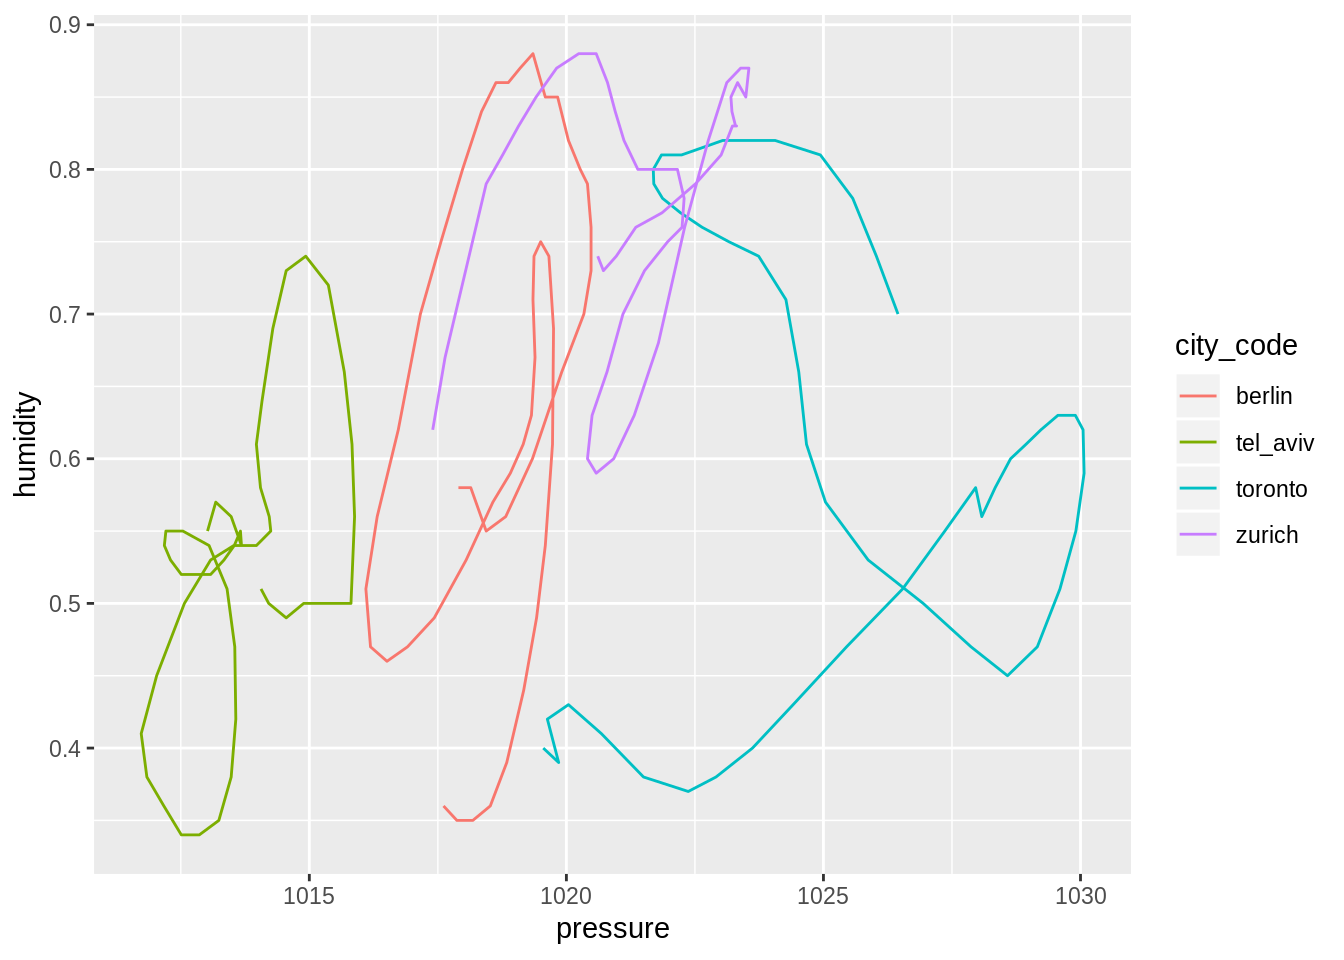
\includegraphics{tidyprog_files/figure-latex/12-visibility-vs-humitidy-1.pdf}

Barplots of number of occurences of each kind of weather per city:

\begin{Shaded}
\begin{Highlighting}[]
\NormalTok{weather_data }\OperatorTok
\StringTok{  }\KeywordTok{ggplot}\NormalTok{(}\KeywordTok{aes}\NormalTok{(}\DataTypeTok{x =}\NormalTok{ city_code)) }\OperatorTok{+}
\StringTok{  }\KeywordTok{geom_bar}\NormalTok{(}\KeywordTok{aes}\NormalTok{(}\DataTypeTok{fill =}\NormalTok{ summary))}
\end{Highlighting}
\end{Shaded}

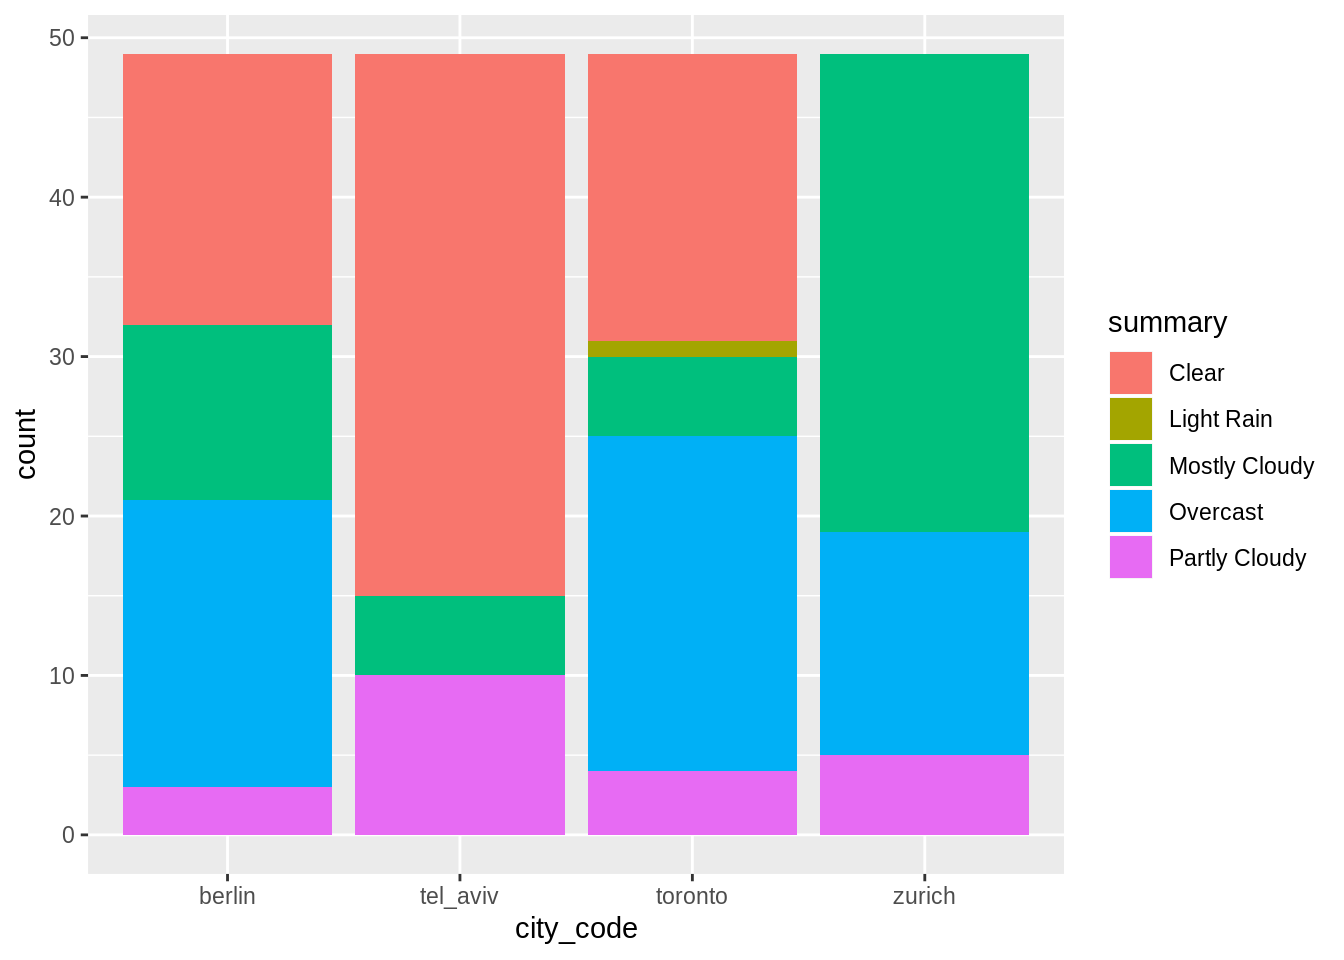
\includegraphics{tidyprog_files/figure-latex/12-summary-1.pdf}

\begin{Shaded}
\begin{Highlighting}[]
\NormalTok{weather_data }\OperatorTok
\StringTok{  }\KeywordTok{ggplot}\NormalTok{(}\KeywordTok{aes}\NormalTok{(}\DataTypeTok{x =}\NormalTok{ city_code)) }\OperatorTok{+}
\StringTok{  }\KeywordTok{geom_bar}\NormalTok{(}\KeywordTok{aes}\NormalTok{(}\DataTypeTok{fill =}\NormalTok{ summary), }\DataTypeTok{position =} \KeywordTok{position_dodge2}\NormalTok{(}\StringTok{"dodge"}\NormalTok{, }\DataTypeTok{preserve =} \StringTok{"single"}\NormalTok{))}
\end{Highlighting}
\end{Shaded}

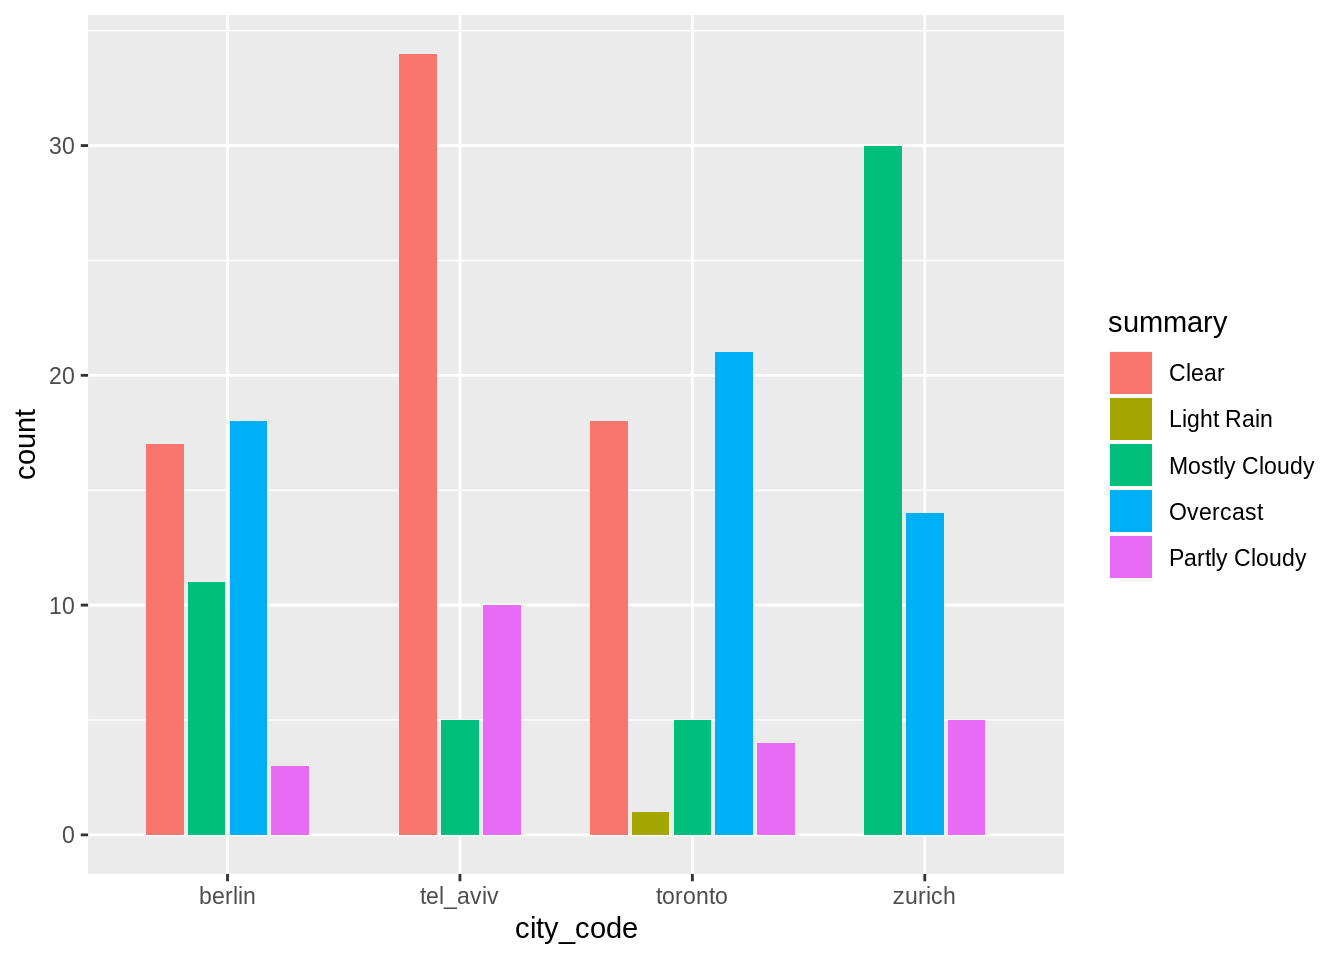
\includegraphics{tidyprog_files/figure-latex/12-summary-2.pdf}

Lineplot with different line types and an additional visualisation of the line range (here, difference between apparent and actual temperature):

\begin{Shaded}
\begin{Highlighting}[]
\NormalTok{weather_data }\OperatorTok
\StringTok{  }\KeywordTok{select}\NormalTok{(city_code, time, temperature, apparentTemperature) }\OperatorTok
\StringTok{  }\KeywordTok{gather}\NormalTok{(kind, temperature, }\OperatorTok{-}\NormalTok{city_code, }\OperatorTok{-}\NormalTok{time)}
\end{Highlighting}
\end{Shaded}

\begin{verbatim}
## # A tibble: 392 x 4
##   city_code time                kind        temperature
##   <chr>     <dttm>              <chr>             <dbl>
## 1 berlin    2019-04-28 15:00:00 temperature        13.4
## 2 berlin    2019-04-28 16:00:00 temperature        13.6
## 3 berlin    2019-04-28 17:00:00 temperature        14.1
## # ... with 389 more rows
\end{verbatim}

\begin{Shaded}
\begin{Highlighting}[]
\NormalTok{temperature_data <-}
\StringTok{  }\NormalTok{weather_data }\OperatorTok
\StringTok{  }\KeywordTok{select}\NormalTok{(city_code, time, temperature, apparentTemperature) }\OperatorTok
\StringTok{  }\KeywordTok{gather}\NormalTok{(kind, temperature, }\OperatorTok{-}\NormalTok{city_code, }\OperatorTok{-}\NormalTok{time) }\OperatorTok
\StringTok{  }\KeywordTok{mutate}\NormalTok{(}\DataTypeTok{apparent =}\NormalTok{ (kind }\OperatorTok{==}\StringTok{ "apparentTemperature"}\NormalTok{)) }\OperatorTok
\StringTok{  }\KeywordTok{select}\NormalTok{(}\OperatorTok{-}\NormalTok{kind)}

\NormalTok{temperature_data}
\end{Highlighting}
\end{Shaded}

\begin{verbatim}
## # A tibble: 392 x 4
##   city_code time                temperature apparent
##   <chr>     <dttm>                    <dbl> <lgl>   
## 1 berlin    2019-04-28 15:00:00        13.4 FALSE   
## 2 berlin    2019-04-28 16:00:00        13.6 FALSE   
## 3 berlin    2019-04-28 17:00:00        14.1 FALSE   
## # ... with 389 more rows
\end{verbatim}

\begin{Shaded}
\begin{Highlighting}[]
\NormalTok{temperature_data }\OperatorTok
\StringTok{  }\KeywordTok{ggplot}\NormalTok{(}\KeywordTok{aes}\NormalTok{(}\DataTypeTok{x =}\NormalTok{ time, }\DataTypeTok{color =}\NormalTok{ city_code)) }\OperatorTok{+}
\StringTok{  }\KeywordTok{geom_linerange}\NormalTok{(}\DataTypeTok{data =}\NormalTok{ weather_data, }\KeywordTok{aes}\NormalTok{(}\DataTypeTok{ymin =}\NormalTok{ temperature, }\DataTypeTok{ymax =}\NormalTok{ apparentTemperature)) }\OperatorTok{+}
\StringTok{  }\KeywordTok{geom_line}\NormalTok{(}\KeywordTok{aes}\NormalTok{(}\DataTypeTok{linetype =}\NormalTok{ apparent, }\DataTypeTok{y =}\NormalTok{ temperature))}
\end{Highlighting}
\end{Shaded}

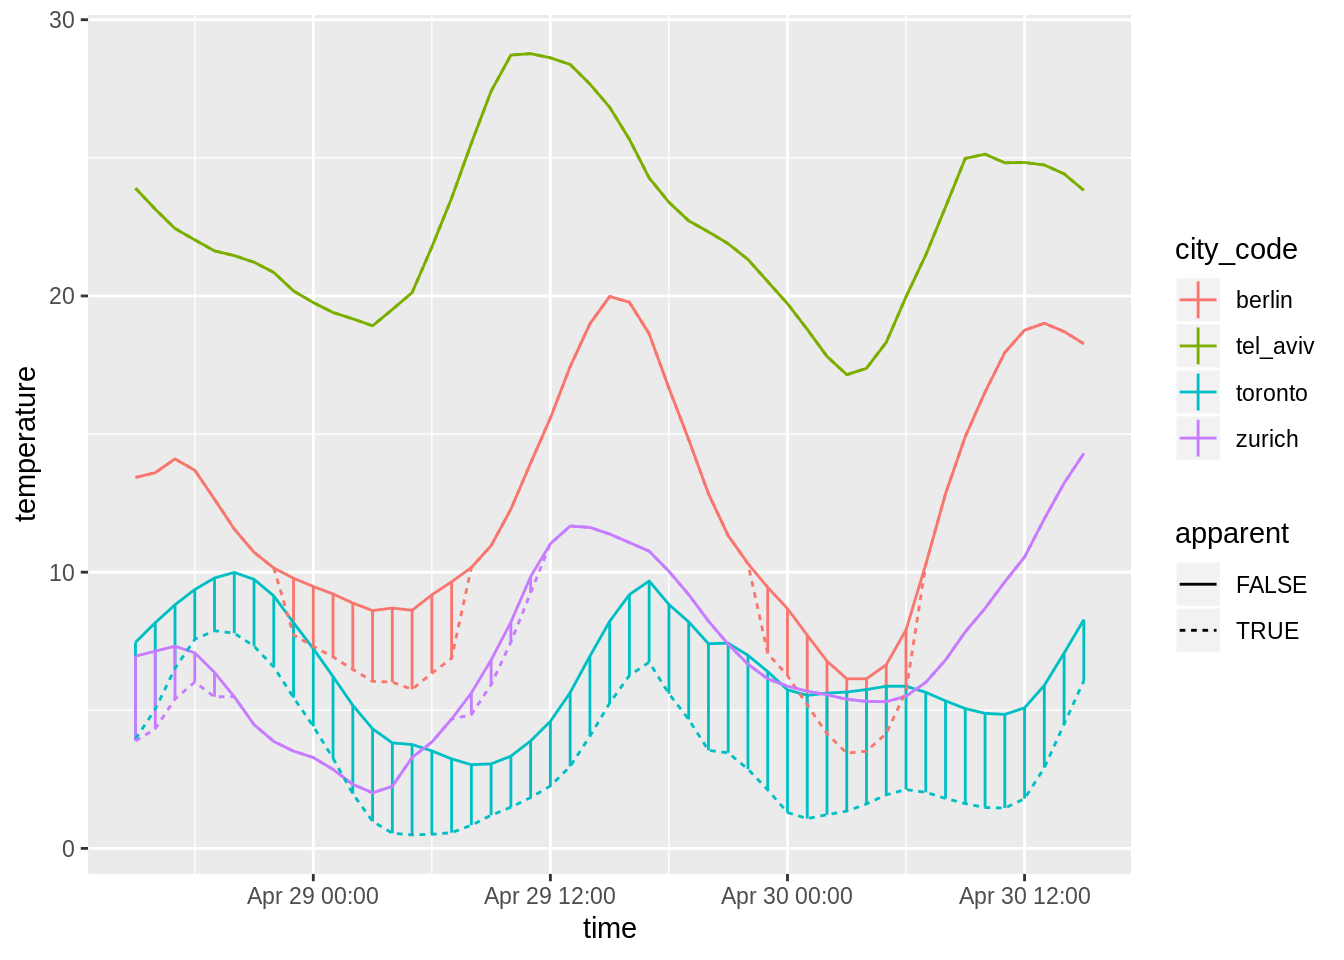
\includegraphics{tidyprog_files/figure-latex/12-temperature-and-apparent-temperature-1.pdf}

Relation of temperature difference between actual and apparent temperature (cf.~line range in last plot) with wind speed, shown as scatter plot.

\begin{Shaded}
\begin{Highlighting}[]
\NormalTok{weather_data }\OperatorTok
\StringTok{  }\KeywordTok{mutate}\NormalTok{(}\DataTypeTok{apparentTemperatureReduction =}\NormalTok{ temperature }\OperatorTok{-}\StringTok{ }\NormalTok{apparentTemperature) }\OperatorTok
\StringTok{  }\KeywordTok{filter}\NormalTok{(city_code }\OperatorTok{!=}\StringTok{ "tel_aviv"}\NormalTok{) }\OperatorTok
\StringTok{  }\KeywordTok{ggplot}\NormalTok{(}\KeywordTok{aes}\NormalTok{(}\DataTypeTok{x =}\NormalTok{ windSpeed, }\DataTypeTok{y =}\NormalTok{ apparentTemperatureReduction)) }\OperatorTok{+}
\StringTok{  }\KeywordTok{geom_point}\NormalTok{(}\KeywordTok{aes}\NormalTok{(}\DataTypeTok{color =}\NormalTok{ city_code))}
\end{Highlighting}
\end{Shaded}

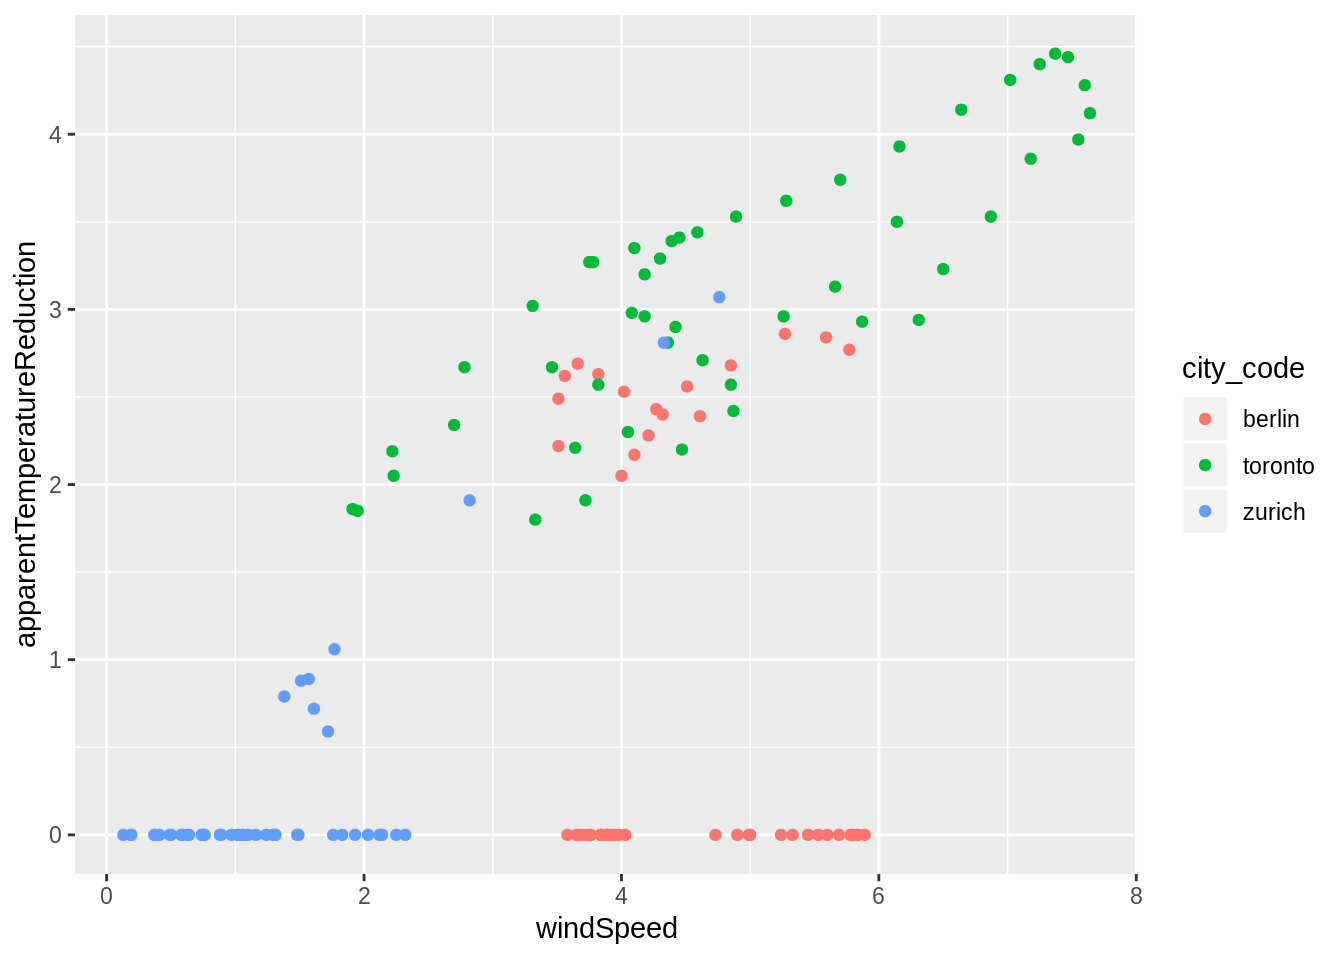
\includegraphics{tidyprog_files/figure-latex/12-compute-and-plot-temperature-difference-1.pdf}

\hypertarget{further-dplyr-transformations}{%
\subsection{Further dplyr transformations}\label{further-dplyr-transformations}}

If you want to compare measurements of the same observable at two different points in time, maybe the most straightforward way to do so is to create a new column with an appropriate lag:

\begin{Shaded}
\begin{Highlighting}[]
\NormalTok{weather_data }\OperatorTok
\StringTok{  }\KeywordTok{group_by}\NormalTok{(city_code) }\OperatorTok
\StringTok{  }\KeywordTok{mutate_at}\NormalTok{(}\KeywordTok{vars}\NormalTok{(temperature, pressure, humidity), }\KeywordTok{list}\NormalTok{(}\DataTypeTok{lag =}\NormalTok{ lag)) }\OperatorTok
\StringTok{  }\KeywordTok{ungroup}\NormalTok{()}
\end{Highlighting}
\end{Shaded}

\begin{verbatim}
## # A tibble: 196 x 22
##   city_code time                summary icon  precipIntensity
##   <chr>     <dttm>              <chr>   <chr>           <dbl>
## 1 berlin    2019-04-28 15:00:00 Mostly~ part~               0
## 2 berlin    2019-04-28 16:00:00 Mostly~ part~               0
## 3 berlin    2019-04-28 17:00:00 Mostly~ part~               0
## # ... with 193 more rows, and 17 more variables: precipProbability <dbl>,
## #   temperature <dbl>, apparentTemperature <dbl>, dewPoint <dbl>,
## #   humidity <dbl>, pressure <dbl>, windSpeed <dbl>, windGust <dbl>,
## #   windBearing <dbl>, cloudCover <dbl>, uvIndex <dbl>, visibility <dbl>,
## #   ozone <dbl>, precipType <chr>, temperature_lag <dbl>,
## #   pressure_lag <dbl>, humidity_lag <dbl>
\end{verbatim}

Count observations per category or combinations of categories:

\begin{Shaded}
\begin{Highlighting}[]
\NormalTok{weather_data }\OperatorTok
\StringTok{  }\KeywordTok{count}\NormalTok{(city_code)}
\end{Highlighting}
\end{Shaded}

\begin{verbatim}
## # A tibble: 4 x 2
##   city_code     n
##   <chr>     <int>
## 1 berlin       49
## 2 tel_aviv     49
## 3 toronto      49
## 4 zurich       49
\end{verbatim}

\begin{Shaded}
\begin{Highlighting}[]
\NormalTok{weather_data }\OperatorTok
\StringTok{  }\KeywordTok{count}\NormalTok{(city_code, summary)}
\end{Highlighting}
\end{Shaded}

\begin{verbatim}
## # A tibble: 15 x 3
##   city_code summary           n
##   <chr>     <chr>         <int>
## 1 berlin    Clear            17
## 2 berlin    Mostly Cloudy    11
## 3 berlin    Overcast         18
## # ... with 12 more rows
\end{verbatim}

Use \texttt{summarize()} to create a tibble with mean and maximum temperature for each city:

\begin{Shaded}
\begin{Highlighting}[]
\NormalTok{weather_data }\OperatorTok
\StringTok{  }\KeywordTok{group_by}\NormalTok{(city_code) }\OperatorTok
\StringTok{  }\KeywordTok{summarize}\NormalTok{(}\DataTypeTok{temperature_mean =} \KeywordTok{mean}\NormalTok{(temperature), }\DataTypeTok{temperature_max =} \KeywordTok{max}\NormalTok{(temperature)) }\OperatorTok
\StringTok{  }\KeywordTok{ungroup}\NormalTok{()}
\end{Highlighting}
\end{Shaded}

\begin{verbatim}
## # A tibble: 4 x 3
##   city_code temperature_mean temperature_max
##   <chr>                <dbl>           <dbl>
## 1 berlin               12.5            20.0 
## 2 tel_aviv             22.6            28.8 
## 3 toronto               6.39            9.99
## 4 zurich                7.15           14.3
\end{verbatim}

Compute and display summary data for all numeric variables:

\begin{Shaded}
\begin{Highlighting}[]
\NormalTok{weather_data }\OperatorTok
\StringTok{  }\KeywordTok{group_by}\NormalTok{(city_code) }\OperatorTok
\StringTok{  }\KeywordTok{summarize_if}\NormalTok{(is.numeric, }\KeywordTok{list}\NormalTok{(}\DataTypeTok{mean =}\NormalTok{ mean, }\DataTypeTok{sd =}\NormalTok{ sd, }\DataTypeTok{min =}\NormalTok{ min, }\DataTypeTok{max =}\NormalTok{ max)) }\OperatorTok
\StringTok{  }\KeywordTok{ungroup}\NormalTok{() }\OperatorTok
\StringTok{  }\KeywordTok{gather}\NormalTok{(key, value, }\OperatorTok{-}\NormalTok{city_code) }\OperatorTok
\StringTok{  }\KeywordTok{separate}\NormalTok{(key, }\DataTypeTok{into =} \KeywordTok{c}\NormalTok{(}\StringTok{"indicator"}\NormalTok{, }\StringTok{"fun"}\NormalTok{)) }\OperatorTok
\StringTok{  }\KeywordTok{xtabs}\NormalTok{(value }\OperatorTok{~}\StringTok{ }\NormalTok{city_code }\OperatorTok{+}\StringTok{ }\NormalTok{indicator }\OperatorTok{+}\StringTok{ }\NormalTok{fun, .) }\OperatorTok
\StringTok{  }\KeywordTok{ftable}\NormalTok{()}
\end{Highlighting}
\end{Shaded}

\begin{verbatim}
##                               fun           max          mean           min            sd
## city_code indicator                                                                      
## berlin    apparentTemperature       19.98000000   11.62836735    3.45000000    5.07360997
##           cloudCover                 1.00000000    0.59734694    0.00000000    0.42339292
##           dewPoint                  10.18000000    5.23632653    1.88000000    2.45837742
##           humidity                   0.88000000    0.63448980    0.35000000    0.15571156
##           ozone                    378.04000000  343.34571429  319.68000000   21.60874350
##           precipIntensity            0.34800000    0.03084286    0.00000000    0.07902264
##           precipProbability          0.54000000    0.06000000    0.00000000    0.13913423
##           pressure                1020.48000000 1018.71714286 1016.10000000    1.19202733
##           temperature               19.98000000   12.49795918    6.14000000    4.10004115
##           uvIndex                    5.00000000    1.24489796    0.00000000    1.61413821
##           visibility                16.09000000   15.77102041   10.01000000    1.13380672
##           windBearing              358.00000000  151.59183673    4.00000000  152.79205891
##           windGust                  11.14000000    7.59591837    3.67000000    2.18713275
##           windSpeed                  5.89000000    4.49326531    3.51000000    0.81341458
## tel_aviv  apparentTemperature       28.77000000   22.64591837   17.15000000    3.15235885
##           cloudCover                 0.81000000    0.19693878    0.00000000    0.24908335
##           dewPoint                  14.43000000   12.18244898    9.51000000    1.29219376
##           humidity                   0.74000000    0.52612245    0.34000000    0.09347050
##           ozone                    339.37000000  318.31836735  307.16000000   10.05895835
##           precipIntensity            0.00000000    0.00000000    0.00000000    0.00000000
##           precipProbability          0.00000000    0.00000000    0.00000000    0.00000000
##           pressure                1015.88000000 1013.66265306 1011.73000000    1.12583076
##           temperature               28.77000000   22.64591837   17.15000000    3.15235885
##           uvIndex                   10.00000000    2.40816327    0.00000000    3.56439784
##           visibility                16.09000000   15.87163265   10.01000000    1.07987528
##           windBearing              355.00000000  188.36734694    0.00000000  123.84965581
##           windGust                   5.53000000    3.47775510    1.66000000    1.19411101
##           windSpeed                  4.90000000    2.49285714    0.57000000    1.04899754
## toronto   apparentTemperature        7.88000000    3.27306122    0.49000000    2.24842464
##           cloudCover                 1.00000000    0.59510204    0.00000000    0.43183293
##           dewPoint                   3.05000000   -1.26653061   -5.17000000    2.69193359
##           humidity                   0.82000000    0.59734694    0.37000000    0.14628419
##           ozone                    401.89000000  362.02632653  327.57000000   23.42483179
##           precipIntensity            0.84070000    0.08387551    0.00000000    0.16627247
##           precipProbability          0.51000000    0.06653061    0.00000000    0.11739447
##           pressure                1030.07000000 1025.14918367 1019.55000000    3.22083053
##           temperature                9.99000000    6.38795918    3.03000000    2.02387621
##           uvIndex                    6.00000000    1.40816327    0.00000000    1.84750245
##           visibility                16.09000000   15.14673469    5.13000000    2.83815256
##           windBearing              357.00000000  140.32653061    2.00000000  129.30831820
##           windGust                  11.51000000    7.51020408    2.66000000    2.33711939
##           windSpeed                  7.64000000    4.87510204    1.91000000    1.62389080
## zurich    apparentTemperature       14.30000000    6.88551020    2.01000000    3.14469133
##           cloudCover                 1.00000000    0.80877551    0.37000000    0.15734295
##           dewPoint                   7.23000000    3.38367347   -0.27000000    1.90397030
##           humidity                   0.88000000    0.77551020    0.59000000    0.08304269
##           ozone                    377.57000000  359.81510204  340.69000000   11.33226737
##           precipIntensity            0.26670000    0.07106939    0.00000000    0.05976032
##           precipProbability          0.29000000    0.13326531    0.00000000    0.07816616
##           pressure                1023.55000000 1021.37612245 1017.40000000    1.62120174
##           temperature               14.30000000    7.14510204    2.01000000    3.07049475
##           uvIndex                    4.00000000    1.10204082    0.00000000    1.44690615
##           visibility                16.09000000   12.90938776    3.89000000    4.47872769
##           windBearing              357.00000000  147.61224490   20.00000000  102.66182679
##           windGust                   4.76000000    1.98428571    1.07000000    0.95327506
##           windSpeed                  4.76000000    1.31244898    0.13000000    0.91823774
\end{verbatim}

\hypertarget{function-basics}{%
\chapter{Function basics}\label{function-basics}}

\begin{quote}
Structuring the code to avoid too much copy-pasting
\end{quote}

This chapter discusses functions as building blocks for more expressive and more powerful data analysis code.

\hypertarget{definition-and-execution}{%
\section{Definition and execution}\label{definition-and-execution}}

The following packages are used for this chapter.

\begin{Shaded}
\begin{Highlighting}[]
\KeywordTok{library}\NormalTok{(tidyverse)}
\KeywordTok{library}\NormalTok{(here)}
\end{Highlighting}
\end{Shaded}

Create functions for tasks that need to be executed repeatedly, or to hide implementation details.

\begin{Shaded}
\begin{Highlighting}[]
\NormalTok{read_weather_data <-}\StringTok{ }\ControlFlowTok{function}\NormalTok{() \{}
  \CommentTok{# Read all files}
\NormalTok{  berlin <-}\StringTok{ }\NormalTok{readxl}\OperatorTok{::}\KeywordTok{read_excel}\NormalTok{(}\KeywordTok{here}\NormalTok{(}\StringTok{"data/weather"}\NormalTok{, }\StringTok{"berlin.xlsx"}\NormalTok{))}
\NormalTok{  toronto <-}\StringTok{ }\NormalTok{readxl}\OperatorTok{::}\KeywordTok{read_excel}\NormalTok{(}\KeywordTok{here}\NormalTok{(}\StringTok{"data/weather"}\NormalTok{, }\StringTok{"toronto.xlsx"}\NormalTok{))}
\NormalTok{  tel_aviv <-}\StringTok{ }\NormalTok{readxl}\OperatorTok{::}\KeywordTok{read_excel}\NormalTok{(}\KeywordTok{here}\NormalTok{(}\StringTok{"data/weather"}\NormalTok{, }\StringTok{"tel_aviv.xlsx"}\NormalTok{))}
\NormalTok{  zurich <-}\StringTok{ }\NormalTok{readxl}\OperatorTok{::}\KeywordTok{read_excel}\NormalTok{(}\KeywordTok{here}\NormalTok{(}\StringTok{"data/weather"}\NormalTok{, }\StringTok{"zurich.xlsx"}\NormalTok{))}

  \CommentTok{# Create ensemble dataset}
\NormalTok{  weather_data <-}\StringTok{ }\KeywordTok{bind_rows}\NormalTok{(}
    \DataTypeTok{berlin =}\NormalTok{ berlin,}
    \DataTypeTok{toronto =}\NormalTok{ toronto,}
    \DataTypeTok{tel_aviv =}\NormalTok{ tel_aviv,}
    \DataTypeTok{zurich =}\NormalTok{ zurich,}
    \DataTypeTok{.id =} \StringTok{"city_code"}
\NormalTok{  )}

  \CommentTok{# Return it}
\NormalTok{  weather_data}
\NormalTok{\}}
\end{Highlighting}
\end{Shaded}

Display the code of any function by writing its name without the subsequent parentheses:

\begin{Shaded}
\begin{Highlighting}[]
\NormalTok{read_weather_data}
\end{Highlighting}
\end{Shaded}

\begin{verbatim}
## function() {
##   # Read all files
##   berlin <- readxl::read_excel(here("data/weather", "berlin.xlsx"))
##   toronto <- readxl::read_excel(here("data/weather", "toronto.xlsx"))
##   tel_aviv <- readxl::read_excel(here("data/weather", "tel_aviv.xlsx"))
##   zurich <- readxl::read_excel(here("data/weather", "zurich.xlsx"))
## 
##   # Create ensemble dataset
##   weather_data <- bind_rows(
##     berlin = berlin,
##     toronto = toronto,
##     tel_aviv = tel_aviv,
##     zurich = zurich,
##     .id = "city_code"
##   )
## 
##   # Return it
##   weather_data
## }
## <environment: 0x3336108>
\end{verbatim}

Call the function by adding the parentheses:

\begin{Shaded}
\begin{Highlighting}[]
\KeywordTok{read_weather_data}\NormalTok{()}
\end{Highlighting}
\end{Shaded}

\begin{verbatim}
## # A tibble: 196 x 19
##   city_code time                summary icon  precipIntensity
##   <chr>     <dttm>              <chr>   <chr>           <dbl>
## 1 berlin    2019-04-28 15:00:00 Mostly~ part~               0
## 2 berlin    2019-04-28 16:00:00 Mostly~ part~               0
## 3 berlin    2019-04-28 17:00:00 Mostly~ part~               0
## # ... with 193 more rows, and 14 more variables: precipProbability <dbl>,
## #   temperature <dbl>, apparentTemperature <dbl>, dewPoint <dbl>,
## #   humidity <dbl>, pressure <dbl>, windSpeed <dbl>, windGust <dbl>,
## #   windBearing <dbl>, cloudCover <dbl>, uvIndex <dbl>, visibility <dbl>,
## #   ozone <dbl>, precipType <chr>
\end{verbatim}

Execution of the function does not create new variables in the global environment.
The only object in the global environment is the function itself:

\begin{Shaded}
\begin{Highlighting}[]
\KeywordTok{ls}\NormalTok{()}
\end{Highlighting}
\end{Shaded}

\begin{verbatim}
## [1] "read_weather_data"
\end{verbatim}

A function can also be used as input for a pipe:

\begin{Shaded}
\begin{Highlighting}[]
\KeywordTok{read_weather_data}\NormalTok{() }\OperatorTok
\StringTok{  }\KeywordTok{count}\NormalTok{(city_code)}
\end{Highlighting}
\end{Shaded}

\begin{verbatim}
## # A tibble: 4 x 2
##   city_code     n
##   <chr>     <int>
## 1 berlin       49
## 2 tel_aviv     49
## 3 toronto      49
## 4 zurich       49
\end{verbatim}

To reuse a function value, assign it to a variable:

\begin{Shaded}
\begin{Highlighting}[]
\NormalTok{weather_data <-}\StringTok{ }\KeywordTok{read_weather_data}\NormalTok{()}
\end{Highlighting}
\end{Shaded}

\hypertarget{exercises}{%
\subsection{Exercises}\label{exercises}}

\begin{enumerate}
\def\labelenumi{\arabic{enumi}.}
\item
  Create a modified version of the function to return only data for Toronto and Tel Aviv. Call it.

\begin{Shaded}
\begin{Highlighting}[]
\NormalTok{read_weather_data_non_europe <-}\StringTok{ }\ControlFlowTok{function}\NormalTok{() \{}
\NormalTok{  _______}
\NormalTok{\}}

\NormalTok{_______}
\end{Highlighting}
\end{Shaded}

\begin{verbatim}
## # A tibble: 98 x 19
##   city_code time                summary icon  precipIntensity
##   <chr>     <dttm>              <chr>   <chr>           <dbl>
## 1 toronto   2019-04-28 15:00:00 Partly~ part~               0
## 2 toronto   2019-04-28 16:00:00 Clear   clea~               0
## 3 toronto   2019-04-28 17:00:00 Clear   clea~               0
## # ... with 95 more rows, and 14 more variables: precipProbability <dbl>,
## #   temperature <dbl>, apparentTemperature <dbl>, dewPoint <dbl>,
## #   humidity <dbl>, pressure <dbl>, windSpeed <dbl>, windGust <dbl>,
## #   windBearing <dbl>, cloudCover <dbl>, uvIndex <dbl>, visibility <dbl>,
## #   ozone <dbl>, precipType <chr>
\end{verbatim}
\item
  Compute number of rows for Europe, count observations to validate:

\begin{Shaded}
\begin{Highlighting}[]
\KeywordTok{nrow}\NormalTok{(_____) }\OperatorTok{-}\StringTok{ }\KeywordTok{nrow}\NormalTok{(_____)}
\end{Highlighting}
\end{Shaded}

\begin{verbatim}
## [1] 98
\end{verbatim}
\end{enumerate}

\hypertarget{args}{%
\section{Arguments}\label{args}}

\emph{Click here to show setup code.}

\begin{Shaded}
\begin{Highlighting}[]
\KeywordTok{library}\NormalTok{(tidyverse)}
\KeywordTok{library}\NormalTok{(here)}
\end{Highlighting}
\end{Shaded}

By adding arguments to your functions, you can turn them into tools for a wide range of applications.
But it is advisable to be conservative here: try to minimise the number of arguments to the necessary ones, so the user has a clear and intuitive interface to deal with.

Functions with arguments:

\begin{Shaded}
\begin{Highlighting}[]
\NormalTok{weather_path <-}\StringTok{ }\ControlFlowTok{function}\NormalTok{(filename) \{}
  \CommentTok{# Returned value}
  \KeywordTok{here}\NormalTok{(}\StringTok{"data/weather"}\NormalTok{, filename)}
\NormalTok{\}}

\KeywordTok{weather_path}\NormalTok{(}\StringTok{"milan.xlsx"}\NormalTok{)}
\end{Highlighting}
\end{Shaded}

\begin{verbatim}
## [1] "/home/travis/build/krlmlr/tidyprog/data/weather/milan.xlsx"
\end{verbatim}

Call functions from within functions:

\begin{Shaded}
\begin{Highlighting}[]
\NormalTok{read_weather_data <-}\StringTok{ }\ControlFlowTok{function}\NormalTok{() \{}
  \CommentTok{# Read all files}
\NormalTok{  berlin <-}\StringTok{ }\NormalTok{readxl}\OperatorTok{::}\KeywordTok{read_excel}\NormalTok{(}\KeywordTok{weather_path}\NormalTok{(}\StringTok{"berlin.xlsx"}\NormalTok{))}
\NormalTok{  toronto <-}\StringTok{ }\NormalTok{readxl}\OperatorTok{::}\KeywordTok{read_excel}\NormalTok{(}\KeywordTok{weather_path}\NormalTok{(}\StringTok{"toronto.xlsx"}\NormalTok{))}
\NormalTok{  tel_aviv <-}\StringTok{ }\NormalTok{readxl}\OperatorTok{::}\KeywordTok{read_excel}\NormalTok{(}\KeywordTok{weather_path}\NormalTok{(}\StringTok{"tel_aviv.xlsx"}\NormalTok{))}
\NormalTok{  zurich <-}\StringTok{ }\NormalTok{readxl}\OperatorTok{::}\KeywordTok{read_excel}\NormalTok{(}\KeywordTok{weather_path}\NormalTok{(}\StringTok{"zurich.xlsx"}\NormalTok{))}

  \CommentTok{# Create ensemble dataset}
\NormalTok{  weather_data <-}\StringTok{ }\KeywordTok{bind_rows}\NormalTok{(}
    \DataTypeTok{berlin =}\NormalTok{ berlin,}
    \DataTypeTok{toronto =}\NormalTok{ toronto,}
    \DataTypeTok{tel_aviv =}\NormalTok{ tel_aviv,}
    \DataTypeTok{zurich =}\NormalTok{ zurich,}
    \DataTypeTok{.id =} \StringTok{"city_code"}
\NormalTok{  )}

  \CommentTok{# Return it}
\NormalTok{  weather_data}
\NormalTok{\}}
\end{Highlighting}
\end{Shaded}

The function still needs to be called for testing it.
It is a good practice to always immediately test a the newly created or updated function by running it:

\begin{Shaded}
\begin{Highlighting}[]
\KeywordTok{read_weather_data}\NormalTok{()}
\end{Highlighting}
\end{Shaded}

\begin{verbatim}
## # A tibble: 196 x 19
##   city_code time                summary icon  precipIntensity
##   <chr>     <dttm>              <chr>   <chr>           <dbl>
## 1 berlin    2019-04-28 15:00:00 Mostly~ part~               0
## 2 berlin    2019-04-28 16:00:00 Mostly~ part~               0
## 3 berlin    2019-04-28 17:00:00 Mostly~ part~               0
## # ... with 193 more rows, and 14 more variables: precipProbability <dbl>,
## #   temperature <dbl>, apparentTemperature <dbl>, dewPoint <dbl>,
## #   humidity <dbl>, pressure <dbl>, windSpeed <dbl>, windGust <dbl>,
## #   windBearing <dbl>, cloudCover <dbl>, uvIndex <dbl>, visibility <dbl>,
## #   ozone <dbl>, precipType <chr>
\end{verbatim}

\hypertarget{exercises-1}{%
\subsection{Exercises}\label{exercises-1}}

\begin{enumerate}
\def\labelenumi{\arabic{enumi}.}
\item
  How does the behavior of \texttt{read\_weather\_data()} change if we update the definition of the \texttt{read\_weather()} function as follows:

\begin{Shaded}
\begin{Highlighting}[]
\NormalTok{weather_path <-}\StringTok{ }\ControlFlowTok{function}\NormalTok{(filename) \{}
  \CommentTok{# Returned value}
  \KeywordTok{here}\NormalTok{(}\StringTok{"data"}\NormalTok{, }\StringTok{"weather"}\NormalTok{, filename)}
\NormalTok{\}}
\end{Highlighting}
\end{Shaded}

  Hint: Define this function with a different name and check its output values, before running \texttt{read\_weather\_data()} again.
\end{enumerate}

\hypertarget{intermediate}{%
\section{Use case: Intermediate variables}\label{intermediate}}

\emph{Click here to show setup code.}

\begin{Shaded}
\begin{Highlighting}[]
\KeywordTok{library}\NormalTok{(tidyverse)}
\KeywordTok{library}\NormalTok{(here)}

\NormalTok{weather_path <-}\StringTok{ }\ControlFlowTok{function}\NormalTok{(filename) \{}
  \CommentTok{# Returned value}
  \KeywordTok{here}\NormalTok{(}\StringTok{"data/weather"}\NormalTok{, filename)}
\NormalTok{\}}
\end{Highlighting}
\end{Shaded}

We start with the function \texttt{weather\_path()} from section \protect\hyperlink{args}{``Arguments''}.

Functions can help to avoid having to use intermediate variables:

\begin{Shaded}
\begin{Highlighting}[]
\NormalTok{read_weather_file <-}\StringTok{ }\ControlFlowTok{function}\NormalTok{(filename) \{}
\NormalTok{  readxl}\OperatorTok{::}\KeywordTok{read_excel}\NormalTok{(}\KeywordTok{weather_path}\NormalTok{(filename))}
\NormalTok{\}}

\NormalTok{read_weather_data <-}\StringTok{ }\ControlFlowTok{function}\NormalTok{() \{}
  \CommentTok{# Create ensemble dataset from files on disk}
\NormalTok{  weather_data <-}\StringTok{ }\KeywordTok{bind_rows}\NormalTok{(}
    \DataTypeTok{berlin =} \KeywordTok{read_weather_file}\NormalTok{(}\StringTok{"berlin.xlsx"}\NormalTok{),}
    \DataTypeTok{toronto =} \KeywordTok{read_weather_file}\NormalTok{(}\StringTok{"toronto.xlsx"}\NormalTok{),}
    \DataTypeTok{tel_aviv =} \KeywordTok{read_weather_file}\NormalTok{(}\StringTok{"tel_aviv.xlsx"}\NormalTok{),}
    \DataTypeTok{zurich =} \KeywordTok{read_weather_file}\NormalTok{(}\StringTok{"zurich.xlsx"}\NormalTok{),}
    \DataTypeTok{.id =} \StringTok{"city_code"}
\NormalTok{  )}

  \CommentTok{# Return it}
\NormalTok{  weather_data}
\NormalTok{\}}

\KeywordTok{read_weather_data}\NormalTok{()}
\end{Highlighting}
\end{Shaded}

\begin{verbatim}
## # A tibble: 196 x 19
##   city_code time                summary icon  precipIntensity
##   <chr>     <dttm>              <chr>   <chr>           <dbl>
## 1 berlin    2019-04-28 15:00:00 Mostly~ part~               0
## 2 berlin    2019-04-28 16:00:00 Mostly~ part~               0
## 3 berlin    2019-04-28 17:00:00 Mostly~ part~               0
## # ... with 193 more rows, and 14 more variables: precipProbability <dbl>,
## #   temperature <dbl>, apparentTemperature <dbl>, dewPoint <dbl>,
## #   humidity <dbl>, pressure <dbl>, windSpeed <dbl>, windGust <dbl>,
## #   windBearing <dbl>, cloudCover <dbl>, uvIndex <dbl>, visibility <dbl>,
## #   ozone <dbl>, precipType <chr>
\end{verbatim}

\hypertarget{exercises-2}{%
\subsection{Exercises}\label{exercises-2}}

\begin{enumerate}
\def\labelenumi{\arabic{enumi}.}
\item
  Implement a helper function \texttt{get\_weather\_file\_for()} that takes a city code as input and returns the file name for the corresponding Excel file. Intended usage: \texttt{get\_weather\_file\_for("berlin")}. Test this function on a few example inputs.

\begin{Shaded}
\begin{Highlighting}[]
\NormalTok{get_weather_file_for <-}\StringTok{ }\NormalTok{_____ \{}
  \KeywordTok{paste0}\NormalTok{(city_code, }\StringTok{".xlsx"}\NormalTok{)}
\NormalTok{\}}
\end{Highlighting}
\end{Shaded}

\begin{Shaded}
\begin{Highlighting}[]
\KeywordTok{get_weather_file_for}\NormalTok{(}\StringTok{"munich"}\NormalTok{)}
\end{Highlighting}
\end{Shaded}

\begin{verbatim}
## [1] "munich.xlsx"
\end{verbatim}

\begin{Shaded}
\begin{Highlighting}[]
\KeywordTok{get_weather_file_for}\NormalTok{(}\StringTok{"san_diego"}\NormalTok{)}
\end{Highlighting}
\end{Shaded}

\begin{verbatim}
## [1] "san_diego.xlsx"
\end{verbatim}
\item
  Implement a helper function \texttt{get\_weather\_data\_for()} that takes a city code as input (as opposed to a file name). Intended usage: \texttt{get\_weather\_data\_for("berlin")}. Update \texttt{read\_weather\_data()} to use \texttt{get\_weather\_data\_for()}.

\begin{Shaded}
\begin{Highlighting}[]
\NormalTok{get_weather_data_for <-}\StringTok{ }\NormalTok{_____ \{}
  \KeywordTok{read_weather_file}\NormalTok{(_____)}
\NormalTok{\}}
\end{Highlighting}
\end{Shaded}

\begin{Shaded}
\begin{Highlighting}[]
\KeywordTok{get_weather_data_for}\NormalTok{(}\StringTok{"toronto"}\NormalTok{)}
\end{Highlighting}
\end{Shaded}

\begin{verbatim}
## # A tibble: 49 x 18
##   time                summary icon  precipIntensity precipProbabili~
##   <dttm>              <chr>   <chr>           <dbl>            <dbl>
## 1 2019-04-28 15:00:00 Partly~ part~               0                0
## 2 2019-04-28 16:00:00 Clear   clea~               0                0
## 3 2019-04-28 17:00:00 Clear   clea~               0                0
## # ... with 46 more rows, and 13 more variables: temperature <dbl>,
## #   apparentTemperature <dbl>, dewPoint <dbl>, humidity <dbl>,
## #   pressure <dbl>, windSpeed <dbl>, windGust <dbl>, windBearing <dbl>,
## #   cloudCover <dbl>, uvIndex <dbl>, visibility <dbl>, ozone <dbl>,
## #   precipType <chr>
\end{verbatim}
\end{enumerate}

\hypertarget{default-values}{%
\section{Default values}\label{default-values}}

\emph{Click here to show setup code.}

\begin{Shaded}
\begin{Highlighting}[]
\KeywordTok{library}\NormalTok{(tidyverse)}
\KeywordTok{library}\NormalTok{(here)}


\NormalTok{weather_path <-}\StringTok{ }\ControlFlowTok{function}\NormalTok{(filename) \{}
  \CommentTok{# Returned value}
  \KeywordTok{here}\NormalTok{(}\StringTok{"data/weather"}\NormalTok{, filename)}
\NormalTok{\}}

\NormalTok{read_weather_file <-}\StringTok{ }\ControlFlowTok{function}\NormalTok{(filename) \{}
\NormalTok{  readxl}\OperatorTok{::}\KeywordTok{read_excel}\NormalTok{(}\KeywordTok{weather_path}\NormalTok{(filename))}
\NormalTok{\}}

\NormalTok{get_weather_file_for <-}\StringTok{ }\ControlFlowTok{function}\NormalTok{(city_code) \{}
  \KeywordTok{paste0}\NormalTok{(city_code, }\StringTok{".xlsx"}\NormalTok{)}
\NormalTok{\}}

\NormalTok{get_weather_data_for <-}\StringTok{ }\ControlFlowTok{function}\NormalTok{(city_code) \{}
  \KeywordTok{read_weather_file}\NormalTok{(}\KeywordTok{get_weather_file_for}\NormalTok{(city_code))}
\NormalTok{\}}
\end{Highlighting}
\end{Shaded}

For user-friendliness it is often good practice to provide default values for parameters

We start with the function\texttt{get\_weather\_data\_for()} from section \protect\hyperlink{intermediate}{``Intermediate variables''}.

Here an example of a boolean argument which when \texttt{TRUE} leads to dropping the data about Zurich.

\begin{Shaded}
\begin{Highlighting}[]
\NormalTok{read_weather_data <-}\StringTok{ }\ControlFlowTok{function}\NormalTok{(}\DataTypeTok{omit_zurich =} \OtherTok{FALSE}\NormalTok{) \{}
  \CommentTok{# Create ensemble dataset from files on disk}
\NormalTok{  weather_data <-}\StringTok{ }\KeywordTok{bind_rows}\NormalTok{(}
    \DataTypeTok{berlin =} \KeywordTok{get_weather_data_for}\NormalTok{(}\StringTok{"berlin"}\NormalTok{),}
    \DataTypeTok{toronto =} \KeywordTok{get_weather_data_for}\NormalTok{(}\StringTok{"toronto"}\NormalTok{),}
    \DataTypeTok{tel_aviv =} \KeywordTok{get_weather_data_for}\NormalTok{(}\StringTok{"tel_aviv"}\NormalTok{),}
    \DataTypeTok{zurich =} \KeywordTok{get_weather_data_for}\NormalTok{(}\StringTok{"zurich"}\NormalTok{),}
    \DataTypeTok{.id =} \StringTok{"city_code"}
\NormalTok{  )}

  \CommentTok{# Return it (filtered)}
\NormalTok{  weather_data }\OperatorTok
\StringTok{    }\KeywordTok{filter}\NormalTok{( }\OperatorTok{!}\NormalTok{(city_code }\OperatorTok{==}\StringTok{ "zurich"} \OperatorTok{&}\StringTok{ }\NormalTok{omit_zurich) )}
\NormalTok{\}}
\end{Highlighting}
\end{Shaded}

Set arguments with default values explicitly with or without using the name or leave them out to use the default value:

\begin{Shaded}
\begin{Highlighting}[]
\KeywordTok{read_weather_data}\NormalTok{(}\OtherTok{TRUE}\NormalTok{)}
\end{Highlighting}
\end{Shaded}

\begin{verbatim}
## # A tibble: 147 x 19
##   city_code time                summary icon  precipIntensity
##   <chr>     <dttm>              <chr>   <chr>           <dbl>
## 1 berlin    2019-04-28 15:00:00 Mostly~ part~               0
## 2 berlin    2019-04-28 16:00:00 Mostly~ part~               0
## 3 berlin    2019-04-28 17:00:00 Mostly~ part~               0
## # ... with 144 more rows, and 14 more variables: precipProbability <dbl>,
## #   temperature <dbl>, apparentTemperature <dbl>, dewPoint <dbl>,
## #   humidity <dbl>, pressure <dbl>, windSpeed <dbl>, windGust <dbl>,
## #   windBearing <dbl>, cloudCover <dbl>, uvIndex <dbl>, visibility <dbl>,
## #   ozone <dbl>, precipType <chr>
\end{verbatim}

\begin{Shaded}
\begin{Highlighting}[]
\KeywordTok{read_weather_data}\NormalTok{(}\DataTypeTok{omit_zurich =} \OtherTok{TRUE}\NormalTok{)}
\end{Highlighting}
\end{Shaded}

\begin{verbatim}
## # A tibble: 147 x 19
##   city_code time                summary icon  precipIntensity
##   <chr>     <dttm>              <chr>   <chr>           <dbl>
## 1 berlin    2019-04-28 15:00:00 Mostly~ part~               0
## 2 berlin    2019-04-28 16:00:00 Mostly~ part~               0
## 3 berlin    2019-04-28 17:00:00 Mostly~ part~               0
## # ... with 144 more rows, and 14 more variables: precipProbability <dbl>,
## #   temperature <dbl>, apparentTemperature <dbl>, dewPoint <dbl>,
## #   humidity <dbl>, pressure <dbl>, windSpeed <dbl>, windGust <dbl>,
## #   windBearing <dbl>, cloudCover <dbl>, uvIndex <dbl>, visibility <dbl>,
## #   ozone <dbl>, precipType <chr>
\end{verbatim}

\begin{Shaded}
\begin{Highlighting}[]
\KeywordTok{read_weather_data}\NormalTok{()}
\end{Highlighting}
\end{Shaded}

\begin{verbatim}
## # A tibble: 196 x 19
##   city_code time                summary icon  precipIntensity
##   <chr>     <dttm>              <chr>   <chr>           <dbl>
## 1 berlin    2019-04-28 15:00:00 Mostly~ part~               0
## 2 berlin    2019-04-28 16:00:00 Mostly~ part~               0
## 3 berlin    2019-04-28 17:00:00 Mostly~ part~               0
## # ... with 193 more rows, and 14 more variables: precipProbability <dbl>,
## #   temperature <dbl>, apparentTemperature <dbl>, dewPoint <dbl>,
## #   humidity <dbl>, pressure <dbl>, windSpeed <dbl>, windGust <dbl>,
## #   windBearing <dbl>, cloudCover <dbl>, uvIndex <dbl>, visibility <dbl>,
## #   ozone <dbl>, precipType <chr>
\end{verbatim}

\hypertarget{exercises-3}{%
\subsection{Exercises}\label{exercises-3}}

\begin{enumerate}
\def\labelenumi{\arabic{enumi}.}
\item
  Update \texttt{get\_weather\_data\_for()} to return Zurich data if called without arguments. Is this a good idea?

\begin{Shaded}
\begin{Highlighting}[]
\NormalTok{get_weather_data_for <-}\StringTok{ }\NormalTok{_____ \{}
\NormalTok{  _____}
\NormalTok{\}}
\end{Highlighting}
\end{Shaded}

\begin{Shaded}
\begin{Highlighting}[]
\KeywordTok{get_weather_data_for}\NormalTok{() }\OperatorTok\StringTok{ }
\StringTok{  }\KeywordTok{select}\NormalTok{(temperature)}
\end{Highlighting}
\end{Shaded}

\begin{verbatim}
## # A tibble: 49 x 1
##   temperature
##         <dbl>
## 1        6.96
## 2        7.14
## 3        7.32
## # ... with 46 more rows
\end{verbatim}

\begin{Shaded}
\begin{Highlighting}[]
\KeywordTok{get_weather_data_for}\NormalTok{(}\StringTok{"tel_aviv"}\NormalTok{) }\OperatorTok\StringTok{ }
\StringTok{  }\KeywordTok{select}\NormalTok{(temperature)}
\end{Highlighting}
\end{Shaded}

\begin{verbatim}
## # A tibble: 49 x 1
##   temperature
##         <dbl>
## 1        23.9
## 2        23.1
## 3        22.4
## # ... with 46 more rows
\end{verbatim}
\end{enumerate}

\hypertarget{multiple-arguments}{%
\section{Multiple arguments}\label{multiple-arguments}}

\emph{Click here to show setup code.}

\begin{Shaded}
\begin{Highlighting}[]
\KeywordTok{library}\NormalTok{(tidyverse)}
\KeywordTok{library}\NormalTok{(here)}


\NormalTok{weather_path <-}\StringTok{ }\ControlFlowTok{function}\NormalTok{(filename) \{}
  \CommentTok{# Returned value}
  \KeywordTok{here}\NormalTok{(}\StringTok{"data/weather"}\NormalTok{, filename)}
\NormalTok{\}}

\NormalTok{read_weather_file <-}\StringTok{ }\ControlFlowTok{function}\NormalTok{(filename) \{}
\NormalTok{  readxl}\OperatorTok{::}\KeywordTok{read_excel}\NormalTok{(}\KeywordTok{weather_path}\NormalTok{(filename))}
\NormalTok{\}}

\NormalTok{get_weather_file_for <-}\StringTok{ }\ControlFlowTok{function}\NormalTok{(city_code) \{}
  \KeywordTok{paste0}\NormalTok{(city_code, }\StringTok{".xlsx"}\NormalTok{)}
\NormalTok{\}}

\NormalTok{get_weather_data_for <-}\StringTok{ }\ControlFlowTok{function}\NormalTok{(city_code) \{}
  \KeywordTok{read_weather_file}\NormalTok{(}\KeywordTok{get_weather_file_for}\NormalTok{(city_code))}
\NormalTok{\}}
\end{Highlighting}
\end{Shaded}

We start once more with the functions \texttt{weather\_path()} from section \protect\hyperlink{args}{``Arguments''} and \texttt{get\_weather\_data\_for()} from section \protect\hyperlink{intermediate}{``Intermediate variables''}.

What are the considerations when using multiple function arguments?
You can add new parameters in a very straightforward manner like this:

\begin{Shaded}
\begin{Highlighting}[]
\NormalTok{read_weather_data <-}\StringTok{ }\ControlFlowTok{function}\NormalTok{(}\DataTypeTok{omit_zurich =} \OtherTok{FALSE}\NormalTok{, }\DataTypeTok{omit_toronto =} \OtherTok{FALSE}\NormalTok{) \{}
  \CommentTok{# Create ensemble dataset from files on disk}
\NormalTok{  weather_data <-}\StringTok{ }\KeywordTok{bind_rows}\NormalTok{(}
    \DataTypeTok{berlin =} \KeywordTok{get_weather_data_for}\NormalTok{(}\StringTok{"berlin"}\NormalTok{),}
    \DataTypeTok{toronto =} \KeywordTok{get_weather_data_for}\NormalTok{(}\StringTok{"toronto"}\NormalTok{),}
    \DataTypeTok{tel_aviv =} \KeywordTok{get_weather_data_for}\NormalTok{(}\StringTok{"tel_aviv"}\NormalTok{),}
    \DataTypeTok{zurich =} \KeywordTok{get_weather_data_for}\NormalTok{(}\StringTok{"zurich"}\NormalTok{),}
    \DataTypeTok{.id =} \StringTok{"city_code"}
\NormalTok{  )}

  \CommentTok{# Return it (filtered)}
\NormalTok{  weather_data }\OperatorTok
\StringTok{    }\KeywordTok{filter}\NormalTok{( }\OperatorTok{!}\NormalTok{(city_code }\OperatorTok{==}\StringTok{ "zurich"} \OperatorTok{&}\StringTok{ }\NormalTok{omit_zurich) ) }\OperatorTok
\StringTok{    }\KeywordTok{filter}\NormalTok{( }\OperatorTok{!}\NormalTok{(city_code }\OperatorTok{==}\StringTok{ "toronto"} \OperatorTok{&}\StringTok{ }\NormalTok{omit_toronto) )}
\NormalTok{\}}
\end{Highlighting}
\end{Shaded}

Prefer passing arguments by name rather than only giving the value, especially if the intent of the value is not clear from just reading it.

\begin{Shaded}
\begin{Highlighting}[]
\CommentTok{# Good:}
\KeywordTok{read_weather_data}\NormalTok{(}\DataTypeTok{omit_zurich =} \OtherTok{TRUE}\NormalTok{)}
\end{Highlighting}
\end{Shaded}

\begin{verbatim}
## # A tibble: 147 x 19
##   city_code time                summary icon  precipIntensity
##   <chr>     <dttm>              <chr>   <chr>           <dbl>
## 1 berlin    2019-04-28 15:00:00 Mostly~ part~               0
## 2 berlin    2019-04-28 16:00:00 Mostly~ part~               0
## 3 berlin    2019-04-28 17:00:00 Mostly~ part~               0
## # ... with 144 more rows, and 14 more variables: precipProbability <dbl>,
## #   temperature <dbl>, apparentTemperature <dbl>, dewPoint <dbl>,
## #   humidity <dbl>, pressure <dbl>, windSpeed <dbl>, windGust <dbl>,
## #   windBearing <dbl>, cloudCover <dbl>, uvIndex <dbl>, visibility <dbl>,
## #   ozone <dbl>, precipType <chr>
\end{verbatim}

\begin{Shaded}
\begin{Highlighting}[]
\KeywordTok{read_weather_data}\NormalTok{(}\DataTypeTok{omit_toronto =} \OtherTok{TRUE}\NormalTok{)}
\end{Highlighting}
\end{Shaded}

\begin{verbatim}
## # A tibble: 147 x 19
##   city_code time                summary icon  precipIntensity
##   <chr>     <dttm>              <chr>   <chr>           <dbl>
## 1 berlin    2019-04-28 15:00:00 Mostly~ part~               0
## 2 berlin    2019-04-28 16:00:00 Mostly~ part~               0
## 3 berlin    2019-04-28 17:00:00 Mostly~ part~               0
## # ... with 144 more rows, and 14 more variables: precipProbability <dbl>,
## #   temperature <dbl>, apparentTemperature <dbl>, dewPoint <dbl>,
## #   humidity <dbl>, pressure <dbl>, windSpeed <dbl>, windGust <dbl>,
## #   windBearing <dbl>, cloudCover <dbl>, uvIndex <dbl>, visibility <dbl>,
## #   ozone <dbl>, precipType <chr>
\end{verbatim}

\begin{Shaded}
\begin{Highlighting}[]
\CommentTok{# Bad:}
\KeywordTok{read_weather_data}\NormalTok{(}\OtherTok{TRUE}\NormalTok{)}
\end{Highlighting}
\end{Shaded}

\begin{verbatim}
## # A tibble: 147 x 19
##   city_code time                summary icon  precipIntensity
##   <chr>     <dttm>              <chr>   <chr>           <dbl>
## 1 berlin    2019-04-28 15:00:00 Mostly~ part~               0
## 2 berlin    2019-04-28 16:00:00 Mostly~ part~               0
## 3 berlin    2019-04-28 17:00:00 Mostly~ part~               0
## # ... with 144 more rows, and 14 more variables: precipProbability <dbl>,
## #   temperature <dbl>, apparentTemperature <dbl>, dewPoint <dbl>,
## #   humidity <dbl>, pressure <dbl>, windSpeed <dbl>, windGust <dbl>,
## #   windBearing <dbl>, cloudCover <dbl>, uvIndex <dbl>, visibility <dbl>,
## #   ozone <dbl>, precipType <chr>
\end{verbatim}

Use the so called ellipsis (\texttt{...}) when you want to provide the possibility for the user to call your function with a list of arguments of unspecified length.
This can be e.g.~useful for passing arguments downstream:

\begin{Shaded}
\begin{Highlighting}[]
\NormalTok{weather_path <-}\StringTok{ }\ControlFlowTok{function}\NormalTok{(...) \{}
  \CommentTok{# All arguments are passed on}
  \KeywordTok{here}\NormalTok{(}\StringTok{"data/weather"}\NormalTok{, ...)}
\NormalTok{\}}

\KeywordTok{weather_path}\NormalTok{(}\StringTok{"berlin.xlsx"}\NormalTok{)}
\end{Highlighting}
\end{Shaded}

\begin{verbatim}
## [1] "/home/travis/build/krlmlr/tidyprog/data/weather/berlin.xlsx"
\end{verbatim}

\begin{Shaded}
\begin{Highlighting}[]
\KeywordTok{weather_path}\NormalTok{(}\StringTok{"some"}\NormalTok{, }\StringTok{"subdir"}\NormalTok{, }\StringTok{"with"}\NormalTok{, }\StringTok{"a"}\NormalTok{, }\StringTok{"file.csv"}\NormalTok{)}
\end{Highlighting}
\end{Shaded}

\begin{verbatim}
## [1] "/home/travis/build/krlmlr/tidyprog/data/weather/some/subdir/with/a/file.csv"
\end{verbatim}

Mind, that despite altering the original function and adding new features to it, the original call still works as before:

\begin{Shaded}
\begin{Highlighting}[]
\KeywordTok{read_weather_data}\NormalTok{()}
\end{Highlighting}
\end{Shaded}

\begin{verbatim}
## # A tibble: 196 x 19
##   city_code time                summary icon  precipIntensity
##   <chr>     <dttm>              <chr>   <chr>           <dbl>
## 1 berlin    2019-04-28 15:00:00 Mostly~ part~               0
## 2 berlin    2019-04-28 16:00:00 Mostly~ part~               0
## 3 berlin    2019-04-28 17:00:00 Mostly~ part~               0
## # ... with 193 more rows, and 14 more variables: precipProbability <dbl>,
## #   temperature <dbl>, apparentTemperature <dbl>, dewPoint <dbl>,
## #   humidity <dbl>, pressure <dbl>, windSpeed <dbl>, windGust <dbl>,
## #   windBearing <dbl>, cloudCover <dbl>, uvIndex <dbl>, visibility <dbl>,
## #   ozone <dbl>, precipType <chr>
\end{verbatim}

\hypertarget{exercises-4}{%
\subsection{Exercises}\label{exercises-4}}

\begin{enumerate}
\def\labelenumi{\arabic{enumi}.}
\item
  What does the following return? Why?

\begin{Shaded}
\begin{Highlighting}[]
\KeywordTok{read_weather_data}\NormalTok{(}\OtherTok{TRUE}\NormalTok{, }\DataTypeTok{omit_z =} \OtherTok{FALSE}\NormalTok{) }\OperatorTok
\StringTok{  }\KeywordTok{count}\NormalTok{(city_code)}
\end{Highlighting}
\end{Shaded}

  See the next section for ideas on avoiding this behavior.
\end{enumerate}

\hypertarget{argument-matching}{%
\section{Argument matching}\label{argument-matching}}

\emph{Click here to show setup code.}

How does \texttt{R} handle function calls with arguments?

Named arguments are assigned first, after that remaining slots are filled from left to right.

\begin{Shaded}
\begin{Highlighting}[]
\NormalTok{use_names <-}\StringTok{ }\ControlFlowTok{function}\NormalTok{(}\DataTypeTok{one =} \DecValTok{1}\NormalTok{, }\DataTypeTok{two =} \DecValTok{2}\NormalTok{) \{}
  \KeywordTok{list}\NormalTok{(}\DataTypeTok{one =}\NormalTok{ one, }\DataTypeTok{two =}\NormalTok{ two)}
\NormalTok{\}}

\KeywordTok{use_names}\NormalTok{(}\DecValTok{3}\NormalTok{, }\DecValTok{4}\NormalTok{)}
\end{Highlighting}
\end{Shaded}

\begin{verbatim}
## $one
## [1] 3
## 
## $two
## [1] 4
\end{verbatim}

\begin{Shaded}
\begin{Highlighting}[]
\KeywordTok{use_names}\NormalTok{(}\DataTypeTok{one =} \DecValTok{3}\NormalTok{, }\DecValTok{4}\NormalTok{)}
\end{Highlighting}
\end{Shaded}

\begin{verbatim}
## $one
## [1] 3
## 
## $two
## [1] 4
\end{verbatim}

\begin{Shaded}
\begin{Highlighting}[]
\KeywordTok{use_names}\NormalTok{(}\DecValTok{3}\NormalTok{, }\DataTypeTok{one =} \DecValTok{4}\NormalTok{)}
\end{Highlighting}
\end{Shaded}

\begin{verbatim}
## $one
## [1] 4
## 
## $two
## [1] 3
\end{verbatim}

\begin{Shaded}
\begin{Highlighting}[]
\KeywordTok{use_names}\NormalTok{(}\DataTypeTok{one =} \DecValTok{3}\NormalTok{, }\DataTypeTok{two =} \DecValTok{4}\NormalTok{)}
\end{Highlighting}
\end{Shaded}

\begin{verbatim}
## $one
## [1] 3
## 
## $two
## [1] 4
\end{verbatim}

\begin{Shaded}
\begin{Highlighting}[]
\KeywordTok{use_names}\NormalTok{(}\DataTypeTok{two =} \DecValTok{3}\NormalTok{, }\DataTypeTok{one =} \DecValTok{4}\NormalTok{)}
\end{Highlighting}
\end{Shaded}

\begin{verbatim}
## $one
## [1] 4
## 
## $two
## [1] 3
\end{verbatim}

Arguments are matched partially, which can be convenient but is also a source of errors.

\begin{Shaded}
\begin{Highlighting}[]
\KeywordTok{use_names}\NormalTok{(}\DataTypeTok{o =} \DecValTok{3}\NormalTok{, }\DecValTok{4}\NormalTok{)}
\end{Highlighting}
\end{Shaded}

\begin{verbatim}
## $one
## [1] 3
## 
## $two
## [1] 4
\end{verbatim}

\begin{Shaded}
\begin{Highlighting}[]
\KeywordTok{use_names}\NormalTok{(}\DecValTok{3}\NormalTok{, }\DataTypeTok{o =} \DecValTok{4}\NormalTok{)}
\end{Highlighting}
\end{Shaded}

\begin{verbatim}
## $one
## [1] 4
## 
## $two
## [1] 3
\end{verbatim}

\begin{Shaded}
\begin{Highlighting}[]
\KeywordTok{use_names}\NormalTok{(}\DataTypeTok{o =} \DecValTok{3}\NormalTok{, }\DataTypeTok{t =} \DecValTok{4}\NormalTok{)}
\end{Highlighting}
\end{Shaded}

\begin{verbatim}
## $one
## [1] 3
## 
## $two
## [1] 4
\end{verbatim}

\begin{Shaded}
\begin{Highlighting}[]
\KeywordTok{use_names}\NormalTok{(}\DataTypeTok{t =} \DecValTok{3}\NormalTok{, }\DataTypeTok{o =} \DecValTok{4}\NormalTok{)}
\end{Highlighting}
\end{Shaded}

\begin{verbatim}
## $one
## [1] 4
## 
## $two
## [1] 3
\end{verbatim}

The ellipsis can be used to enforce the user to fully name the function parameters when setting them:

\begin{Shaded}
\begin{Highlighting}[]
\NormalTok{only_names <-}\StringTok{ }\ControlFlowTok{function}\NormalTok{(..., }\DataTypeTok{one =} \DecValTok{1}\NormalTok{, }\DataTypeTok{two =} \DecValTok{2}\NormalTok{) \{}
  \KeywordTok{list}\NormalTok{(}\DataTypeTok{one =}\NormalTok{ one, }\DataTypeTok{two =}\NormalTok{ two)}
\NormalTok{\}}

\KeywordTok{only_names}\NormalTok{(}\DecValTok{3}\NormalTok{, }\DecValTok{4}\NormalTok{)}
\end{Highlighting}
\end{Shaded}

\begin{verbatim}
## $one
## [1] 1
## 
## $two
## [1] 2
\end{verbatim}

\begin{Shaded}
\begin{Highlighting}[]
\KeywordTok{only_names}\NormalTok{(}\DataTypeTok{one =} \DecValTok{3}\NormalTok{, }\DecValTok{4}\NormalTok{)}
\end{Highlighting}
\end{Shaded}

\begin{verbatim}
## $one
## [1] 3
## 
## $two
## [1] 2
\end{verbatim}

\begin{Shaded}
\begin{Highlighting}[]
\KeywordTok{only_names}\NormalTok{(}\DataTypeTok{one =} \DecValTok{3}\NormalTok{, }\DataTypeTok{two =} \DecValTok{4}\NormalTok{)}
\end{Highlighting}
\end{Shaded}

\begin{verbatim}
## $one
## [1] 3
## 
## $two
## [1] 4
\end{verbatim}

\begin{Shaded}
\begin{Highlighting}[]
\KeywordTok{only_names}\NormalTok{(}\DataTypeTok{o =} \DecValTok{3}\NormalTok{, }\DataTypeTok{t =} \DecValTok{4}\NormalTok{)}
\end{Highlighting}
\end{Shaded}

\begin{verbatim}
## $one
## [1] 1
## 
## $two
## [1] 2
\end{verbatim}

Inside a function with an ellipsis as a parameter, you can capture the ellipsis with \texttt{list()}:

\begin{Shaded}
\begin{Highlighting}[]
\NormalTok{ellipsis_test <-}\StringTok{ }\ControlFlowTok{function}\NormalTok{(...) \{}
\NormalTok{  args <-}\StringTok{ }\KeywordTok{list}\NormalTok{(...)}
  \KeywordTok{names}\NormalTok{(args)}
\NormalTok{\}}

\KeywordTok{ellipsis_test}\NormalTok{(}\DataTypeTok{a =} \DecValTok{1}\NormalTok{, }\DecValTok{2}\NormalTok{, }\DataTypeTok{c =} \DecValTok{3}\OperatorTok{:}\DecValTok{5}\NormalTok{)}
\end{Highlighting}
\end{Shaded}

\begin{verbatim}
## [1] "a" ""  "c"
\end{verbatim}

Arguments in ellipsis can be accessed with \texttt{..1}, \texttt{..2} etc.

\begin{Shaded}
\begin{Highlighting}[]
\NormalTok{ellipsis_direct_test <-}\StringTok{ }\ControlFlowTok{function}\NormalTok{(...) \{}
  \KeywordTok{list}\NormalTok{(..}\DecValTok{1}\NormalTok{, ..}\DecValTok{2}\NormalTok{)}
\NormalTok{\}}

\KeywordTok{ellipsis_direct_test}\NormalTok{(}\DataTypeTok{a =} \DecValTok{1}\NormalTok{, }\DecValTok{2}\NormalTok{, }\DataTypeTok{c =} \DecValTok{3}\OperatorTok{:}\DecValTok{5}\NormalTok{)}
\end{Highlighting}
\end{Shaded}

\begin{verbatim}
## [[1]]
## [1] 1
## 
## [[2]]
## [1] 2
\end{verbatim}

\hypertarget{exercises-5}{%
\subsection{Exercises}\label{exercises-5}}

\begin{enumerate}
\def\labelenumi{\arabic{enumi}.}
\item
  Naming, not naming or partly naming parameters in functions calls? What does the following return and why?

\begin{Shaded}
\begin{Highlighting}[]
\NormalTok{use_some_names <-}\StringTok{ }\ControlFlowTok{function}\NormalTok{(}\DataTypeTok{one =} \DecValTok{1}\NormalTok{, ..., }\DataTypeTok{two =} \DecValTok{2}\NormalTok{) \{}
  \KeywordTok{list}\NormalTok{(}\DataTypeTok{one =}\NormalTok{ one, }\DataTypeTok{two =}\NormalTok{ two)}
\NormalTok{\}}

\KeywordTok{use_some_names}\NormalTok{(}\DecValTok{3}\NormalTok{, }\DecValTok{4}\NormalTok{)}
\KeywordTok{use_some_names}\NormalTok{(}\DataTypeTok{one =} \DecValTok{3}\NormalTok{, }\DecValTok{4}\NormalTok{)}
\KeywordTok{use_some_names}\NormalTok{(}\DecValTok{3}\NormalTok{, }\DataTypeTok{one =} \DecValTok{4}\NormalTok{)}
\KeywordTok{use_some_names}\NormalTok{(}\DataTypeTok{one =} \DecValTok{3}\NormalTok{, }\DataTypeTok{two =} \DecValTok{4}\NormalTok{)}
\KeywordTok{use_some_names}\NormalTok{(}\DataTypeTok{two =} \DecValTok{4}\NormalTok{, }\DecValTok{3}\NormalTok{)}
\end{Highlighting}
\end{Shaded}
\item
  Model a new \texttt{enforce\_names()} function after \texttt{only\_names()} to check if any unnamed or misnamed arguments have been used. Test this function in various combinations.

\begin{Shaded}
\begin{Highlighting}[]
\NormalTok{enforce_names <-}\StringTok{ }\ControlFlowTok{function}\NormalTok{(..., }\DataTypeTok{one =} \DecValTok{1}\NormalTok{, }\DataTypeTok{two =} \DecValTok{2}\NormalTok{) \{}
\NormalTok{  extra_args <-}\StringTok{ }\NormalTok{_____}
  \KeywordTok{stopifnot}\NormalTok{(}\KeywordTok{length}\NormalTok{(_____) }\OperatorTok{==}\StringTok{ }\DecValTok{0}\NormalTok{)}

  \KeywordTok{list}\NormalTok{(_____)}
\NormalTok{\}}
\end{Highlighting}
\end{Shaded}

\begin{Shaded}
\begin{Highlighting}[]
\KeywordTok{try}\NormalTok{(}\KeywordTok{enforce_names}\NormalTok{(}\DecValTok{3}\NormalTok{, }\DecValTok{4}\NormalTok{))}
\end{Highlighting}
\end{Shaded}

\begin{verbatim}
## Error in enforce_names(3, 4) : length(extra_args) == 0 is not TRUE
\end{verbatim}

\begin{Shaded}
\begin{Highlighting}[]
\KeywordTok{try}\NormalTok{(}\KeywordTok{enforce_names}\NormalTok{(}\DataTypeTok{one =} \DecValTok{3}\NormalTok{, }\DecValTok{4}\NormalTok{))}
\end{Highlighting}
\end{Shaded}

\begin{verbatim}
## Error in enforce_names(one = 3, 4) : length(extra_args) == 0 is not TRUE
\end{verbatim}

\begin{Shaded}
\begin{Highlighting}[]
\KeywordTok{try}\NormalTok{(}\KeywordTok{enforce_names}\NormalTok{(}\DecValTok{3}\NormalTok{, }\DataTypeTok{one =} \DecValTok{4}\NormalTok{))}
\end{Highlighting}
\end{Shaded}

\begin{verbatim}
## Error in enforce_names(3, one = 4) : length(extra_args) == 0 is not TRUE
\end{verbatim}

\begin{Shaded}
\begin{Highlighting}[]
\KeywordTok{try}\NormalTok{(}\KeywordTok{enforce_names}\NormalTok{(}\DataTypeTok{two =} \DecValTok{4}\NormalTok{, }\DecValTok{3}\NormalTok{))}
\end{Highlighting}
\end{Shaded}

\begin{verbatim}
## Error in enforce_names(two = 4, 3) : length(extra_args) == 0 is not TRUE
\end{verbatim}

\begin{Shaded}
\begin{Highlighting}[]
\KeywordTok{try}\NormalTok{(}\KeywordTok{enforce_names}\NormalTok{(}\DataTypeTok{o =} \DecValTok{3}\NormalTok{, }\DataTypeTok{t =} \DecValTok{4}\NormalTok{))}
\end{Highlighting}
\end{Shaded}

\begin{verbatim}
## Error in enforce_names(o = 3, t = 4) : 
##   length(extra_args) == 0 is not TRUE
\end{verbatim}

\begin{Shaded}
\begin{Highlighting}[]
\KeywordTok{enforce_names}\NormalTok{(}\DataTypeTok{one =} \DecValTok{3}\NormalTok{, }\DataTypeTok{two =} \DecValTok{4}\NormalTok{)}
\end{Highlighting}
\end{Shaded}

\begin{verbatim}
## $one
## [1] 3
## 
## $two
## [1] 4
\end{verbatim}
\end{enumerate}

\hypertarget{simple-iteration}{%
\chapter{Simple iteration}\label{simple-iteration}}

\begin{quote}
Processing multiple files that contain different parts of the same dataset
\end{quote}

This chapter introduces iteration as a concept to repeat the same operation over a sequence of inputs.
It is largely independent of the previous chapter.

The following packages are required throughout this chapter:

\begin{Shaded}
\begin{Highlighting}[]
\KeywordTok{library}\NormalTok{(tidyverse)}
\KeywordTok{library}\NormalTok{(here)}
\end{Highlighting}
\end{Shaded}

\hypertarget{vectors-and-columns}{%
\section{Vectors and columns}\label{vectors-and-columns}}

So far we focus on the data frame, or tibble, as primary object for data analysis.
Internally, a tibble is a list of vectors of the same length.
Accessing a row in a tibble requires finding the same index in that list of vectors.

Here we explore the relationship between columns of data frames and their corresponding vectors, i.e.~the answer to ``how to get from one to the other?'':

We can e.g.~get a vector with the files in a specific directory of our current project\footnote{function \texttt{here::here()} is taking care of making sure we start from the root directory of our current project} like this:

\begin{Shaded}
\begin{Highlighting}[]
\NormalTok{files <-}\StringTok{ }\KeywordTok{dir}\NormalTok{(}\KeywordTok{here}\NormalTok{(}\StringTok{"data/weather"}\NormalTok{), }\DataTypeTok{full.names =} \OtherTok{TRUE}\NormalTok{)}
\NormalTok{files}
\end{Highlighting}
\end{Shaded}

\begin{verbatim}
## [1] "/home/travis/build/krlmlr/tidyprog/data/weather/berlin.xlsx"  
## [2] "/home/travis/build/krlmlr/tidyprog/data/weather/tel_aviv.xlsx"
## [3] "/home/travis/build/krlmlr/tidyprog/data/weather/toronto.xlsx" 
## [4] "/home/travis/build/krlmlr/tidyprog/data/weather/zurich.xlsx"
\end{verbatim}

You can create a tibble from it using \texttt{tibble::enframe()}:

\begin{Shaded}
\begin{Highlighting}[]
\NormalTok{files_df <-}
\StringTok{  }\NormalTok{files }\OperatorTok
\StringTok{  }\KeywordTok{enframe}\NormalTok{()}

\NormalTok{files_df}
\end{Highlighting}
\end{Shaded}

\begin{verbatim}
## # A tibble: 4 x 2
##    name value                                                        
##   <int> <chr>                                                        
## 1     1 /home/travis/build/krlmlr/tidyprog/data/weather/berlin.xlsx  
## 2     2 /home/travis/build/krlmlr/tidyprog/data/weather/tel_aviv.xlsx
## 3     3 /home/travis/build/krlmlr/tidyprog/data/weather/toronto.xlsx 
## 4     4 /home/travis/build/krlmlr/tidyprog/data/weather/zurich.xlsx
\end{verbatim}

The \texttt{name} column might be unwanted in some cases. Suppress its creation by setting \texttt{name\ =\ NULL}:

\begin{Shaded}
\begin{Highlighting}[]
\NormalTok{files_df_}\DecValTok{1}\NormalTok{ <-}
\StringTok{  }\NormalTok{files }\OperatorTok
\StringTok{  }\KeywordTok{enframe}\NormalTok{(}\DataTypeTok{name =} \OtherTok{NULL}\NormalTok{)}

\NormalTok{files_df_}\DecValTok{1}
\end{Highlighting}
\end{Shaded}

\begin{verbatim}
## # A tibble: 4 x 1
##   value                                                        
##   <chr>                                                        
## 1 /home/travis/build/krlmlr/tidyprog/data/weather/berlin.xlsx  
## 2 /home/travis/build/krlmlr/tidyprog/data/weather/tel_aviv.xlsx
## 3 /home/travis/build/krlmlr/tidyprog/data/weather/toronto.xlsx 
## 4 /home/travis/build/krlmlr/tidyprog/data/weather/zurich.xlsx
\end{verbatim}

Another way to create a tibble from a vector is using \texttt{tibble::tibble()}.
You can name the newly created columns by assigning the vectors they are created from to (quoted or unquoted) column names:

\begin{Shaded}
\begin{Highlighting}[]
\KeywordTok{tibble}\NormalTok{(}\DataTypeTok{filename =}\NormalTok{ files)}
\end{Highlighting}
\end{Shaded}

\begin{verbatim}
## # A tibble: 4 x 1
##   filename                                                     
##   <chr>                                                        
## 1 /home/travis/build/krlmlr/tidyprog/data/weather/berlin.xlsx  
## 2 /home/travis/build/krlmlr/tidyprog/data/weather/tel_aviv.xlsx
## 3 /home/travis/build/krlmlr/tidyprog/data/weather/toronto.xlsx 
## 4 /home/travis/build/krlmlr/tidyprog/data/weather/zurich.xlsx
\end{verbatim}

The other direction -- producing a vector from a tibble column -- works with \texttt{dplyr::pull()}.
By default \texttt{pull()} will turn the rightmost column into a vector and ignore the rest of the tibble:

\begin{Shaded}
\begin{Highlighting}[]
\NormalTok{files_df }\OperatorTok
\StringTok{  }\KeywordTok{pull}\NormalTok{()}
\end{Highlighting}
\end{Shaded}

\begin{verbatim}
## [1] "/home/travis/build/krlmlr/tidyprog/data/weather/berlin.xlsx"  
## [2] "/home/travis/build/krlmlr/tidyprog/data/weather/tel_aviv.xlsx"
## [3] "/home/travis/build/krlmlr/tidyprog/data/weather/toronto.xlsx" 
## [4] "/home/travis/build/krlmlr/tidyprog/data/weather/zurich.xlsx"
\end{verbatim}

Turn a specific column into a vector by providing the desired column name to \texttt{pull()}, either quoted or unquoted:

\begin{Shaded}
\begin{Highlighting}[]
\NormalTok{files_df }\OperatorTok
\StringTok{  }\KeywordTok{pull}\NormalTok{(name)}
\end{Highlighting}
\end{Shaded}

\begin{verbatim}
## [1] 1 2 3 4
\end{verbatim}

\hypertarget{exercises-6}{%
\subsection{Exercises}\label{exercises-6}}

\begin{enumerate}
\def\labelenumi{\arabic{enumi}.}
\item
  Investigate the output of \texttt{fs::dir\_ls()} with \texttt{enframe()}. Explain.

\begin{Shaded}
\begin{Highlighting}[]
\CommentTok{# install.packages("fs")}
\NormalTok{fs}\OperatorTok{::}\KeywordTok{dir_ls}\NormalTok{()}
\NormalTok{fs}\OperatorTok{::}\KeywordTok{dir_ls}\NormalTok{() }\OperatorTok
\StringTok{  }\KeywordTok{___}\NormalTok{()}
\end{Highlighting}
\end{Shaded}

\begin{verbatim}
## # A tibble: 45 x 2
##   name         value       
##   <chr>        <fs::path>  
## 1 1.Rmd        1.Rmd       
## 2 12-intro.Rmd 12-intro.Rmd
## 3 2.Rmd        2.Rmd       
## # ... with 42 more rows
\end{verbatim}
\end{enumerate}

\hypertarget{names}{%
\section{Named vectors and two-column tibbles}\label{names}}

\emph{Click here to show setup code.}

\begin{Shaded}
\begin{Highlighting}[]
\KeywordTok{library}\NormalTok{(tidyverse)}
\KeywordTok{library}\NormalTok{(here)}
\end{Highlighting}
\end{Shaded}

Here we look at tidyverse-functions to work with named vectors and tibbles with more columns and the relations netween the two.

As seen in section \protect\hyperlink{intro-data}{``Data''}, load a table -- here a dictionary detailing information related to an id-like name -- from an MS Excel file with \texttt{readxl::read\_excel()}:

\begin{Shaded}
\begin{Highlighting}[]
\NormalTok{dict <-}\StringTok{ }\NormalTok{readxl}\OperatorTok{::}\KeywordTok{read_excel}\NormalTok{(}\KeywordTok{here}\NormalTok{(}\StringTok{"data/cities.xlsx"}\NormalTok{))}
\NormalTok{dict}
\end{Highlighting}
\end{Shaded}

\begin{verbatim}
## # A tibble: 4 x 5
##   city_code weather_filename           name        lng   lat
##   <chr>     <chr>                      <chr>     <dbl> <dbl>
## 1 berlin    data/weather/berlin.xlsx   Berlin    13.4   52.5
## 2 toronto   data/weather/toronto.xlsx  Toronto  -79.4   43.7
## 3 tel_aviv  data/weather/tel_aviv.xlsx Tel Aviv  34.8   32.1
## 4 zurich    data/weather/zurich.xlsx   Zürich     8.54  47.4
\end{verbatim}

Use \texttt{pull()} as seen in the last chapter:

\begin{Shaded}
\begin{Highlighting}[]
\NormalTok{dict }\OperatorTok
\StringTok{  }\KeywordTok{pull}\NormalTok{(weather_filename)}
\end{Highlighting}
\end{Shaded}

\begin{verbatim}
## [1] "data/weather/berlin.xlsx"   "data/weather/toronto.xlsx" 
## [3] "data/weather/tel_aviv.xlsx" "data/weather/zurich.xlsx"
\end{verbatim}

Create absolute paths using \texttt{here::here()}:

\begin{Shaded}
\begin{Highlighting}[]
\NormalTok{dict }\OperatorTok
\StringTok{  }\KeywordTok{pull}\NormalTok{(weather_filename) }\OperatorTok
\StringTok{  }\KeywordTok{here}\NormalTok{()}
\end{Highlighting}
\end{Shaded}

\begin{verbatim}
## [1] "/home/travis/build/krlmlr/tidyprog/data/weather/berlin.xlsx"  
## [2] "/home/travis/build/krlmlr/tidyprog/data/weather/toronto.xlsx" 
## [3] "/home/travis/build/krlmlr/tidyprog/data/weather/tel_aviv.xlsx"
## [4] "/home/travis/build/krlmlr/tidyprog/data/weather/zurich.xlsx"
\end{verbatim}

Produce a named vector with \texttt{tibble::deframe()}, which is thought as the inverse function to \texttt{enframe()}.
When given a 2-column tibble, \texttt{deframe()} will by default use the first column for the names and the second column for the values of the resulting vector.
When given a 1-column tibble, it creates an unnamed vector.
When given a more-than-2-column tibble, it will use the first two columns as name- and value-columns for the resulting vector, ignore the rest and in addition give a warning that it expects a one- or two-column data frame.

\begin{Shaded}
\begin{Highlighting}[]
\NormalTok{weather_filenames <-}
\StringTok{  }\NormalTok{dict }\OperatorTok
\StringTok{  }\KeywordTok{select}\NormalTok{(city_code, weather_filename) }\OperatorTok
\StringTok{  }\KeywordTok{deframe}\NormalTok{()}
\NormalTok{weather_filenames}
\end{Highlighting}
\end{Shaded}

\begin{verbatim}
##                       berlin                      toronto 
##   "data/weather/berlin.xlsx"  "data/weather/toronto.xlsx" 
##                     tel_aviv                       zurich 
## "data/weather/tel_aviv.xlsx"   "data/weather/zurich.xlsx"
\end{verbatim}

The \texttt{names()} function accesses the names of a vector:

\begin{Shaded}
\begin{Highlighting}[]
\NormalTok{weather_filenames }\OperatorTok
\StringTok{  }\KeywordTok{names}\NormalTok{()}
\end{Highlighting}
\end{Shaded}

\begin{verbatim}
## [1] "berlin"   "toronto"  "tel_aviv" "zurich"
\end{verbatim}

Some operations producing vectors from vectors cause the names to be lost:

\begin{Shaded}
\begin{Highlighting}[]
\KeywordTok{paste0}\NormalTok{(}\StringTok{"'"}\NormalTok{, weather_filenames, }\StringTok{"'"}\NormalTok{)}
\end{Highlighting}
\end{Shaded}

\begin{verbatim}
## [1] "'data/weather/berlin.xlsx'"   "'data/weather/toronto.xlsx'" 
## [3] "'data/weather/tel_aviv.xlsx'" "'data/weather/zurich.xlsx'"
\end{verbatim}

\begin{Shaded}
\begin{Highlighting}[]
\NormalTok{weather_filenames }\OperatorTok
\StringTok{  }\KeywordTok{here}\NormalTok{()}
\end{Highlighting}
\end{Shaded}

\begin{verbatim}
## [1] "/home/travis/build/krlmlr/tidyprog/data/weather/berlin.xlsx"  
## [2] "/home/travis/build/krlmlr/tidyprog/data/weather/toronto.xlsx" 
## [3] "/home/travis/build/krlmlr/tidyprog/data/weather/tel_aviv.xlsx"
## [4] "/home/travis/build/krlmlr/tidyprog/data/weather/zurich.xlsx"
\end{verbatim}

A possible solution can be in many cases to change the order of the transformations, so that the creation of the named vector comes last (or at least later):

\begin{Shaded}
\begin{Highlighting}[]
\NormalTok{dict }\OperatorTok
\StringTok{  }\KeywordTok{mutate}\NormalTok{(}\DataTypeTok{weather_filename_here =} \KeywordTok{here}\NormalTok{(weather_filename))}
\end{Highlighting}
\end{Shaded}

\begin{verbatim}
## # A tibble: 4 x 6
##   city_code weather_filename   name      lng   lat weather_filename_here   
##   <chr>     <chr>              <chr>   <dbl> <dbl> <chr>                   
## 1 berlin    data/weather/berl~ Berlin  13.4   52.5 /home/travis/build/krlm~
## 2 toronto   data/weather/toro~ Toron~ -79.4   43.7 /home/travis/build/krlm~
## 3 tel_aviv  data/weather/tel_~ Tel A~  34.8   32.1 /home/travis/build/krlm~
## 4 zurich    data/weather/zuri~ Zürich   8.54  47.4 /home/travis/build/krlm~
\end{verbatim}

\begin{Shaded}
\begin{Highlighting}[]
\NormalTok{dict }\OperatorTok
\StringTok{  }\KeywordTok{mutate}\NormalTok{(}\DataTypeTok{weather_filename_here =} \KeywordTok{here}\NormalTok{(weather_filename)) }\OperatorTok
\StringTok{  }\KeywordTok{select}\NormalTok{(city_code, weather_filename_here)}
\end{Highlighting}
\end{Shaded}

\begin{verbatim}
## # A tibble: 4 x 2
##   city_code weather_filename_here                                        
##   <chr>     <chr>                                                        
## 1 berlin    /home/travis/build/krlmlr/tidyprog/data/weather/berlin.xlsx  
## 2 toronto   /home/travis/build/krlmlr/tidyprog/data/weather/toronto.xlsx 
## 3 tel_aviv  /home/travis/build/krlmlr/tidyprog/data/weather/tel_aviv.xlsx
## 4 zurich    /home/travis/build/krlmlr/tidyprog/data/weather/zurich.xlsx
\end{verbatim}

\begin{Shaded}
\begin{Highlighting}[]
\NormalTok{dict }\OperatorTok
\StringTok{  }\KeywordTok{mutate}\NormalTok{(}\DataTypeTok{weather_filename_here =} \KeywordTok{here}\NormalTok{(weather_filename)) }\OperatorTok
\StringTok{  }\KeywordTok{select}\NormalTok{(city_code, weather_filename_here) }\OperatorTok
\StringTok{  }\KeywordTok{deframe}\NormalTok{()}
\end{Highlighting}
\end{Shaded}

\begin{verbatim}
##                                                          berlin 
##   "/home/travis/build/krlmlr/tidyprog/data/weather/berlin.xlsx" 
##                                                         toronto 
##  "/home/travis/build/krlmlr/tidyprog/data/weather/toronto.xlsx" 
##                                                        tel_aviv 
## "/home/travis/build/krlmlr/tidyprog/data/weather/tel_aviv.xlsx" 
##                                                          zurich 
##   "/home/travis/build/krlmlr/tidyprog/data/weather/zurich.xlsx"
\end{verbatim}

\hypertarget{exercises-7}{%
\subsection{Exercises}\label{exercises-7}}

\begin{enumerate}
\def\labelenumi{\arabic{enumi}.}
\item
  Obtain a mapping between city code and city name as a named vector.

\begin{Shaded}
\begin{Highlighting}[]
\NormalTok{dict }\OperatorTok\StringTok{ }
\StringTok{  }\KeywordTok{select}\NormalTok{(___, ___) }\OperatorTok\StringTok{ }
\StringTok{  }\KeywordTok{deframe}\NormalTok{()}
\end{Highlighting}
\end{Shaded}

\begin{verbatim}
##     berlin    toronto   tel_aviv     zurich 
##   "Berlin"  "Toronto" "Tel Aviv"   "Zürich"
\end{verbatim}
\item
  Convert the output of \texttt{fs::dir\_info()} to that seen from \texttt{fs::dir\_ls()}. How do you make sure that the vector is named?

\begin{Shaded}
\begin{Highlighting}[]
\CommentTok{# install.packages("fs")}
\NormalTok{fs}\OperatorTok{::}\KeywordTok{dir_info}\NormalTok{()}
\NormalTok{fs}\OperatorTok{::}\KeywordTok{dir_info}\NormalTok{() }\OperatorTok\StringTok{ }
\StringTok{  }\KeywordTok{pull}\NormalTok{(___)}
\NormalTok{fs}\OperatorTok{::}\KeywordTok{dir_info}\NormalTok{() }\OperatorTok
\StringTok{  }\KeywordTok{select}\NormalTok{(_____, _____) }\OperatorTok\StringTok{ }
\StringTok{  }\KeywordTok{___}\NormalTok{()}
\end{Highlighting}
\end{Shaded}

\begin{verbatim}
## # A tibble: 45 x 18
##   path       type     size permissions modification_time   user  group
##   <fs::path> <fct> <fs::b> <fs::perms> <dttm>              <chr> <chr>
## 1 1.Rmd      file       56 rw-rw-r--   2019-05-13 14:18:58 trav~ trav~
## 2 12-intro.~ file    5.85K rw-rw-r--   2019-05-13 14:18:58 trav~ trav~
## 3 2.Rmd      file      370 rw-rw-r--   2019-05-13 14:18:58 trav~ trav~
## # ... with 42 more rows, and 11 more variables: device_id <dbl>,
## #   hard_links <dbl>, special_device_id <dbl>, inode <dbl>,
## #   block_size <dbl>, blocks <dbl>, flags <int>, generation <dbl>,
## #   access_time <dttm>, change_time <dttm>, birth_time <dttm>
\end{verbatim}

\begin{verbatim}
## 1.Rmd                12-intro.Rmd         2.Rmd                
## 21-function.Rmd      22-args.Rmd          23-intermediate.Rmd  
## 24-args-default.Rmd  25-args-multi.Rmd    26-args-matching.Rmd 
## 3.Rmd                31-dir.Rmd           32-names.Rmd         
## 33-index.Rmd         34-construct.Rmd     35-map.Rmd           
## 36-map-manip.Rmd     37-map-type.Rmd      4.Rmd                
## 41-map2.Rmd          42-mutate-map.Rmd
\end{verbatim}

\begin{verbatim}
## 1.Rmd                12-intro.Rmd         2.Rmd                
## 21-function.Rmd      22-args.Rmd          23-intermediate.Rmd  
## 24-args-default.Rmd  25-args-multi.Rmd    26-args-matching.Rmd 
## 3.Rmd                31-dir.Rmd           32-names.Rmd         
## 33-index.Rmd         34-construct.Rmd     35-map.Rmd           
## 36-map-manip.Rmd     37-map-type.Rmd      4.Rmd                
## 41-map2.Rmd          42-mutate-map.Rmd
\end{verbatim}
\end{enumerate}

\hypertarget{indexing}{%
\section{Indexing/subsetting}\label{indexing}}

\emph{Click here to show setup code.}

\begin{Shaded}
\begin{Highlighting}[]
\KeywordTok{library}\NormalTok{(tidyverse)}
\KeywordTok{library}\NormalTok{(here)}

\NormalTok{dict <-}\StringTok{ }\NormalTok{readxl}\OperatorTok{::}\KeywordTok{read_excel}\NormalTok{(}\KeywordTok{here}\NormalTok{(}\StringTok{"data/cities.xlsx"}\NormalTok{))}
\end{Highlighting}
\end{Shaded}

Here we look at the indexing of a named vector (works equivalently for a named list).

We start with the data frame \texttt{dict} from section \protect\hyperlink{names}{``Named vectors and two-column tibbles''}.
Create named vector of the -- future -- input files:

\begin{Shaded}
\begin{Highlighting}[]
\NormalTok{input_files <-}
\StringTok{  }\NormalTok{dict }\OperatorTok
\StringTok{  }\KeywordTok{select}\NormalTok{(city_code, weather_filename) }\OperatorTok
\StringTok{  }\KeywordTok{deframe}\NormalTok{()}
\NormalTok{input_files}
\end{Highlighting}
\end{Shaded}

\begin{verbatim}
##                       berlin                      toronto 
##   "data/weather/berlin.xlsx"  "data/weather/toronto.xlsx" 
##                     tel_aviv                       zurich 
## "data/weather/tel_aviv.xlsx"   "data/weather/zurich.xlsx"
\end{verbatim}

\begin{Shaded}
\begin{Highlighting}[]
\KeywordTok{names}\NormalTok{(input_files)}
\end{Highlighting}
\end{Shaded}

\begin{verbatim}
## [1] "berlin"   "toronto"  "tel_aviv" "zurich"
\end{verbatim}

There are different ways of accessing individual entries of the named vector:

\begin{Shaded}
\begin{Highlighting}[]
\NormalTok{input_files[}\DecValTok{1}\NormalTok{]}
\end{Highlighting}
\end{Shaded}

\begin{verbatim}
##                     berlin 
## "data/weather/berlin.xlsx"
\end{verbatim}

\begin{Shaded}
\begin{Highlighting}[]
\NormalTok{input_files[[}\DecValTok{1}\NormalTok{]]}
\end{Highlighting}
\end{Shaded}

\begin{verbatim}
## [1] "data/weather/berlin.xlsx"
\end{verbatim}

\begin{Shaded}
\begin{Highlighting}[]
\NormalTok{input_files[}\StringTok{"berlin"}\NormalTok{]}
\end{Highlighting}
\end{Shaded}

\begin{verbatim}
##                     berlin 
## "data/weather/berlin.xlsx"
\end{verbatim}

\begin{Shaded}
\begin{Highlighting}[]
\NormalTok{input_files[[}\StringTok{"berlin"}\NormalTok{]]}
\end{Highlighting}
\end{Shaded}

\begin{verbatim}
## [1] "data/weather/berlin.xlsx"
\end{verbatim}

Choose multiple entries with:

\begin{Shaded}
\begin{Highlighting}[]
\NormalTok{input_files[}\DecValTok{1}\OperatorTok{:}\DecValTok{2}\NormalTok{]}
\end{Highlighting}
\end{Shaded}

\begin{verbatim}
##                      berlin                     toronto 
##  "data/weather/berlin.xlsx" "data/weather/toronto.xlsx"
\end{verbatim}

\begin{Shaded}
\begin{Highlighting}[]
\NormalTok{input_files[}\KeywordTok{c}\NormalTok{(}\StringTok{"berlin"}\NormalTok{, }\StringTok{"zurich"}\NormalTok{)]}
\end{Highlighting}
\end{Shaded}

\begin{verbatim}
##                     berlin                     zurich 
## "data/weather/berlin.xlsx" "data/weather/zurich.xlsx"
\end{verbatim}

Consistent pipe-friendly access of single elements:

\begin{Shaded}
\begin{Highlighting}[]
\NormalTok{input_files }\OperatorTok
\StringTok{  }\KeywordTok{pluck}\NormalTok{(}\DecValTok{1}\NormalTok{)}
\end{Highlighting}
\end{Shaded}

\begin{verbatim}
## [1] "data/weather/berlin.xlsx"
\end{verbatim}

\begin{Shaded}
\begin{Highlighting}[]
\NormalTok{input_files }\OperatorTok
\StringTok{  }\KeywordTok{pluck}\NormalTok{(}\StringTok{"berlin"}\NormalTok{)}
\end{Highlighting}
\end{Shaded}

\begin{verbatim}
## [1] "data/weather/berlin.xlsx"
\end{verbatim}

\hypertarget{exercises-8}{%
\subsection{Exercises}\label{exercises-8}}

\begin{enumerate}
\def\labelenumi{\arabic{enumi}.}
\item
  Explain the difference between \texttt{{[}} and \texttt{{[}{[}} subsetting.
\item
  Implement a variant of subsetting in ``tibble-land'' with a combination of \texttt{enframe()}, \texttt{slice()} or \texttt{filter()}, and \texttt{deframe()}:

\begin{Shaded}
\begin{Highlighting}[]
\NormalTok{input_files }\OperatorTok
\StringTok{  }\KeywordTok{enframe}\NormalTok{() }\OperatorTok\StringTok{ }
\StringTok{  }\KeywordTok{___}\NormalTok{(_____) }\OperatorTok\StringTok{ }
\StringTok{  }\KeywordTok{deframe}\NormalTok{()}
\end{Highlighting}
\end{Shaded}

\begin{verbatim}
##                     toronto 
## "data/weather/toronto.xlsx"
\end{verbatim}
\end{enumerate}

\hypertarget{construction}{%
\section{Construction}\label{construction}}

\emph{Click here to show setup code.}

The \texttt{c()} function constructs vectors.
All elements of a vector must have the same type.

\begin{Shaded}
\begin{Highlighting}[]
\KeywordTok{c}\NormalTok{(}\DecValTok{1}\NormalTok{, }\DecValTok{2}\NormalTok{, }\DecValTok{3}\NormalTok{)}
\end{Highlighting}
\end{Shaded}

\begin{verbatim}
## [1] 1 2 3
\end{verbatim}

\begin{Shaded}
\begin{Highlighting}[]
\KeywordTok{c}\NormalTok{(}\DecValTok{1}\OperatorTok{:}\DecValTok{3}\NormalTok{, }\DecValTok{5}\NormalTok{)}
\end{Highlighting}
\end{Shaded}

\begin{verbatim}
## [1] 1 2 3 5
\end{verbatim}

\begin{Shaded}
\begin{Highlighting}[]
\KeywordTok{c}\NormalTok{(}\DecValTok{1}\OperatorTok{:}\DecValTok{3}\NormalTok{, }\StringTok{"5"}\NormalTok{)}
\end{Highlighting}
\end{Shaded}

\begin{verbatim}
## [1] "1" "2" "3" "5"
\end{verbatim}

Lists are constructed with \texttt{list()}.
They are a special type of vector -- they can contain elements of different type and length.

\begin{Shaded}
\begin{Highlighting}[]
\KeywordTok{list}\NormalTok{(}\DecValTok{1}\NormalTok{, }\DecValTok{2}\NormalTok{, }\DecValTok{3}\NormalTok{)}
\end{Highlighting}
\end{Shaded}

\begin{verbatim}
## [[1]]
## [1] 1
## 
## [[2]]
## [1] 2
## 
## [[3]]
## [1] 3
\end{verbatim}

\begin{Shaded}
\begin{Highlighting}[]
\KeywordTok{list}\NormalTok{(}\DecValTok{1}\OperatorTok{:}\DecValTok{3}\NormalTok{, }\DecValTok{5}\NormalTok{)}
\end{Highlighting}
\end{Shaded}

\begin{verbatim}
## [[1]]
## [1] 1 2 3
## 
## [[2]]
## [1] 5
\end{verbatim}

\begin{Shaded}
\begin{Highlighting}[]
\KeywordTok{list}\NormalTok{(}\DecValTok{1}\OperatorTok{:}\DecValTok{3}\NormalTok{, }\StringTok{"5"}\NormalTok{)}
\end{Highlighting}
\end{Shaded}

\begin{verbatim}
## [[1]]
## [1] 1 2 3
## 
## [[2]]
## [1] "5"
\end{verbatim}

Lists can also contain other lists.

\begin{Shaded}
\begin{Highlighting}[]
\NormalTok{nested <-}\StringTok{ }\KeywordTok{list}\NormalTok{(}
  \DecValTok{1}\OperatorTok{:}\DecValTok{3}\NormalTok{,}
  \KeywordTok{list}\NormalTok{(}\DecValTok{4}\NormalTok{, }\StringTok{"5"}\NormalTok{),}
  \KeywordTok{list}\NormalTok{(}
    \KeywordTok{list}\NormalTok{(letters[}\DecValTok{6}\OperatorTok{:}\DecValTok{8}\NormalTok{]),}
    \DecValTok{9}
\NormalTok{  )}
\NormalTok{)}

\NormalTok{nested}
\end{Highlighting}
\end{Shaded}

\begin{verbatim}
## [[1]]
## [1] 1 2 3
## 
## [[2]]
## [[2]][[1]]
## [1] 4
## 
## [[2]][[2]]
## [1] "5"
## 
## 
## [[3]]
## [[3]][[1]]
## [[3]][[1]][[1]]
## [1] "f" "g" "h"
## 
## 
## [[3]][[2]]
## [1] 9
\end{verbatim}

\begin{Shaded}
\begin{Highlighting}[]
\KeywordTok{str}\NormalTok{(nested)}
\end{Highlighting}
\end{Shaded}

\begin{verbatim}
## List of 3
##  $ : int [1:3] 1 2 3
##  $ :List of 2
##   ..$ : num 4
##   ..$ : chr "5"
##  $ :List of 2
##   ..$ :List of 1
##   .. ..$ : chr [1:3] "f" "g" "h"
##   ..$ : num 9
\end{verbatim}

Vectors (and also lists) can have names.

\begin{Shaded}
\begin{Highlighting}[]
\KeywordTok{c}\NormalTok{(}\DataTypeTok{a =} \DecValTok{1}\NormalTok{, }\DataTypeTok{b =} \DecValTok{2}\NormalTok{, }\DataTypeTok{c =} \DecValTok{3}\NormalTok{)}
\end{Highlighting}
\end{Shaded}

\begin{verbatim}
## a b c 
## 1 2 3
\end{verbatim}

\begin{Shaded}
\begin{Highlighting}[]
\KeywordTok{list}\NormalTok{(}\DataTypeTok{a =} \DecValTok{1}\OperatorTok{:}\DecValTok{3}\NormalTok{, }\DataTypeTok{b =} \DecValTok{5}\NormalTok{)}
\end{Highlighting}
\end{Shaded}

\begin{verbatim}
## $a
## [1] 1 2 3
## 
## $b
## [1] 5
\end{verbatim}

\begin{Shaded}
\begin{Highlighting}[]
\NormalTok{rlang}\OperatorTok{::}\KeywordTok{set_names}\NormalTok{(}\DecValTok{1}\OperatorTok{:}\DecValTok{3}\NormalTok{, letters[}\DecValTok{1}\OperatorTok{:}\DecValTok{3}\NormalTok{])}
\end{Highlighting}
\end{Shaded}

\begin{verbatim}
## a b c 
## 1 2 3
\end{verbatim}

The new \{vctrs\} package defines a data type for lists where all elements have the same type: a stricter list, but more powerful than a bare vector.

\begin{Shaded}
\begin{Highlighting}[]
\CommentTok{#vctrs::list_of(1, 2, 3)}
\CommentTok{#try(vctrs::list_of(1, 2, "3"))}
\CommentTok{#vctrs::list_of(letters[1:3], "e")}
\end{Highlighting}
\end{Shaded}

\hypertarget{exercises-9}{%
\subsection{Exercises}\label{exercises-9}}

\begin{enumerate}
\def\labelenumi{\arabic{enumi}.}
\item
  Explain the differences between the outputs below.

\begin{Shaded}
\begin{Highlighting}[]
\KeywordTok{c}\NormalTok{(}\DataTypeTok{a =} \KeywordTok{list}\NormalTok{(}\DecValTok{1}\OperatorTok{:}\DecValTok{3}\NormalTok{), }\DataTypeTok{b =} \KeywordTok{list}\NormalTok{(}\DecValTok{4}\OperatorTok{:}\DecValTok{5}\NormalTok{))}
\end{Highlighting}
\end{Shaded}

\begin{verbatim}
## $a
## [1] 1 2 3
## 
## $b
## [1] 4 5
\end{verbatim}

\begin{Shaded}
\begin{Highlighting}[]
\KeywordTok{list}\NormalTok{(}\DataTypeTok{a =} \KeywordTok{list}\NormalTok{(}\DecValTok{1}\OperatorTok{:}\DecValTok{3}\NormalTok{), }\DataTypeTok{b =} \KeywordTok{list}\NormalTok{(}\DecValTok{4}\OperatorTok{:}\DecValTok{5}\NormalTok{))}
\end{Highlighting}
\end{Shaded}

\begin{verbatim}
## $a
## $a[[1]]
## [1] 1 2 3
## 
## 
## $b
## $b[[1]]
## [1] 4 5
\end{verbatim}
\end{enumerate}

\hypertarget{map}{%
\section{Processing multiple files}\label{map}}

\emph{Click here to show setup code.}

\begin{Shaded}
\begin{Highlighting}[]
\KeywordTok{library}\NormalTok{(tidyverse)}
\KeywordTok{library}\NormalTok{(here)}

\NormalTok{dict <-}\StringTok{ }\NormalTok{readxl}\OperatorTok{::}\KeywordTok{read_excel}\NormalTok{(}\KeywordTok{here}\NormalTok{(}\StringTok{"data/cities.xlsx"}\NormalTok{))}

\NormalTok{input_files <-}
\StringTok{  }\NormalTok{dict }\OperatorTok
\StringTok{  }\KeywordTok{select}\NormalTok{(city_code, weather_filename) }\OperatorTok
\StringTok{  }\KeywordTok{deframe}\NormalTok{()}
\end{Highlighting}
\end{Shaded}

Here we look at how to act on each entry of a list or a vector using \texttt{purrr::map()}:

We start with the named vector \texttt{input\_files} from section \protect\hyperlink{indexing}{``Indexing''}.
As just seen, manually choosing just one entry of a vector works like so:

\begin{Shaded}
\begin{Highlighting}[]
\NormalTok{input_files[[}\DecValTok{1}\NormalTok{]]}
\end{Highlighting}
\end{Shaded}

\begin{verbatim}
## [1] "data/weather/berlin.xlsx"
\end{verbatim}

\begin{Shaded}
\begin{Highlighting}[]
\KeywordTok{here}\NormalTok{(input_files[[}\DecValTok{1}\NormalTok{]])}
\end{Highlighting}
\end{Shaded}

\begin{verbatim}
## [1] "/home/travis/build/krlmlr/tidyprog/data/weather/berlin.xlsx"
\end{verbatim}

\begin{Shaded}
\begin{Highlighting}[]
\NormalTok{readxl}\OperatorTok{::}\KeywordTok{read_excel}\NormalTok{(}\KeywordTok{here}\NormalTok{(input_files[[}\DecValTok{1}\NormalTok{]]))}
\end{Highlighting}
\end{Shaded}

\begin{verbatim}
## # A tibble: 49 x 18
##   time                summary icon  precipIntensity precipProbabili~
##   <dttm>              <chr>   <chr>           <dbl>            <dbl>
## 1 2019-04-28 15:00:00 Mostly~ part~               0                0
## 2 2019-04-28 16:00:00 Mostly~ part~               0                0
## 3 2019-04-28 17:00:00 Mostly~ part~               0                0
## # ... with 46 more rows, and 13 more variables: temperature <dbl>,
## #   apparentTemperature <dbl>, dewPoint <dbl>, humidity <dbl>,
## #   pressure <dbl>, windSpeed <dbl>, windGust <dbl>, windBearing <dbl>,
## #   cloudCover <dbl>, uvIndex <dbl>, visibility <dbl>, ozone <dbl>,
## #   precipType <chr>
\end{verbatim}

However, if we try to read all files from the vector with \texttt{read\_excel()}, this fails:

\begin{Shaded}
\begin{Highlighting}[]
\KeywordTok{here}\NormalTok{(input_files)}
\end{Highlighting}
\end{Shaded}

\begin{verbatim}
## [1] "/home/travis/build/krlmlr/tidyprog/data/weather/berlin.xlsx"  
## [2] "/home/travis/build/krlmlr/tidyprog/data/weather/toronto.xlsx" 
## [3] "/home/travis/build/krlmlr/tidyprog/data/weather/tel_aviv.xlsx"
## [4] "/home/travis/build/krlmlr/tidyprog/data/weather/zurich.xlsx"
\end{verbatim}

\begin{Shaded}
\begin{Highlighting}[]
\KeywordTok{try}\NormalTok{(readxl}\OperatorTok{::}\KeywordTok{read_excel}\NormalTok{(}\KeywordTok{here}\NormalTok{(input_files)))}
\end{Highlighting}
\end{Shaded}

\begin{verbatim}
## Error : `path` must be a string
\end{verbatim}

Unlike \texttt{here()}, the \texttt{read\_excel()} function can process only one file at a time.
We need to iterate explicitly.

With \texttt{map()}, you can successively work through the whole vector and each time let the same function deal with the respective entry.
The output of \texttt{map()} is a list where each element contains one results.
The list is named if the input is named:

\begin{Shaded}
\begin{Highlighting}[]
\NormalTok{input_data <-}
\StringTok{  }\KeywordTok{map}\NormalTok{(input_files, }\OperatorTok{~}\StringTok{ }\NormalTok{readxl}\OperatorTok{::}\KeywordTok{read_excel}\NormalTok{(}\KeywordTok{here}\NormalTok{(.)))}
\end{Highlighting}
\end{Shaded}

The \texttt{map()} call above is equivalent to the following code:

\begin{Shaded}
\begin{Highlighting}[]
\NormalTok{input_data <-}
\StringTok{  }\KeywordTok{list}\NormalTok{(}
    \DataTypeTok{berlin =}\NormalTok{ readxl}\OperatorTok{::}\KeywordTok{read_excel}\NormalTok{(}\KeywordTok{here}\NormalTok{(input_files[[}\DecValTok{1}\NormalTok{]])),}
    \DataTypeTok{toronto =}\NormalTok{ readxl}\OperatorTok{::}\KeywordTok{read_excel}\NormalTok{(}\KeywordTok{here}\NormalTok{(input_files[[}\DecValTok{2}\NormalTok{]])),}
    \DataTypeTok{tel_aviv =}\NormalTok{ readxl}\OperatorTok{::}\KeywordTok{read_excel}\NormalTok{(}\KeywordTok{here}\NormalTok{(input_files[[}\DecValTok{3}\NormalTok{]])),}
    \DataTypeTok{zurich =}\NormalTok{ readxl}\OperatorTok{::}\KeywordTok{read_excel}\NormalTok{(}\KeywordTok{here}\NormalTok{(input_files[[}\DecValTok{4}\NormalTok{]]))}
\NormalTok{  )}
\end{Highlighting}
\end{Shaded}

Let's take a closer look at what we produced:

\begin{Shaded}
\begin{Highlighting}[]
\NormalTok{input_data}
\end{Highlighting}
\end{Shaded}

\begin{verbatim}
## $berlin
## # A tibble: 49 x 18
##   time                summary icon  precipIntensity precipProbabili~
##   <dttm>              <chr>   <chr>           <dbl>            <dbl>
## 1 2019-04-28 15:00:00 Mostly~ part~               0                0
## 2 2019-04-28 16:00:00 Mostly~ part~               0                0
## 3 2019-04-28 17:00:00 Mostly~ part~               0                0
## # ... with 46 more rows, and 13 more variables: temperature <dbl>,
## #   apparentTemperature <dbl>, dewPoint <dbl>, humidity <dbl>,
## #   pressure <dbl>, windSpeed <dbl>, windGust <dbl>, windBearing <dbl>,
## #   cloudCover <dbl>, uvIndex <dbl>, visibility <dbl>, ozone <dbl>,
## #   precipType <chr>
## 
## $toronto
## # A tibble: 49 x 18
##   time                summary icon  precipIntensity precipProbabili~
##   <dttm>              <chr>   <chr>           <dbl>            <dbl>
## 1 2019-04-28 15:00:00 Partly~ part~               0                0
## 2 2019-04-28 16:00:00 Clear   clea~               0                0
## 3 2019-04-28 17:00:00 Clear   clea~               0                0
## # ... with 46 more rows, and 13 more variables: temperature <dbl>,
## #   apparentTemperature <dbl>, dewPoint <dbl>, humidity <dbl>,
## #   pressure <dbl>, windSpeed <dbl>, windGust <dbl>, windBearing <dbl>,
## #   cloudCover <dbl>, uvIndex <dbl>, visibility <dbl>, ozone <dbl>,
## #   precipType <chr>
## 
## $tel_aviv
## # A tibble: 49 x 17
##   time                summary icon  precipIntensity precipProbabili~
##   <dttm>              <chr>   <chr>           <dbl>            <dbl>
## 1 2019-04-28 15:00:00 Partly~ part~               0                0
## 2 2019-04-28 16:00:00 Clear   clea~               0                0
## 3 2019-04-28 17:00:00 Clear   clea~               0                0
## # ... with 46 more rows, and 12 more variables: temperature <dbl>,
## #   apparentTemperature <dbl>, dewPoint <dbl>, humidity <dbl>,
## #   pressure <dbl>, windSpeed <dbl>, windGust <dbl>, windBearing <dbl>,
## #   cloudCover <dbl>, uvIndex <dbl>, visibility <dbl>, ozone <dbl>
## 
## $zurich
## # A tibble: 49 x 18
##   time                summary icon  precipIntensity precipProbabili~
##   <dttm>              <chr>   <chr>           <dbl>            <dbl>
## 1 2019-04-28 15:00:00 Mostly~ part~           0.267             0.28
## 2 2019-04-28 16:00:00 Mostly~ part~           0.198             0.27
## 3 2019-04-28 17:00:00 Mostly~ part~           0.137             0.25
## # ... with 46 more rows, and 13 more variables: precipType <chr>,
## #   temperature <dbl>, apparentTemperature <dbl>, dewPoint <dbl>,
## #   humidity <dbl>, pressure <dbl>, windSpeed <dbl>, windGust <dbl>,
## #   windBearing <dbl>, cloudCover <dbl>, uvIndex <dbl>, visibility <dbl>,
## #   ozone <dbl>
\end{verbatim}

\begin{Shaded}
\begin{Highlighting}[]
\NormalTok{input_data[[}\DecValTok{1}\NormalTok{]]}
\end{Highlighting}
\end{Shaded}

\begin{verbatim}
## # A tibble: 49 x 18
##   time                summary icon  precipIntensity precipProbabili~
##   <dttm>              <chr>   <chr>           <dbl>            <dbl>
## 1 2019-04-28 15:00:00 Mostly~ part~               0                0
## 2 2019-04-28 16:00:00 Mostly~ part~               0                0
## 3 2019-04-28 17:00:00 Mostly~ part~               0                0
## # ... with 46 more rows, and 13 more variables: temperature <dbl>,
## #   apparentTemperature <dbl>, dewPoint <dbl>, humidity <dbl>,
## #   pressure <dbl>, windSpeed <dbl>, windGust <dbl>, windBearing <dbl>,
## #   cloudCover <dbl>, uvIndex <dbl>, visibility <dbl>, ozone <dbl>,
## #   precipType <chr>
\end{verbatim}

\begin{Shaded}
\begin{Highlighting}[]
\KeywordTok{names}\NormalTok{(input_data)}
\end{Highlighting}
\end{Shaded}

\begin{verbatim}
## [1] "berlin"   "toronto"  "tel_aviv" "zurich"
\end{verbatim}

\texttt{map()} can be included in your pipe in the following way:

\begin{Shaded}
\begin{Highlighting}[]
\NormalTok{input_files }\OperatorTok
\StringTok{  }\KeywordTok{map}\NormalTok{(}\OperatorTok{~}\StringTok{ }\NormalTok{readxl}\OperatorTok{::}\KeywordTok{read_excel}\NormalTok{(}\KeywordTok{here}\NormalTok{(.)))}
\end{Highlighting}
\end{Shaded}

\begin{verbatim}
## $berlin
## # A tibble: 49 x 18
##   time                summary icon  precipIntensity precipProbabili~
##   <dttm>              <chr>   <chr>           <dbl>            <dbl>
## 1 2019-04-28 15:00:00 Mostly~ part~               0                0
## 2 2019-04-28 16:00:00 Mostly~ part~               0                0
## 3 2019-04-28 17:00:00 Mostly~ part~               0                0
## # ... with 46 more rows, and 13 more variables: temperature <dbl>,
## #   apparentTemperature <dbl>, dewPoint <dbl>, humidity <dbl>,
## #   pressure <dbl>, windSpeed <dbl>, windGust <dbl>, windBearing <dbl>,
## #   cloudCover <dbl>, uvIndex <dbl>, visibility <dbl>, ozone <dbl>,
## #   precipType <chr>
## 
## $toronto
## # A tibble: 49 x 18
##   time                summary icon  precipIntensity precipProbabili~
##   <dttm>              <chr>   <chr>           <dbl>            <dbl>
## 1 2019-04-28 15:00:00 Partly~ part~               0                0
## 2 2019-04-28 16:00:00 Clear   clea~               0                0
## 3 2019-04-28 17:00:00 Clear   clea~               0                0
## # ... with 46 more rows, and 13 more variables: temperature <dbl>,
## #   apparentTemperature <dbl>, dewPoint <dbl>, humidity <dbl>,
## #   pressure <dbl>, windSpeed <dbl>, windGust <dbl>, windBearing <dbl>,
## #   cloudCover <dbl>, uvIndex <dbl>, visibility <dbl>, ozone <dbl>,
## #   precipType <chr>
## 
## $tel_aviv
## # A tibble: 49 x 17
##   time                summary icon  precipIntensity precipProbabili~
##   <dttm>              <chr>   <chr>           <dbl>            <dbl>
## 1 2019-04-28 15:00:00 Partly~ part~               0                0
## 2 2019-04-28 16:00:00 Clear   clea~               0                0
## 3 2019-04-28 17:00:00 Clear   clea~               0                0
## # ... with 46 more rows, and 12 more variables: temperature <dbl>,
## #   apparentTemperature <dbl>, dewPoint <dbl>, humidity <dbl>,
## #   pressure <dbl>, windSpeed <dbl>, windGust <dbl>, windBearing <dbl>,
## #   cloudCover <dbl>, uvIndex <dbl>, visibility <dbl>, ozone <dbl>
## 
## $zurich
## # A tibble: 49 x 18
##   time                summary icon  precipIntensity precipProbabili~
##   <dttm>              <chr>   <chr>           <dbl>            <dbl>
## 1 2019-04-28 15:00:00 Mostly~ part~           0.267             0.28
## 2 2019-04-28 16:00:00 Mostly~ part~           0.198             0.27
## 3 2019-04-28 17:00:00 Mostly~ part~           0.137             0.25
## # ... with 46 more rows, and 13 more variables: precipType <chr>,
## #   temperature <dbl>, apparentTemperature <dbl>, dewPoint <dbl>,
## #   humidity <dbl>, pressure <dbl>, windSpeed <dbl>, windGust <dbl>,
## #   windBearing <dbl>, cloudCover <dbl>, uvIndex <dbl>, visibility <dbl>,
## #   ozone <dbl>
\end{verbatim}

\hypertarget{exercises-10}{%
\subsection{Exercises}\label{exercises-10}}

\begin{enumerate}
\def\labelenumi{\arabic{enumi}.}
\item
  Read only the data for Toronto and Tel Aviv, using subsetting or \texttt{filter()}. Compare.

\begin{Shaded}
\begin{Highlighting}[]
\NormalTok{input_files[_____] }\OperatorTok\StringTok{ }
\StringTok{  }\KeywordTok{map}\NormalTok{(}\OperatorTok{~}\StringTok{ }\NormalTok{readxl}\OperatorTok{::}\KeywordTok{read_excel}\NormalTok{(}\KeywordTok{here}\NormalTok{(.)))}

\NormalTok{input_files }\OperatorTok
\StringTok{  }\KeywordTok{___}\NormalTok{() }\OperatorTok\StringTok{ }
\StringTok{  }\KeywordTok{filter}\NormalTok{(name }\OperatorTok\StringTok{ }\KeywordTok{c}\NormalTok{(_____)) }\OperatorTok\StringTok{ }
\StringTok{  }\KeywordTok{___}\NormalTok{() }\OperatorTok\StringTok{ }
\StringTok{  }\KeywordTok{map}\NormalTok{(}\OperatorTok{~}\StringTok{ }\NormalTok{readxl}\OperatorTok{::}\KeywordTok{read_excel}\NormalTok{(}\KeywordTok{here}\NormalTok{(.)))}
\end{Highlighting}
\end{Shaded}

\begin{verbatim}
## $toronto
## # A tibble: 49 x 18
##   time                summary icon  precipIntensity precipProbabili~
##   <dttm>              <chr>   <chr>           <dbl>            <dbl>
## 1 2019-04-28 15:00:00 Partly~ part~               0                0
## 2 2019-04-28 16:00:00 Clear   clea~               0                0
## 3 2019-04-28 17:00:00 Clear   clea~               0                0
## # ... with 46 more rows, and 13 more variables: temperature <dbl>,
## #   apparentTemperature <dbl>, dewPoint <dbl>, humidity <dbl>,
## #   pressure <dbl>, windSpeed <dbl>, windGust <dbl>, windBearing <dbl>,
## #   cloudCover <dbl>, uvIndex <dbl>, visibility <dbl>, ozone <dbl>,
## #   precipType <chr>
## 
## $tel_aviv
## # A tibble: 49 x 17
##   time                summary icon  precipIntensity precipProbabili~
##   <dttm>              <chr>   <chr>           <dbl>            <dbl>
## 1 2019-04-28 15:00:00 Partly~ part~               0                0
## 2 2019-04-28 16:00:00 Clear   clea~               0                0
## 3 2019-04-28 17:00:00 Clear   clea~               0                0
## # ... with 46 more rows, and 12 more variables: temperature <dbl>,
## #   apparentTemperature <dbl>, dewPoint <dbl>, humidity <dbl>,
## #   pressure <dbl>, windSpeed <dbl>, windGust <dbl>, windBearing <dbl>,
## #   cloudCover <dbl>, uvIndex <dbl>, visibility <dbl>, ozone <dbl>
\end{verbatim}

\begin{verbatim}
## $toronto
## # A tibble: 49 x 18
##   time                summary icon  precipIntensity precipProbabili~
##   <dttm>              <chr>   <chr>           <dbl>            <dbl>
## 1 2019-04-28 15:00:00 Partly~ part~               0                0
## 2 2019-04-28 16:00:00 Clear   clea~               0                0
## 3 2019-04-28 17:00:00 Clear   clea~               0                0
## # ... with 46 more rows, and 13 more variables: temperature <dbl>,
## #   apparentTemperature <dbl>, dewPoint <dbl>, humidity <dbl>,
## #   pressure <dbl>, windSpeed <dbl>, windGust <dbl>, windBearing <dbl>,
## #   cloudCover <dbl>, uvIndex <dbl>, visibility <dbl>, ozone <dbl>,
## #   precipType <chr>
## 
## $tel_aviv
## # A tibble: 49 x 17
##   time                summary icon  precipIntensity precipProbabili~
##   <dttm>              <chr>   <chr>           <dbl>            <dbl>
## 1 2019-04-28 15:00:00 Partly~ part~               0                0
## 2 2019-04-28 16:00:00 Clear   clea~               0                0
## 3 2019-04-28 17:00:00 Clear   clea~               0                0
## # ... with 46 more rows, and 12 more variables: temperature <dbl>,
## #   apparentTemperature <dbl>, dewPoint <dbl>, humidity <dbl>,
## #   pressure <dbl>, windSpeed <dbl>, windGust <dbl>, windBearing <dbl>,
## #   cloudCover <dbl>, uvIndex <dbl>, visibility <dbl>, ozone <dbl>
\end{verbatim}
\item
  Compute the absolute file name with \texttt{here()} outside of the \texttt{map()} call.

\begin{Shaded}
\begin{Highlighting}[]
\NormalTok{input_files }\OperatorTok\StringTok{ }
\StringTok{  }\KeywordTok{enframe}\NormalTok{() }\OperatorTok\StringTok{ }
\StringTok{  }\KeywordTok{___}\NormalTok{(_____) }\OperatorTok\StringTok{ }
\StringTok{  }\KeywordTok{deframe}\NormalTok{() }\OperatorTok\StringTok{ }
\StringTok{  }\KeywordTok{map}\NormalTok{(}\OperatorTok{~}\StringTok{ }\NormalTok{readxl}\OperatorTok{::}\KeywordTok{read_excel}\NormalTok{(.))}
\end{Highlighting}
\end{Shaded}

\begin{verbatim}
## $berlin
## # A tibble: 49 x 18
##   time                summary icon  precipIntensity precipProbabili~
##   <dttm>              <chr>   <chr>           <dbl>            <dbl>
## 1 2019-04-28 15:00:00 Mostly~ part~               0                0
## 2 2019-04-28 16:00:00 Mostly~ part~               0                0
## 3 2019-04-28 17:00:00 Mostly~ part~               0                0
## # ... with 46 more rows, and 13 more variables: temperature <dbl>,
## #   apparentTemperature <dbl>, dewPoint <dbl>, humidity <dbl>,
## #   pressure <dbl>, windSpeed <dbl>, windGust <dbl>, windBearing <dbl>,
## #   cloudCover <dbl>, uvIndex <dbl>, visibility <dbl>, ozone <dbl>,
## #   precipType <chr>
## 
## $toronto
## # A tibble: 49 x 18
##   time                summary icon  precipIntensity precipProbabili~
##   <dttm>              <chr>   <chr>           <dbl>            <dbl>
## 1 2019-04-28 15:00:00 Partly~ part~               0                0
## 2 2019-04-28 16:00:00 Clear   clea~               0                0
## 3 2019-04-28 17:00:00 Clear   clea~               0                0
## # ... with 46 more rows, and 13 more variables: temperature <dbl>,
## #   apparentTemperature <dbl>, dewPoint <dbl>, humidity <dbl>,
## #   pressure <dbl>, windSpeed <dbl>, windGust <dbl>, windBearing <dbl>,
## #   cloudCover <dbl>, uvIndex <dbl>, visibility <dbl>, ozone <dbl>,
## #   precipType <chr>
## 
## $tel_aviv
## # A tibble: 49 x 17
##   time                summary icon  precipIntensity precipProbabili~
##   <dttm>              <chr>   <chr>           <dbl>            <dbl>
## 1 2019-04-28 15:00:00 Partly~ part~               0                0
## 2 2019-04-28 16:00:00 Clear   clea~               0                0
## 3 2019-04-28 17:00:00 Clear   clea~               0                0
## # ... with 46 more rows, and 12 more variables: temperature <dbl>,
## #   apparentTemperature <dbl>, dewPoint <dbl>, humidity <dbl>,
## #   pressure <dbl>, windSpeed <dbl>, windGust <dbl>, windBearing <dbl>,
## #   cloudCover <dbl>, uvIndex <dbl>, visibility <dbl>, ozone <dbl>
## 
## $zurich
## # A tibble: 49 x 18
##   time                summary icon  precipIntensity precipProbabili~
##   <dttm>              <chr>   <chr>           <dbl>            <dbl>
## 1 2019-04-28 15:00:00 Mostly~ part~           0.267             0.28
## 2 2019-04-28 16:00:00 Mostly~ part~           0.198             0.27
## 3 2019-04-28 17:00:00 Mostly~ part~           0.137             0.25
## # ... with 46 more rows, and 13 more variables: precipType <chr>,
## #   temperature <dbl>, apparentTemperature <dbl>, dewPoint <dbl>,
## #   humidity <dbl>, pressure <dbl>, windSpeed <dbl>, windGust <dbl>,
## #   windBearing <dbl>, cloudCover <dbl>, uvIndex <dbl>, visibility <dbl>,
## #   ozone <dbl>
\end{verbatim}
\item
  Can you explain what happens when you call \texttt{enframe()} on the result?

\begin{Shaded}
\begin{Highlighting}[]
\NormalTok{input_files }\OperatorTok
\StringTok{  }\KeywordTok{map}\NormalTok{(}\OperatorTok{~}\StringTok{ }\NormalTok{readxl}\OperatorTok{::}\KeywordTok{read_excel}\NormalTok{(}\KeywordTok{here}\NormalTok{(.))) }\OperatorTok\StringTok{ }
\StringTok{  }\KeywordTok{enframe}\NormalTok{()}
\end{Highlighting}
\end{Shaded}
\end{enumerate}

\hypertarget{map_manip}{%
\section{Manipulating all datasets}\label{map_manip}}

\emph{Click here to show setup code.}

\begin{Shaded}
\begin{Highlighting}[]
\KeywordTok{library}\NormalTok{(tidyverse)}
\KeywordTok{library}\NormalTok{(here)}

\NormalTok{dict <-}\StringTok{ }\NormalTok{readxl}\OperatorTok{::}\KeywordTok{read_excel}\NormalTok{(}\KeywordTok{here}\NormalTok{(}\StringTok{"data/cities.xlsx"}\NormalTok{))}

\NormalTok{input_data <-}
\StringTok{  }\NormalTok{dict }\OperatorTok
\StringTok{  }\KeywordTok{select}\NormalTok{(city_code, weather_filename) }\OperatorTok
\StringTok{  }\KeywordTok{deframe}\NormalTok{() }\OperatorTok
\StringTok{  }\KeywordTok{map}\NormalTok{(}\OperatorTok{~}\StringTok{ }\NormalTok{readxl}\OperatorTok{::}\KeywordTok{read_excel}\NormalTok{(}\KeywordTok{here}\NormalTok{(.)))}
\end{Highlighting}
\end{Shaded}

How to selectively manipulate specific parts of a list of datasets?

We start with the named list of tibbles called \texttt{input\_data} from section \protect\hyperlink{map}{``Processing all files''}.
Of each tibble we only want the column \texttt{time} and all the columns whose name contains ``emperature''.
We test with the first entry:

\begin{Shaded}
\begin{Highlighting}[]
\NormalTok{input_data[[}\DecValTok{1}\NormalTok{]] }\OperatorTok
\StringTok{  }\KeywordTok{select}\NormalTok{(time, }\KeywordTok{contains}\NormalTok{(}\StringTok{"emperature"}\NormalTok{))}
\end{Highlighting}
\end{Shaded}

\begin{verbatim}
## # A tibble: 49 x 3
##   time                temperature apparentTemperature
##   <dttm>                    <dbl>               <dbl>
## 1 2019-04-28 15:00:00        13.4                13.4
## 2 2019-04-28 16:00:00        13.6                13.6
## 3 2019-04-28 17:00:00        14.1                14.1
## # ... with 46 more rows
\end{verbatim}

To apply this on all entries, we use \texttt{map()} again.
Note that we need an explicit dot (\texttt{.}) in the \texttt{select()} call here, to indicate the position where each sub-dataset will be plugged in.

\begin{Shaded}
\begin{Highlighting}[]
\NormalTok{input_data }\OperatorTok
\StringTok{  }\KeywordTok{map}\NormalTok{(}\OperatorTok{~}\StringTok{ }\KeywordTok{select}\NormalTok{(., time, }\KeywordTok{contains}\NormalTok{(}\StringTok{"emperature"}\NormalTok{)))}
\end{Highlighting}
\end{Shaded}

\begin{verbatim}
## $berlin
## # A tibble: 49 x 3
##   time                temperature apparentTemperature
##   <dttm>                    <dbl>               <dbl>
## 1 2019-04-28 15:00:00        13.4                13.4
## 2 2019-04-28 16:00:00        13.6                13.6
## 3 2019-04-28 17:00:00        14.1                14.1
## # ... with 46 more rows
## 
## $toronto
## # A tibble: 49 x 3
##   time                temperature apparentTemperature
##   <dttm>                    <dbl>               <dbl>
## 1 2019-04-28 15:00:00        7.46                3.96
## 2 2019-04-28 16:00:00        8.17                5.04
## 3 2019-04-28 17:00:00        8.82                6.52
## # ... with 46 more rows
## 
## $tel_aviv
## # A tibble: 49 x 3
##   time                temperature apparentTemperature
##   <dttm>                    <dbl>               <dbl>
## 1 2019-04-28 15:00:00        23.9                23.9
## 2 2019-04-28 16:00:00        23.1                23.1
## 3 2019-04-28 17:00:00        22.4                22.4
## # ... with 46 more rows
## 
## $zurich
## # A tibble: 49 x 3
##   time                temperature apparentTemperature
##   <dttm>                    <dbl>               <dbl>
## 1 2019-04-28 15:00:00        6.96                3.89
## 2 2019-04-28 16:00:00        7.14                4.33
## 3 2019-04-28 17:00:00        7.32                5.41
## # ... with 46 more rows
\end{verbatim}

We can extend this to preserve only the observations with \texttt{temperature} greater or equal than 14°C:

\begin{Shaded}
\begin{Highlighting}[]
\NormalTok{input_data }\OperatorTok
\StringTok{  }\KeywordTok{map}\NormalTok{(}\OperatorTok{~}\StringTok{ }\KeywordTok{select}\NormalTok{(., time, }\KeywordTok{contains}\NormalTok{(}\StringTok{"emperature"}\NormalTok{))) }\OperatorTok
\StringTok{  }\KeywordTok{map}\NormalTok{(}\OperatorTok{~}\StringTok{ }\KeywordTok{filter}\NormalTok{(., temperature }\OperatorTok{>=}\StringTok{ }\DecValTok{14}\NormalTok{))}
\end{Highlighting}
\end{Shaded}

\begin{verbatim}
## $berlin
## # A tibble: 16 x 3
##   time                temperature apparentTemperature
##   <dttm>                    <dbl>               <dbl>
## 1 2019-04-28 17:00:00        14.1                14.1
## 2 2019-04-29 12:00:00        15.6                15.6
## 3 2019-04-29 13:00:00        17.4                17.4
## # ... with 13 more rows
## 
## $toronto
## # A tibble: 0 x 3
## # ... with 3 variables: time <dttm>, temperature <dbl>,
## #   apparentTemperature <dbl>
## 
## $tel_aviv
## # A tibble: 49 x 3
##   time                temperature apparentTemperature
##   <dttm>                    <dbl>               <dbl>
## 1 2019-04-28 15:00:00        23.9                23.9
## 2 2019-04-28 16:00:00        23.1                23.1
## 3 2019-04-28 17:00:00        22.4                22.4
## # ... with 46 more rows
## 
## $zurich
## # A tibble: 1 x 3
##   time                temperature apparentTemperature
##   <dttm>                    <dbl>               <dbl>
## 1 2019-04-30 15:00:00        14.3                14.3
\end{verbatim}

Create a custom function for that specific purpose in a call to \texttt{map()}:

\begin{Shaded}
\begin{Highlighting}[]
\NormalTok{find_good_times <-}\StringTok{ }\ControlFlowTok{function}\NormalTok{(data) \{}
\NormalTok{  data }\OperatorTok
\StringTok{    }\KeywordTok{select}\NormalTok{(time, }\KeywordTok{contains}\NormalTok{(}\StringTok{"emperature"}\NormalTok{)) }\OperatorTok
\StringTok{    }\KeywordTok{filter}\NormalTok{(temperature }\OperatorTok{>=}\StringTok{ }\DecValTok{14}\NormalTok{)}
\NormalTok{\}}
\end{Highlighting}
\end{Shaded}

Let's look at the object \texttt{manipulator}, that we created:

\begin{Shaded}
\begin{Highlighting}[]
\NormalTok{find_good_times}
\end{Highlighting}
\end{Shaded}

\begin{verbatim}
## function(data) {
##   data %>%
##     select(time, contains("emperature")) %>%
##     filter(temperature >= 14)
## }
## <environment: 0x3336108>
\end{verbatim}

See the \protect\hyperlink{function-basics}{``Function basics''} chapter for a more extensive introduction to functions.

Testing the function:

\begin{Shaded}
\begin{Highlighting}[]
\KeywordTok{find_good_times}\NormalTok{(input_data[[}\DecValTok{4}\NormalTok{]])}
\end{Highlighting}
\end{Shaded}

\begin{verbatim}
## # A tibble: 1 x 3
##   time                temperature apparentTemperature
##   <dttm>                    <dbl>               <dbl>
## 1 2019-04-30 15:00:00        14.3                14.3
\end{verbatim}

Now let's use \texttt{map()} to let our function act on the entire dataset:

\begin{Shaded}
\begin{Highlighting}[]
\NormalTok{good_times <-}\StringTok{ }\KeywordTok{map}\NormalTok{(input_data, }\OperatorTok{~}\StringTok{ }\KeywordTok{find_good_times}\NormalTok{(.))}
\NormalTok{good_times}
\end{Highlighting}
\end{Shaded}

\begin{verbatim}
## $berlin
## # A tibble: 16 x 3
##   time                temperature apparentTemperature
##   <dttm>                    <dbl>               <dbl>
## 1 2019-04-28 17:00:00        14.1                14.1
## 2 2019-04-29 12:00:00        15.6                15.6
## 3 2019-04-29 13:00:00        17.4                17.4
## # ... with 13 more rows
## 
## $toronto
## # A tibble: 0 x 3
## # ... with 3 variables: time <dttm>, temperature <dbl>,
## #   apparentTemperature <dbl>
## 
## $tel_aviv
## # A tibble: 49 x 3
##   time                temperature apparentTemperature
##   <dttm>                    <dbl>               <dbl>
## 1 2019-04-28 15:00:00        23.9                23.9
## 2 2019-04-28 16:00:00        23.1                23.1
## 3 2019-04-28 17:00:00        22.4                22.4
## # ... with 46 more rows
## 
## $zurich
## # A tibble: 1 x 3
##   time                temperature apparentTemperature
##   <dttm>                    <dbl>               <dbl>
## 1 2019-04-30 15:00:00        14.3                14.3
\end{verbatim}

\texttt{map()} allows for the following shortcut notation for functions with one argument only:

\begin{Shaded}
\begin{Highlighting}[]
\KeywordTok{map}\NormalTok{(input_data, find_good_times)}
\end{Highlighting}
\end{Shaded}

\begin{verbatim}
## $berlin
## # A tibble: 16 x 3
##   time                temperature apparentTemperature
##   <dttm>                    <dbl>               <dbl>
## 1 2019-04-28 17:00:00        14.1                14.1
## 2 2019-04-29 12:00:00        15.6                15.6
## 3 2019-04-29 13:00:00        17.4                17.4
## # ... with 13 more rows
## 
## $toronto
## # A tibble: 0 x 3
## # ... with 3 variables: time <dttm>, temperature <dbl>,
## #   apparentTemperature <dbl>
## 
## $tel_aviv
## # A tibble: 49 x 3
##   time                temperature apparentTemperature
##   <dttm>                    <dbl>               <dbl>
## 1 2019-04-28 15:00:00        23.9                23.9
## 2 2019-04-28 16:00:00        23.1                23.1
## 3 2019-04-28 17:00:00        22.4                22.4
## # ... with 46 more rows
## 
## $zurich
## # A tibble: 1 x 3
##   time                temperature apparentTemperature
##   <dttm>                    <dbl>               <dbl>
## 1 2019-04-30 15:00:00        14.3                14.3
\end{verbatim}

\hypertarget{exercises-11}{%
\subsection{Exercises}\label{exercises-11}}

\begin{enumerate}
\def\labelenumi{\arabic{enumi}.}
\item
  Use \texttt{summarize()} to compute the mean temperature and humidity for each city during that period.

\begin{Shaded}
\begin{Highlighting}[]
\NormalTok{input_data }\OperatorTok\StringTok{ }
\StringTok{  }\KeywordTok{___}\NormalTok{(}\OperatorTok{~}\StringTok{ }\KeywordTok{___}\NormalTok{(., }\KeywordTok{mean}\NormalTok{(___), }\KeywordTok{mean}\NormalTok{(___)))}
\end{Highlighting}
\end{Shaded}

\begin{verbatim}
## $berlin
## # A tibble: 1 x 2
##   `mean(temperature)` `mean(humidity)`
##                 <dbl>            <dbl>
## 1                12.5            0.634
## 
## $toronto
## # A tibble: 1 x 2
##   `mean(temperature)` `mean(humidity)`
##                 <dbl>            <dbl>
## 1                6.39            0.597
## 
## $tel_aviv
## # A tibble: 1 x 2
##   `mean(temperature)` `mean(humidity)`
##                 <dbl>            <dbl>
## 1                22.6            0.526
## 
## $zurich
## # A tibble: 1 x 2
##   `mean(temperature)` `mean(humidity)`
##                 <dbl>            <dbl>
## 1                7.15            0.776
\end{verbatim}
\item
  Create a function to compute the daily mean of these values for each dataset:

\begin{Shaded}
\begin{Highlighting}[]
\NormalTok{compute_daily_mean <-}\StringTok{ }\KeywordTok{___}\NormalTok{(data) \{}
\NormalTok{  data }\OperatorTok
\StringTok{    }\KeywordTok{___}\NormalTok{(}\KeywordTok{as.Date}\NormalTok{(time)) }\OperatorTok
\StringTok{    }\KeywordTok{___}\NormalTok{(_____) }\OperatorTok
\StringTok{    }\KeywordTok{ungroup}\NormalTok{()}
\NormalTok{\}}
\NormalTok{input_data }\OperatorTok\StringTok{ }
\StringTok{  }\KeywordTok{___}\NormalTok{(___)}
\end{Highlighting}
\end{Shaded}

\begin{verbatim}
## $berlin
## # A tibble: 3 x 3
##   `as.Date(time)` `mean(temperature)` `mean(humidity)`
##   <date>                        <dbl>            <dbl>
## 1 2019-04-28                     12.2            0.636
## 2 2019-04-29                     12.7            0.690
## 3 2019-04-30                     12.3            0.551
## 
## $toronto
## # A tibble: 3 x 3
##   `as.Date(time)` `mean(temperature)` `mean(humidity)`
##   <date>                        <dbl>            <dbl>
## 1 2019-04-28                     8.96            0.398
## 2 2019-04-29                     5.84            0.554
## 3 2019-04-30                     5.76            0.774
## 
## $tel_aviv
## # A tibble: 3 x 3
##   `as.Date(time)` `mean(temperature)` `mean(humidity)`
##   <date>                        <dbl>            <dbl>
## 1 2019-04-28                     21.9            0.542
## 2 2019-04-29                     23.6            0.477
## 3 2019-04-30                     21.7            0.591
## 
## $zurich
## # A tibble: 3 x 3
##   `as.Date(time)` `mean(temperature)` `mean(humidity)`
##   <date>                        <dbl>            <dbl>
## 1 2019-04-28                     5.80            0.778
## 2 2019-04-29                     7.09            0.756
## 3 2019-04-30                     7.98            0.803
\end{verbatim}
\item
  Use the \texttt{dim()} function to compute the dimensions of each sub-dataset. Then, use \texttt{prod()} to compute the number of cells. Discuss your observation.

\begin{Shaded}
\begin{Highlighting}[]
\NormalTok{input_data }\OperatorTok\StringTok{ }
\StringTok{  }\NormalTok{_____}
\NormalTok{input_data }\OperatorTok\StringTok{ }
\StringTok{  }\NormalTok{_____ }\OperatorTok\StringTok{ }
\StringTok{  }\NormalTok{_____}
\end{Highlighting}
\end{Shaded}

\begin{verbatim}
## $berlin
## [1] 49 18
## 
## $toronto
## [1] 49 18
## 
## $tel_aviv
## [1] 49 17
## 
## $zurich
## [1] 49 18
\end{verbatim}

\begin{verbatim}
## $berlin
## [1] 882
## 
## $toronto
## [1] 882
## 
## $tel_aviv
## [1] 833
## 
## $zurich
## [1] 882
\end{verbatim}
\item
  Create four plots of humidity vs.~pressure, one for each city. Use \texttt{geom\_path()}, map \texttt{temperature} to the \texttt{color} aesthetic:

\begin{Shaded}
\begin{Highlighting}[]
\NormalTok{create_plot <-}\StringTok{ }\ControlFlowTok{function}\NormalTok{(___) \{}
\NormalTok{  ___ }\OperatorTok\StringTok{ }
\StringTok{    }\KeywordTok{ggplot}\NormalTok{(}\KeywordTok{aes}\NormalTok{(_____)) }\OperatorTok{+}
\StringTok{    }\KeywordTok{geom_path}\NormalTok{()}
\NormalTok{\}}
\NormalTok{___ }\OperatorTok\StringTok{ }
\StringTok{  }\KeywordTok{___}\NormalTok{(___)}
\end{Highlighting}
\end{Shaded}

\begin{verbatim}
## $berlin
\end{verbatim}

  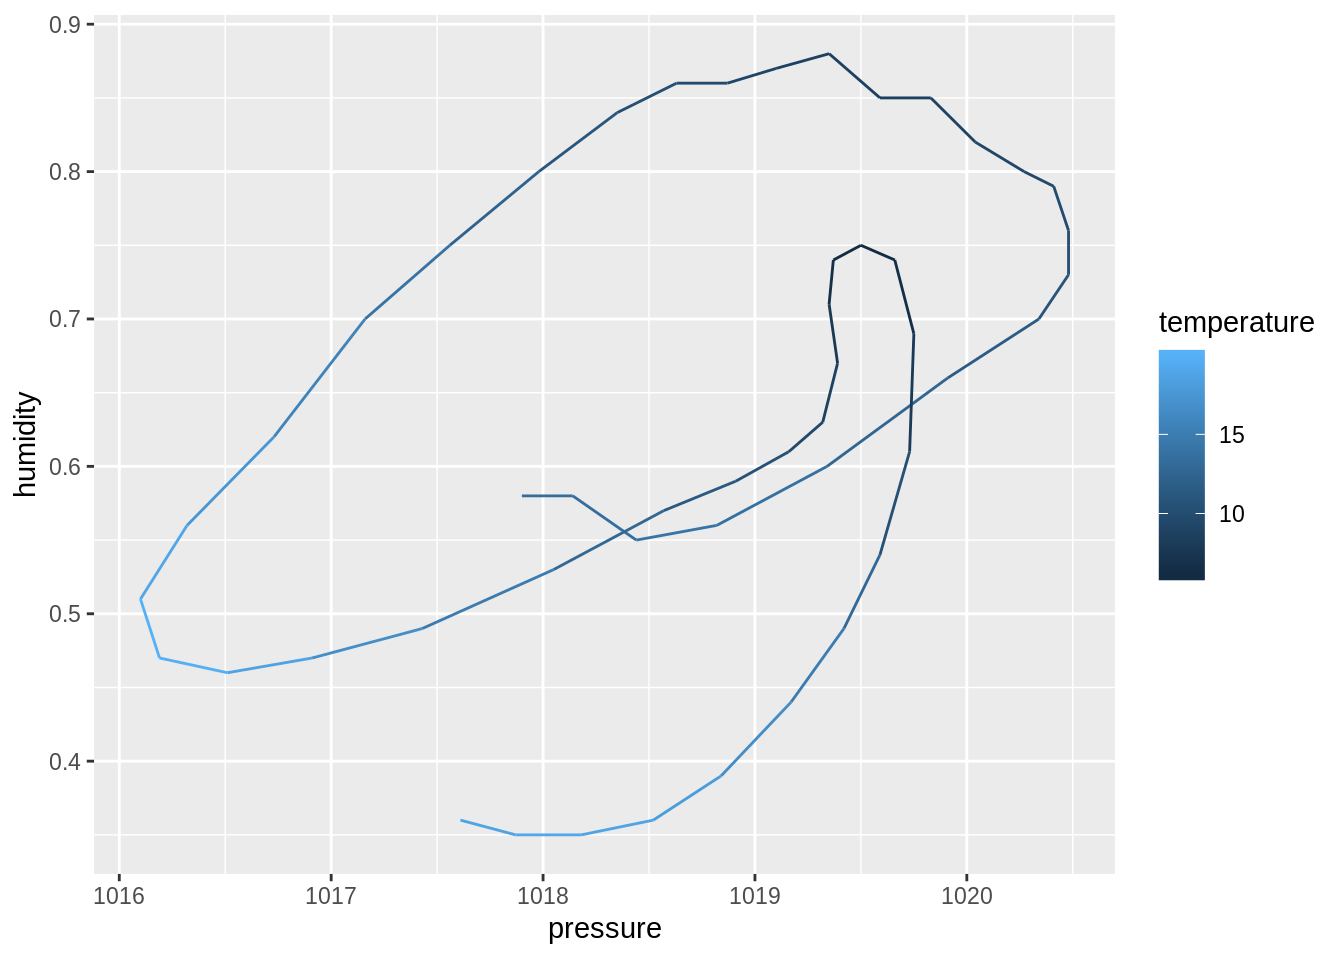
\includegraphics{tidyprog_files/figure-latex/unnamed-chunk-144-1.pdf}

\begin{verbatim}
## 
## $toronto
\end{verbatim}

  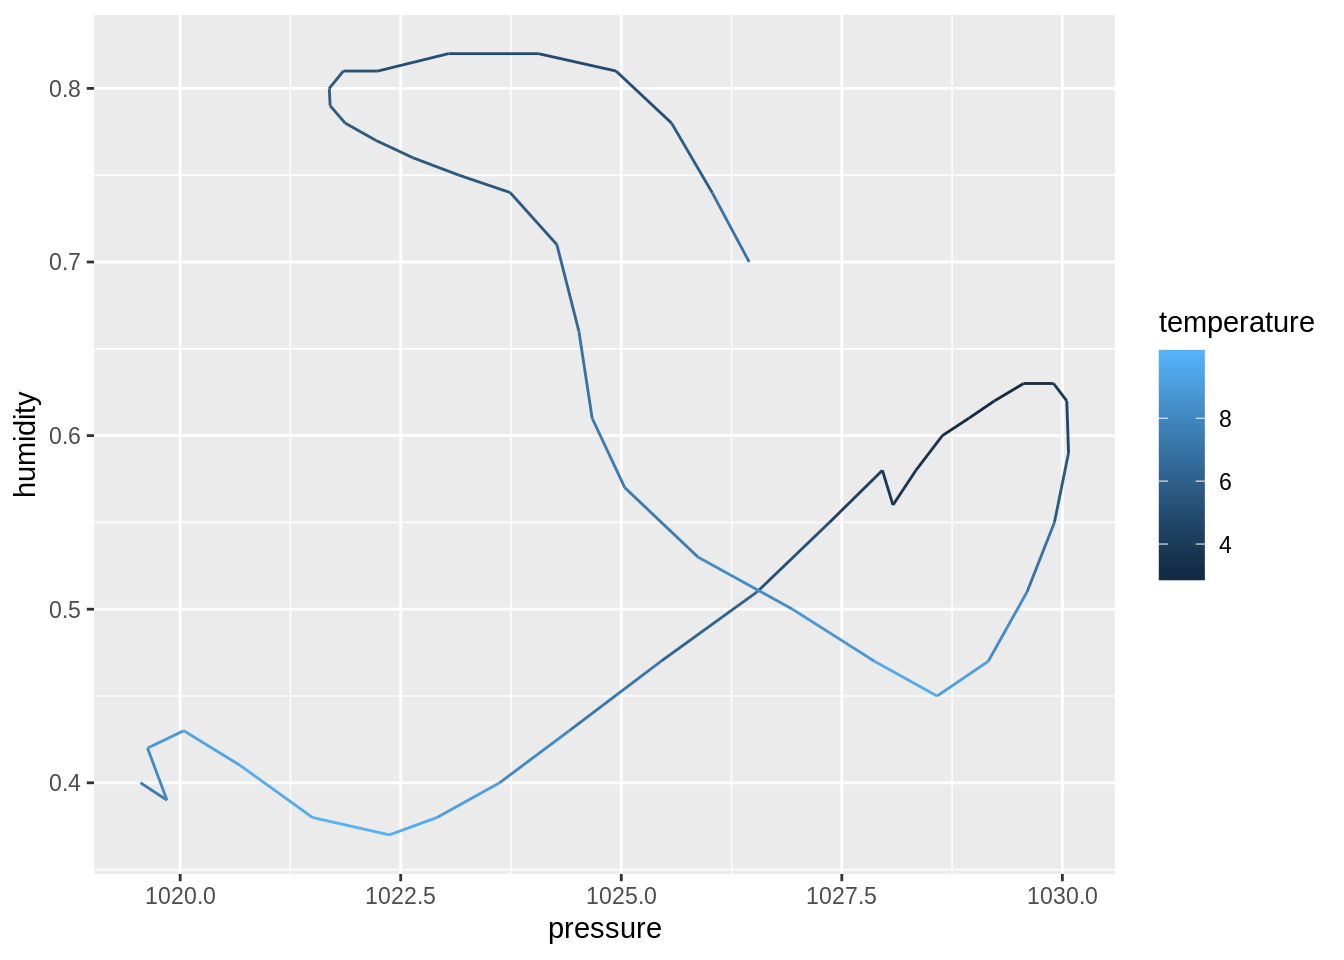
\includegraphics{tidyprog_files/figure-latex/unnamed-chunk-144-2.pdf}

\begin{verbatim}
## 
## $tel_aviv
\end{verbatim}

  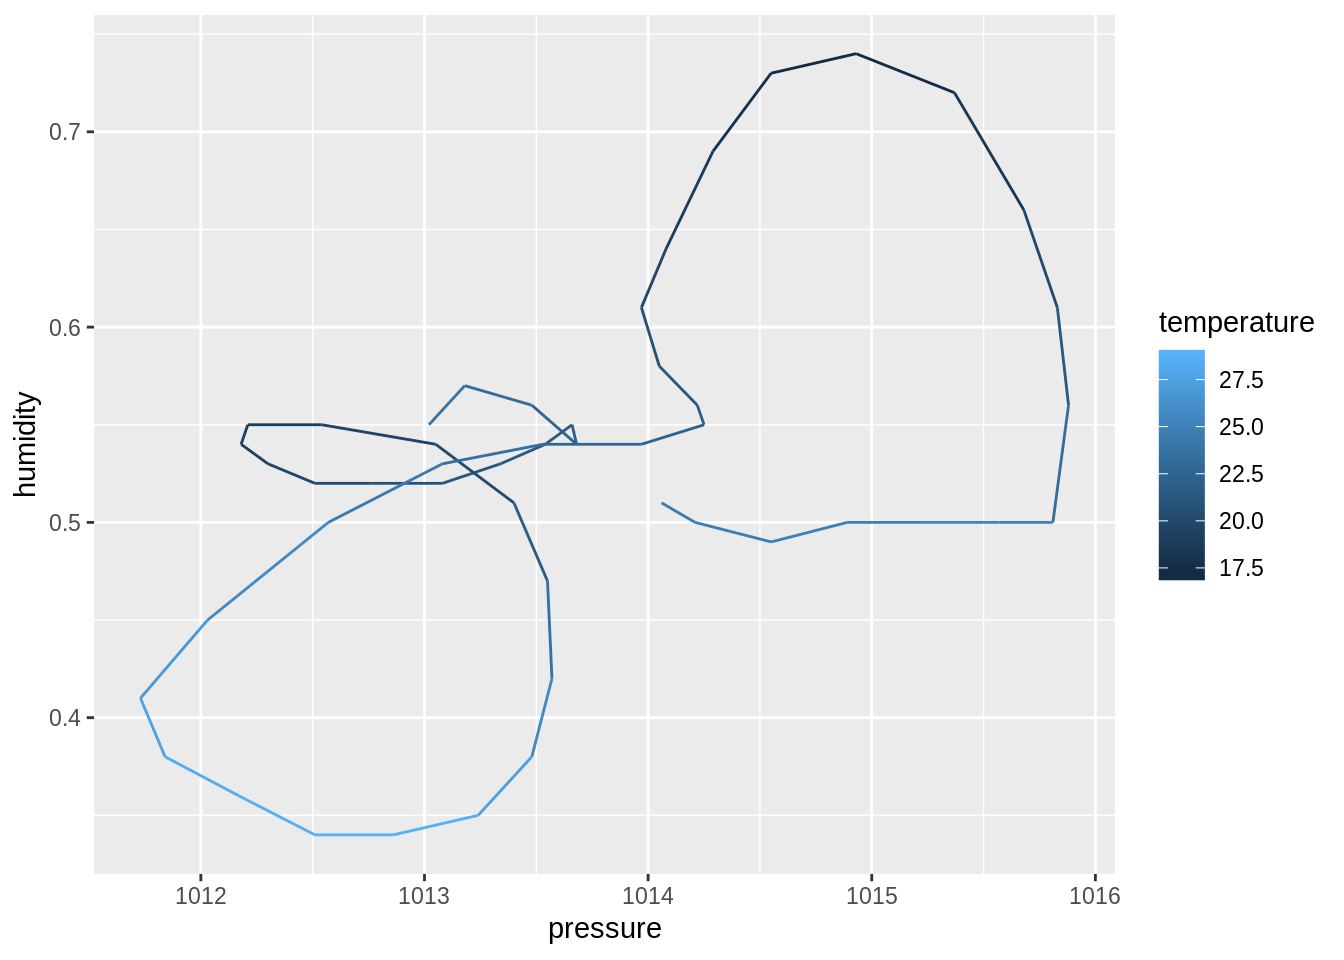
\includegraphics{tidyprog_files/figure-latex/unnamed-chunk-144-3.pdf}

\begin{verbatim}
## 
## $zurich
\end{verbatim}

  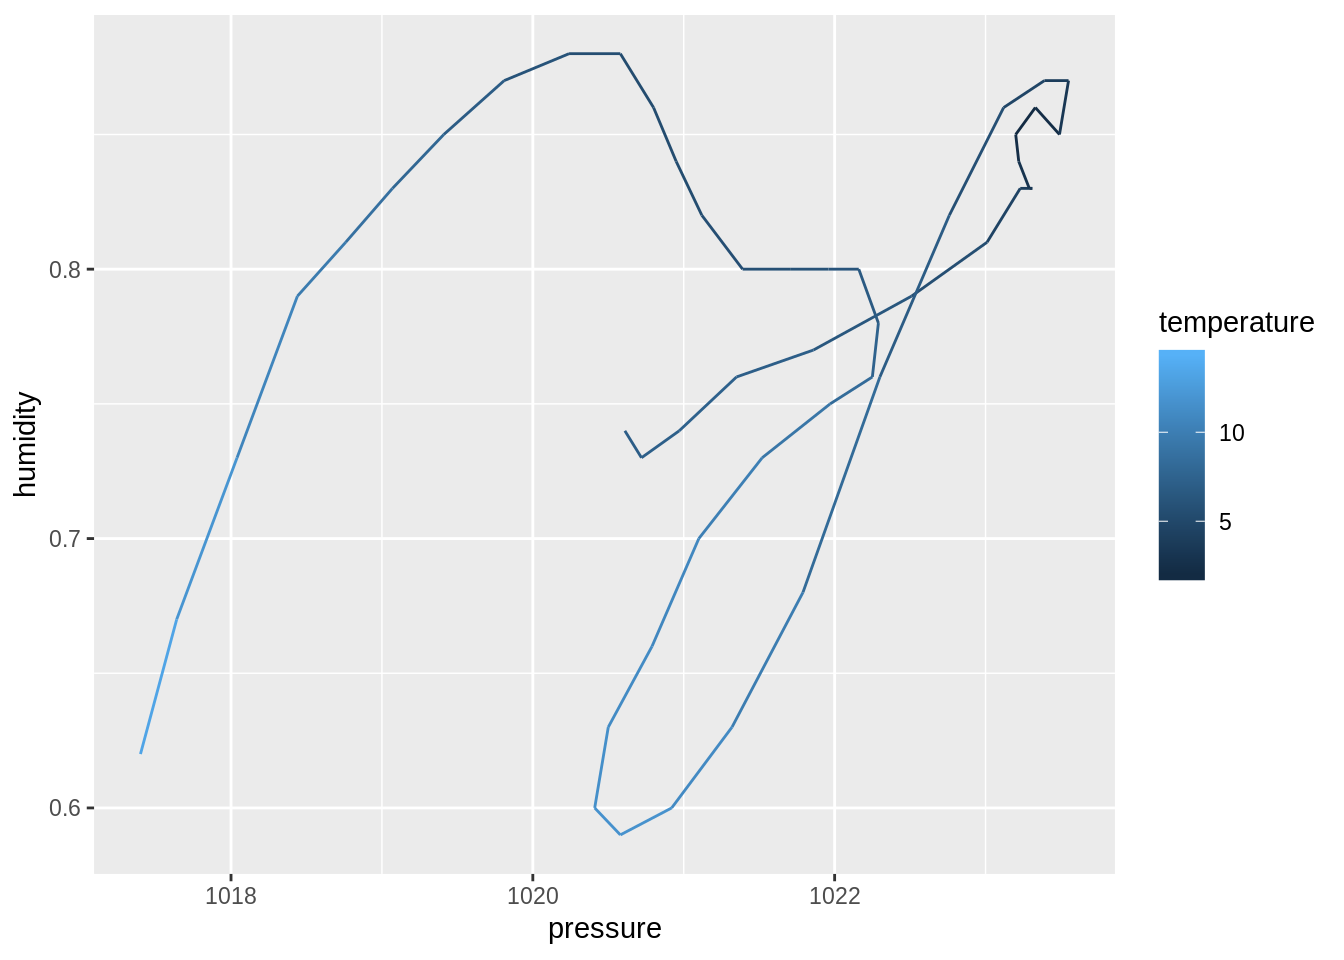
\includegraphics{tidyprog_files/figure-latex/unnamed-chunk-144-4.pdf}
\end{enumerate}

\hypertarget{typed-output}{%
\section{Typed output}\label{typed-output}}

\emph{Click here to show setup code.}

\begin{Shaded}
\begin{Highlighting}[]
\KeywordTok{library}\NormalTok{(tidyverse)}
\KeywordTok{library}\NormalTok{(here)}

\NormalTok{dict <-}\StringTok{ }\NormalTok{readxl}\OperatorTok{::}\KeywordTok{read_excel}\NormalTok{(}\KeywordTok{here}\NormalTok{(}\StringTok{"data/cities.xlsx"}\NormalTok{))}

\NormalTok{input_data <-}
\StringTok{  }\NormalTok{dict }\OperatorTok
\StringTok{  }\KeywordTok{select}\NormalTok{(city_code, weather_filename) }\OperatorTok
\StringTok{  }\KeywordTok{deframe}\NormalTok{() }\OperatorTok
\StringTok{  }\KeywordTok{map}\NormalTok{(}\OperatorTok{~}\StringTok{ }\NormalTok{readxl}\OperatorTok{::}\KeywordTok{read_excel}\NormalTok{(}\KeywordTok{here}\NormalTok{(.)))}
\end{Highlighting}
\end{Shaded}

If we know, what the output of each function call in a \texttt{map()} sequence looks like, we can often call a sub-type of \texttt{map()} to produce a more condensed output.

We start with the named list of tibbles called \texttt{input\_data} from section \protect\hyperlink{map}{``Processing all files''}.

We want to know the number of rows of each tibble in \texttt{input\_data}:

\begin{Shaded}
\begin{Highlighting}[]
\NormalTok{input_data }\OperatorTok
\StringTok{  }\KeywordTok{map}\NormalTok{(}\OperatorTok{~}\StringTok{ }\KeywordTok{nrow}\NormalTok{(.))}
\end{Highlighting}
\end{Shaded}

\begin{verbatim}
## $berlin
## [1] 49
## 
## $toronto
## [1] 49
## 
## $tel_aviv
## [1] 49
## 
## $zurich
## [1] 49
\end{verbatim}

Each time an integer is produced.
Therefore we can call \texttt{map\_int()}, to create a named integer vector:

\begin{Shaded}
\begin{Highlighting}[]
\NormalTok{input_data }\OperatorTok
\StringTok{  }\KeywordTok{map_int}\NormalTok{(}\OperatorTok{~}\StringTok{ }\KeywordTok{nrow}\NormalTok{(.))}
\end{Highlighting}
\end{Shaded}

\begin{verbatim}
##   berlin  toronto tel_aviv   zurich 
##       49       49       49       49
\end{verbatim}

If the output is of type character, use \texttt{map\_chr()}:

\begin{Shaded}
\begin{Highlighting}[]
\NormalTok{input_data }\OperatorTok
\StringTok{  }\KeywordTok{map_chr}\NormalTok{(}\OperatorTok{~}\StringTok{ }\KeywordTok{nrow}\NormalTok{(.))}
\end{Highlighting}
\end{Shaded}

\begin{verbatim}
##   berlin  toronto tel_aviv   zurich 
##     "49"     "49"     "49"     "49"
\end{verbatim}

\begin{Shaded}
\begin{Highlighting}[]
\NormalTok{input_data }\OperatorTok
\StringTok{  }\KeywordTok{map_chr}\NormalTok{(}\OperatorTok{~}\StringTok{ }\KeywordTok{as.character}\NormalTok{(}\KeywordTok{nrow}\NormalTok{(.)))}
\end{Highlighting}
\end{Shaded}

\begin{verbatim}
##   berlin  toronto tel_aviv   zurich 
##     "49"     "49"     "49"     "49"
\end{verbatim}

There are sub-types of the \texttt{map()} function for each atomic type:

\begin{itemize}
\item
  integer: \texttt{map\_int()}
\item
  numeric (double-precision value): \texttt{map\_dbl()}
\item
  character (strings): \texttt{map\_chr()}
\item
  logical (flags): \texttt{map\_lgl()}
\item
  raw (bytes): \texttt{map\_raw()}
\end{itemize}

\hypertarget{exercises-12}{%
\subsection{Exercises}\label{exercises-12}}

\begin{enumerate}
\def\labelenumi{\arabic{enumi}.}
\item
  Explain what happens if you try to use \texttt{map\_dbl()} with the \texttt{dim()} output:

\begin{Shaded}
\begin{Highlighting}[]
\NormalTok{input_data }\OperatorTok\StringTok{ }
\StringTok{  }\KeywordTok{map_dbl}\NormalTok{(dim)}
\end{Highlighting}
\end{Shaded}
\item
  Extract a concise version of the first temperature value for each dataset:

\begin{Shaded}
\begin{Highlighting}[]
\NormalTok{input_data }\OperatorTok\StringTok{ }
\StringTok{  }\KeywordTok{map}\NormalTok{(}\OperatorTok{~}\StringTok{ }\KeywordTok{slice}\NormalTok{(., }\DecValTok{1}\NormalTok{)) }\OperatorTok
\StringTok{  }\KeywordTok{___}\NormalTok{(}\OperatorTok{~}\StringTok{ }\KeywordTok{pull}\NormalTok{(_____))}
\end{Highlighting}
\end{Shaded}

\begin{verbatim}
##   berlin  toronto tel_aviv   zurich 
##    13.43     7.46    23.90     6.96
\end{verbatim}
\item
  Use \texttt{paste0()} to build a textual description for the weather during the observed period in a function. Create a two-column tibble.

\begin{Shaded}
\begin{Highlighting}[]
\NormalTok{summarize_weather <-}\StringTok{ }\NormalTok{_____ \{}
\NormalTok{  ___ }\OperatorTok
\StringTok{    }\KeywordTok{___}\NormalTok{(}
\NormalTok{      _____,}
\NormalTok{      _____,}
\NormalTok{      _____,}
      \DataTypeTok{summary =} \KeywordTok{paste}\NormalTok{(}\KeywordTok{rle}\NormalTok{(summary)}\OperatorTok{$}\NormalTok{values, }\DataTypeTok{collapse =} \StringTok{", then "}\NormalTok{)}
\NormalTok{    )}
\NormalTok{\}}

\NormalTok{describe_weather <-}\StringTok{ }\ControlFlowTok{function}\NormalTok{(weather_summary) \{}
\NormalTok{  weather_summary }\OperatorTok
\StringTok{    }\KeywordTok{mutate}\NormalTok{(}
      \DataTypeTok{text =} \KeywordTok{paste0}\NormalTok{(}
        \StringTok{"We had temperatures between "}\NormalTok{, min_temp, }\StringTok{" and "}\NormalTok{, max_temp, }\StringTok{" °C."}\NormalTok{,}
        \StringTok{"The average humidity was "}\NormalTok{, }\KeywordTok{round}\NormalTok{(mean_humidity }\OperatorTok{*}\StringTok{ }\DecValTok{100}\NormalTok{), }\StringTok{" %. "}\NormalTok{,}
        \StringTok{"The weather was "}\NormalTok{, summary, }\StringTok{"."}
\NormalTok{      )}
\NormalTok{    ) }\OperatorTok\StringTok{ }
\StringTok{    }\KeywordTok{pull}\NormalTok{()}
\NormalTok{\}}

\NormalTok{input_data }\OperatorTok\StringTok{ }
\StringTok{  }\KeywordTok{___}\NormalTok{(___) }\OperatorTok
\StringTok{  }\KeywordTok{___}\NormalTok{(___) }\OperatorTok\StringTok{ }
\StringTok{  }\KeywordTok{___}\NormalTok{()}
\end{Highlighting}
\end{Shaded}

\begin{verbatim}
## # A tibble: 4 x 2
##   name     value                                                           
##   <chr>    <chr>                                                           
## 1 berlin   We had temperatures between 6.14 and 19.98 °C.The average humid~
## 2 toronto  We had temperatures between 3.03 and 9.99 °C.The average humidi~
## 3 tel_aviv We had temperatures between 17.15 and 28.77 °C.The average humi~
## 4 zurich   We had temperatures between 2.01 and 14.3 °C.The average humidi~
\end{verbatim}
\end{enumerate}

\hypertarget{pairwise-iteration-and-nesting}{%
\chapter{Pairwise iteration and nesting}\label{pairwise-iteration-and-nesting}}

This chapter explores iterating over pairs (or generally lists) of vectors of the same length.
The relationship between vectors and data frame columns is especially helpful here, because values in one row of a tibble naturally correspond to accessing the same index in multiple vectors.

This chapter uses the \texttt{manipulated\_data} object from the \protect\hyperlink{map_manip}{``Manipulating all datasets''} section.

\begin{Shaded}
\begin{Highlighting}[]
\KeywordTok{library}\NormalTok{(tidyverse)}
\KeywordTok{library}\NormalTok{(here)}

\NormalTok{dict <-}\StringTok{ }\NormalTok{readxl}\OperatorTok{::}\KeywordTok{read_excel}\NormalTok{(}\KeywordTok{here}\NormalTok{(}\StringTok{"data/cities.xlsx"}\NormalTok{))}

\NormalTok{input_data <-}
\StringTok{  }\NormalTok{dict }\OperatorTok
\StringTok{  }\KeywordTok{select}\NormalTok{(city_code, weather_filename) }\OperatorTok
\StringTok{  }\KeywordTok{deframe}\NormalTok{() }\OperatorTok
\StringTok{  }\KeywordTok{map}\NormalTok{(}\OperatorTok{~}\StringTok{ }\NormalTok{readxl}\OperatorTok{::}\KeywordTok{read_excel}\NormalTok{(}\KeywordTok{here}\NormalTok{(.)))}

\NormalTok{find_good_times <-}\StringTok{ }\ControlFlowTok{function}\NormalTok{(data) \{}
\NormalTok{  data }\OperatorTok
\StringTok{    }\KeywordTok{select}\NormalTok{(time, }\KeywordTok{contains}\NormalTok{(}\StringTok{"emperature"}\NormalTok{)) }\OperatorTok
\StringTok{    }\KeywordTok{filter}\NormalTok{(temperature }\OperatorTok{>=}\StringTok{ }\DecValTok{14}\NormalTok{)}
\NormalTok{\}}

\NormalTok{good_times <-}
\StringTok{  }\NormalTok{input_data }\OperatorTok
\StringTok{  }\KeywordTok{map}\NormalTok{(find_good_times)}

\NormalTok{good_times}
\end{Highlighting}
\end{Shaded}

\begin{verbatim}
## $berlin
## # A tibble: 16 x 3
##   time                temperature apparentTemperature
##   <dttm>                    <dbl>               <dbl>
## 1 2019-04-28 17:00:00        14.1                14.1
## 2 2019-04-29 12:00:00        15.6                15.6
## 3 2019-04-29 13:00:00        17.4                17.4
## # ... with 13 more rows
## 
## $toronto
## # A tibble: 0 x 3
## # ... with 3 variables: time <dttm>, temperature <dbl>,
## #   apparentTemperature <dbl>
## 
## $tel_aviv
## # A tibble: 49 x 3
##   time                temperature apparentTemperature
##   <dttm>                    <dbl>               <dbl>
## 1 2019-04-28 15:00:00        23.9                23.9
## 2 2019-04-28 16:00:00        23.1                23.1
## 3 2019-04-28 17:00:00        22.4                22.4
## # ... with 46 more rows
## 
## $zurich
## # A tibble: 1 x 3
##   time                temperature apparentTemperature
##   <dttm>                    <dbl>               <dbl>
## 1 2019-04-30 15:00:00        14.3                14.3
\end{verbatim}

\hypertarget{manipulating-pairwise}{%
\section{Manipulating pairwise}\label{manipulating-pairwise}}

Here we discuss cases when you want to iterate through two lists (of the same length) in parallel and use each value pair as two of the input parameters of a function.

We first prepare a list of future output filenames:

\begin{Shaded}
\begin{Highlighting}[]
\NormalTok{output_filenames <-}\StringTok{ }\KeywordTok{tempfile}\NormalTok{(}\KeywordTok{names}\NormalTok{(good_times), }\DataTypeTok{fileext =} \StringTok{".csv"}\NormalTok{)}
\NormalTok{output_filenames}
\end{Highlighting}
\end{Shaded}

\begin{verbatim}
## [1] "/tmp/RtmpLeqSdR/berlin2d3e6781b213.csv"  
## [2] "/tmp/RtmpLeqSdR/toronto2d3e4bc709e0.csv" 
## [3] "/tmp/RtmpLeqSdR/tel_aviv2d3e5734c1fa.csv"
## [4] "/tmp/RtmpLeqSdR/zurich2d3e69d5cf1e.csv"
\end{verbatim}

We want to use \texttt{readr::write\_csv()} to write each tibble into the respective file.
\texttt{write\_csv()} needs at least 2 arguments: the tibble itself and the path to the filename.
For illustration, we implement a file-centric wrapper function that takes the file name as first argument and also prints a message every time a file is written.
We use \texttt{map2()} to handle this:

\begin{Shaded}
\begin{Highlighting}[]
\NormalTok{process_csv <-}\StringTok{ }\ControlFlowTok{function}\NormalTok{(file, data) \{}
\NormalTok{  readr}\OperatorTok{::}\KeywordTok{write_csv}\NormalTok{(data, file)}
  \KeywordTok{message}\NormalTok{(}\StringTok{"Writing "}\NormalTok{, file)}
  \KeywordTok{invisible}\NormalTok{(file)}
\NormalTok{\}}

\KeywordTok{map2}\NormalTok{(good_times, output_filenames, }\OperatorTok{~}\StringTok{ }\KeywordTok{process_csv}\NormalTok{(..}\DecValTok{2}\NormalTok{, ..}\DecValTok{1}\NormalTok{))}
\end{Highlighting}
\end{Shaded}

\begin{verbatim}
## Writing /tmp/RtmpLeqSdR/berlin2d3e6781b213.csv
\end{verbatim}

\begin{verbatim}
## Writing /tmp/RtmpLeqSdR/toronto2d3e4bc709e0.csv
\end{verbatim}

\begin{verbatim}
## Writing /tmp/RtmpLeqSdR/tel_aviv2d3e5734c1fa.csv
\end{verbatim}

\begin{verbatim}
## Writing /tmp/RtmpLeqSdR/zurich2d3e69d5cf1e.csv
\end{verbatim}

\begin{verbatim}
## $berlin
## [1] "/tmp/RtmpLeqSdR/berlin2d3e6781b213.csv"
## 
## $toronto
## [1] "/tmp/RtmpLeqSdR/toronto2d3e4bc709e0.csv"
## 
## $tel_aviv
## [1] "/tmp/RtmpLeqSdR/tel_aviv2d3e5734c1fa.csv"
## 
## $zurich
## [1] "/tmp/RtmpLeqSdR/zurich2d3e69d5cf1e.csv"
\end{verbatim}

\begin{Shaded}
\begin{Highlighting}[]
\KeywordTok{invisible}\NormalTok{(}\KeywordTok{map2}\NormalTok{(good_times, output_filenames, }\OperatorTok{~}\StringTok{ }\KeywordTok{process_csv}\NormalTok{(..}\DecValTok{2}\NormalTok{, ..}\DecValTok{1}\NormalTok{)))}
\end{Highlighting}
\end{Shaded}

\begin{verbatim}
## Writing /tmp/RtmpLeqSdR/berlin2d3e6781b213.csv
\end{verbatim}

\begin{verbatim}
## Writing /tmp/RtmpLeqSdR/toronto2d3e4bc709e0.csv
\end{verbatim}

\begin{verbatim}
## Writing /tmp/RtmpLeqSdR/tel_aviv2d3e5734c1fa.csv
\end{verbatim}

\begin{verbatim}
## Writing /tmp/RtmpLeqSdR/zurich2d3e69d5cf1e.csv
\end{verbatim}

Because \texttt{process\_csv()} returns the file name, it is available as output.
Since we are just interested in the side-effects of \texttt{write\_csv()} and not in the displayed output, we can use the related function \texttt{walk2()}.

\begin{Shaded}
\begin{Highlighting}[]
\KeywordTok{walk2}\NormalTok{(good_times, output_filenames, }\OperatorTok{~}\StringTok{ }\KeywordTok{process_csv}\NormalTok{(..}\DecValTok{2}\NormalTok{, ..}\DecValTok{1}\NormalTok{))}
\end{Highlighting}
\end{Shaded}

\begin{verbatim}
## Writing /tmp/RtmpLeqSdR/berlin2d3e6781b213.csv
\end{verbatim}

\begin{verbatim}
## Writing /tmp/RtmpLeqSdR/toronto2d3e4bc709e0.csv
\end{verbatim}

\begin{verbatim}
## Writing /tmp/RtmpLeqSdR/tel_aviv2d3e5734c1fa.csv
\end{verbatim}

\begin{verbatim}
## Writing /tmp/RtmpLeqSdR/zurich2d3e69d5cf1e.csv
\end{verbatim}

\begin{Shaded}
\begin{Highlighting}[]
\KeywordTok{print}\NormalTok{(}\KeywordTok{walk2}\NormalTok{(good_times, output_filenames, }\OperatorTok{~}\StringTok{ }\KeywordTok{process_csv}\NormalTok{(..}\DecValTok{2}\NormalTok{, ..}\DecValTok{1}\NormalTok{)))}
\end{Highlighting}
\end{Shaded}

\begin{verbatim}
## Writing /tmp/RtmpLeqSdR/berlin2d3e6781b213.csv
\end{verbatim}

\begin{verbatim}
## Writing /tmp/RtmpLeqSdR/toronto2d3e4bc709e0.csv
\end{verbatim}

\begin{verbatim}
## Writing /tmp/RtmpLeqSdR/tel_aviv2d3e5734c1fa.csv
\end{verbatim}

\begin{verbatim}
## Writing /tmp/RtmpLeqSdR/zurich2d3e69d5cf1e.csv
\end{verbatim}

\begin{verbatim}
## $berlin
## # A tibble: 16 x 3
##   time                temperature apparentTemperature
##   <dttm>                    <dbl>               <dbl>
## 1 2019-04-28 17:00:00        14.1                14.1
## 2 2019-04-29 12:00:00        15.6                15.6
## 3 2019-04-29 13:00:00        17.4                17.4
## # ... with 13 more rows
## 
## $toronto
## # A tibble: 0 x 3
## # ... with 3 variables: time <dttm>, temperature <dbl>,
## #   apparentTemperature <dbl>
## 
## $tel_aviv
## # A tibble: 49 x 3
##   time                temperature apparentTemperature
##   <dttm>                    <dbl>               <dbl>
## 1 2019-04-28 15:00:00        23.9                23.9
## 2 2019-04-28 16:00:00        23.1                23.1
## 3 2019-04-28 17:00:00        22.4                22.4
## # ... with 46 more rows
## 
## $zurich
## # A tibble: 1 x 3
##   time                temperature apparentTemperature
##   <dttm>                    <dbl>               <dbl>
## 1 2019-04-30 15:00:00        14.3                14.3
\end{verbatim}

\texttt{walk2()} returns its first argument so that it can be used in a pipe.

\hypertarget{exercises-13}{%
\subsection{Exercises}\label{exercises-13}}

\begin{enumerate}
\def\labelenumi{\arabic{enumi}.}
\item
  What does the following code display?

\begin{Shaded}
\begin{Highlighting}[]
\NormalTok{good_times }\OperatorTok\StringTok{ }
\StringTok{  }\KeywordTok{walk2}\NormalTok{(output_filenames, }\OperatorTok{~}\StringTok{ }\NormalTok{readr}\OperatorTok{::}\KeywordTok{write_csv}\NormalTok{(..}\DecValTok{1}\NormalTok{, ..}\DecValTok{2}\NormalTok{)) }\OperatorTok\StringTok{ }
\StringTok{  }\KeywordTok{map_int}\NormalTok{(nrow)}
\end{Highlighting}
\end{Shaded}
\end{enumerate}

\hypertarget{mut_map}{%
\section{Moving to tibble-land}\label{mut_map}}

\emph{Click here to show setup code.}

\begin{Shaded}
\begin{Highlighting}[]
\KeywordTok{library}\NormalTok{(tidyverse)}
\KeywordTok{library}\NormalTok{(here)}

\NormalTok{dict <-}\StringTok{ }\NormalTok{readxl}\OperatorTok{::}\KeywordTok{read_excel}\NormalTok{(}\KeywordTok{here}\NormalTok{(}\StringTok{"data/cities.xlsx"}\NormalTok{))}

\NormalTok{input_data <-}
\StringTok{  }\NormalTok{dict }\OperatorTok
\StringTok{  }\KeywordTok{select}\NormalTok{(city_code, weather_filename) }\OperatorTok
\StringTok{  }\KeywordTok{deframe}\NormalTok{() }\OperatorTok
\StringTok{  }\KeywordTok{map}\NormalTok{(}\OperatorTok{~}\StringTok{ }\NormalTok{readxl}\OperatorTok{::}\KeywordTok{read_excel}\NormalTok{(}\KeywordTok{here}\NormalTok{(.)))}

\NormalTok{find_good_times <-}\StringTok{ }\ControlFlowTok{function}\NormalTok{(data) \{}
\NormalTok{  data }\OperatorTok
\StringTok{    }\KeywordTok{select}\NormalTok{(time, }\KeywordTok{contains}\NormalTok{(}\StringTok{"emperature"}\NormalTok{)) }\OperatorTok
\StringTok{    }\KeywordTok{filter}\NormalTok{(temperature }\OperatorTok{>=}\StringTok{ }\DecValTok{14}\NormalTok{)}
\NormalTok{\}}

\NormalTok{good_times <-}
\StringTok{  }\NormalTok{input_data }\OperatorTok
\StringTok{  }\KeywordTok{map}\NormalTok{(find_good_times)}
\end{Highlighting}
\end{Shaded}

How to combine the abilities of \texttt{map()} \& co., which work on vectors and lists, with our commonly used data structure, the tibble?

We start with the named list of tibbles called \texttt{input\_data} from section \protect\hyperlink{map}{``Processing all files''} and with \texttt{dict} from section \protect\hyperlink{names}{``Named vectors and two-column tibbles''}.

Calling \texttt{enframe()} to produce a data frame from \texttt{input\_data} leads to a maybe at first surprising, but oftentimes useful result:

\begin{Shaded}
\begin{Highlighting}[]
\NormalTok{nested_input_data <-}
\StringTok{  }\NormalTok{input_data }\OperatorTok
\StringTok{  }\KeywordTok{enframe}\NormalTok{()}

\NormalTok{nested_input_data}
\end{Highlighting}
\end{Shaded}

\begin{verbatim}
## # A tibble: 4 x 2
##   name     value             
##   <chr>    <list>            
## 1 berlin   <tibble [49 x 18]>
## 2 toronto  <tibble [49 x 18]>
## 3 tel_aviv <tibble [49 x 17]>
## 4 zurich   <tibble [49 x 18]>
\end{verbatim}

This is because lists are also vectors.
In our case each list entry contains a tibble, which can be ``nested'' into each entry of column \texttt{value}.

Starting with the tibble \texttt{dict} we can see how \texttt{dpylr::mutate()} and \texttt{map()} can nicely work together to produce a somewhat similar result:

\begin{Shaded}
\begin{Highlighting}[]
\NormalTok{dict }\OperatorTok
\StringTok{  }\KeywordTok{select}\NormalTok{(city_code, weather_filename) }\OperatorTok
\StringTok{  }\KeywordTok{mutate}\NormalTok{(}
    \DataTypeTok{data =} \KeywordTok{map}\NormalTok{(weather_filename, }\OperatorTok{~}\StringTok{ }\NormalTok{readxl}\OperatorTok{::}\KeywordTok{read_excel}\NormalTok{(}\KeywordTok{here}\NormalTok{(.)))}
\NormalTok{  )}
\end{Highlighting}
\end{Shaded}

\begin{verbatim}
## # A tibble: 4 x 3
##   city_code weather_filename           data              
##   <chr>     <chr>                      <list>            
## 1 berlin    data/weather/berlin.xlsx   <tibble [49 x 18]>
## 2 toronto   data/weather/toronto.xlsx  <tibble [49 x 18]>
## 3 tel_aviv  data/weather/tel_aviv.xlsx <tibble [49 x 17]>
## 4 zurich    data/weather/zurich.xlsx   <tibble [49 x 18]>
\end{verbatim}

This works because \texttt{R} interprets columns of tibbles as vectors, which can be fed to \texttt{map()}.
To simplify the \texttt{map()} call, we create an intermediate column:

\begin{Shaded}
\begin{Highlighting}[]
\NormalTok{dict }\OperatorTok
\StringTok{  }\KeywordTok{select}\NormalTok{(city_code, weather_filename) }\OperatorTok
\StringTok{  }\KeywordTok{mutate}\NormalTok{(}\DataTypeTok{path =} \KeywordTok{here}\NormalTok{(weather_filename)) }\OperatorTok
\StringTok{  }\KeywordTok{mutate}\NormalTok{(}\DataTypeTok{data =} \KeywordTok{map}\NormalTok{(path, readxl}\OperatorTok{::}\NormalTok{read_excel))}
\end{Highlighting}
\end{Shaded}

\begin{verbatim}
## # A tibble: 4 x 4
##   city_code weather_filename      path                           data      
##   <chr>     <chr>                 <chr>                          <list>    
## 1 berlin    data/weather/berlin.~ /home/travis/build/krlmlr/tid~ <tibble [~
## 2 toronto   data/weather/toronto~ /home/travis/build/krlmlr/tid~ <tibble [~
## 3 tel_aviv  data/weather/tel_avi~ /home/travis/build/krlmlr/tid~ <tibble [~
## 4 zurich    data/weather/zurich.~ /home/travis/build/krlmlr/tid~ <tibble [~
\end{verbatim}

Staying in ``tibble-land'' as long as possible helps retaining other important components of the data you are processing, so that you can keep using familiar data transformation tools.

\begin{Shaded}
\begin{Highlighting}[]
\NormalTok{dict_data <-}
\StringTok{  }\NormalTok{dict }\OperatorTok
\StringTok{  }\KeywordTok{mutate}\NormalTok{(}
    \DataTypeTok{data =} \KeywordTok{map}\NormalTok{(weather_filename, }\OperatorTok{~}\StringTok{ }\NormalTok{readxl}\OperatorTok{::}\KeywordTok{read_excel}\NormalTok{(}\KeywordTok{here}\NormalTok{(.))),}
    \DataTypeTok{rows =} \KeywordTok{map_int}\NormalTok{(data, nrow),}
\NormalTok{  ) }\OperatorTok
\StringTok{  }\KeywordTok{select}\NormalTok{(}\OperatorTok{-}\NormalTok{weather_filename)}
\NormalTok{dict_data}
\end{Highlighting}
\end{Shaded}

\begin{verbatim}
## # A tibble: 4 x 6
##   city_code name        lng   lat data                rows
##   <chr>     <chr>     <dbl> <dbl> <list>             <int>
## 1 berlin    Berlin    13.4   52.5 <tibble [49 x 18]>    49
## 2 toronto   Toronto  -79.4   43.7 <tibble [49 x 18]>    49
## 3 tel_aviv  Tel Aviv  34.8   32.1 <tibble [49 x 17]>    49
## 4 zurich    Zürich     8.54  47.4 <tibble [49 x 18]>    49
\end{verbatim}

This pattern can also be used with the \texttt{map2()} family of functions:

\begin{Shaded}
\begin{Highlighting}[]
\NormalTok{dict_data_with_desc <-}
\StringTok{  }\NormalTok{dict_data }\OperatorTok
\StringTok{  }\KeywordTok{mutate}\NormalTok{(}
    \DataTypeTok{desc =} \KeywordTok{map2_chr}\NormalTok{(}
\NormalTok{      name, rows,}
      \OperatorTok{~}\StringTok{ }\KeywordTok{paste0}\NormalTok{(..}\DecValTok{2}\NormalTok{, }\StringTok{" rows in data for "}\NormalTok{, ..}\DecValTok{1}\NormalTok{)}
\NormalTok{    )}
\NormalTok{  )}
\end{Highlighting}
\end{Shaded}

Because \texttt{mutate()} always appends to the end, the most recently added column can always be accessed with \texttt{pull()}:

\begin{Shaded}
\begin{Highlighting}[]
\NormalTok{dict_data_with_desc }\OperatorTok
\StringTok{  }\KeywordTok{pull}\NormalTok{()}
\end{Highlighting}
\end{Shaded}

\begin{verbatim}
## [1] "49 rows in data for Berlin"   "49 rows in data for Toronto" 
## [3] "49 rows in data for Tel Aviv" "49 rows in data for Zürich"
\end{verbatim}

More generally, \texttt{pmap()} supports functions with an arbitrary number of arguments:

\begin{Shaded}
\begin{Highlighting}[]
\NormalTok{dict_data }\OperatorTok
\StringTok{  }\KeywordTok{mutate}\NormalTok{(}
    \DataTypeTok{cols =} \KeywordTok{map_int}\NormalTok{(data, ncol),}
    \DataTypeTok{desc =} \KeywordTok{pmap_chr}\NormalTok{(}
      \KeywordTok{list}\NormalTok{(name, rows, cols),}
      \OperatorTok{~}\StringTok{ }\KeywordTok{paste0}\NormalTok{(..}\DecValTok{2}\NormalTok{, }\StringTok{" rows and "}\NormalTok{, ..}\DecValTok{3}\NormalTok{, }\StringTok{" cols in data for "}\NormalTok{, ..}\DecValTok{1}\NormalTok{)}
\NormalTok{    )}
\NormalTok{  )}
\end{Highlighting}
\end{Shaded}

\begin{verbatim}
## # A tibble: 4 x 8
##   city_code name       lng   lat data        rows  cols desc               
##   <chr>     <chr>    <dbl> <dbl> <list>     <int> <int> <chr>              
## 1 berlin    Berlin   13.4   52.5 <tibble [~    49    18 49 rows and 18 col~
## 2 toronto   Toronto -79.4   43.7 <tibble [~    49    18 49 rows and 18 col~
## 3 tel_aviv  Tel Av~  34.8   32.1 <tibble [~    49    17 49 rows and 17 col~
## 4 zurich    Zürich    8.54  47.4 <tibble [~    49    18 49 rows and 18 col~
\end{verbatim}

\hypertarget{exercises-14}{%
\subsection{Exercises}\label{exercises-14}}

\begin{enumerate}
\def\labelenumi{\arabic{enumi}.}
\item
  The \texttt{imap()} family of functions iterates over a vector and its names:

\begin{Shaded}
\begin{Highlighting}[]
\NormalTok{input_data }\OperatorTok\StringTok{ }
\StringTok{  }\KeywordTok{imap_chr}\NormalTok{(}\OperatorTok{~}\StringTok{ }\KeywordTok{paste0}\NormalTok{(.y, }\StringTok{": "}\NormalTok{, }\KeywordTok{nrow}\NormalTok{(.x), }\StringTok{" rows"}\NormalTok{))}
\end{Highlighting}
\end{Shaded}

\begin{verbatim}
##              berlin             toronto            tel_aviv 
##   "berlin: 49 rows"  "toronto: 49 rows" "tel_aviv: 49 rows" 
##              zurich 
##   "zurich: 49 rows"
\end{verbatim}

  Implement the same functionality using \texttt{map2()} inside a \texttt{mutate()}, and \texttt{enframe()}:

\begin{Shaded}
\begin{Highlighting}[]
\NormalTok{good_times }\OperatorTok
\StringTok{  }\KeywordTok{___}\NormalTok{() }\OperatorTok
\StringTok{  }\KeywordTok{mutate}\NormalTok{(}\DataTypeTok{___ =} \KeywordTok{map2}\NormalTok{()) }\OperatorTok
\StringTok{  }\KeywordTok{deframe}\NormalTok{()}
\end{Highlighting}
\end{Shaded}
\end{enumerate}

\hypertarget{nest}{%
\section{Nesting and unnesting}\label{nest}}

\emph{Click here to show setup code.}

\begin{Shaded}
\begin{Highlighting}[]
\KeywordTok{library}\NormalTok{(tidyverse)}
\KeywordTok{library}\NormalTok{(here)}

\NormalTok{dict <-}\StringTok{ }\NormalTok{readxl}\OperatorTok{::}\KeywordTok{read_excel}\NormalTok{(}\KeywordTok{here}\NormalTok{(}\StringTok{"data/cities.xlsx"}\NormalTok{))}

\NormalTok{dict_data <-}
\StringTok{  }\NormalTok{dict }\OperatorTok
\StringTok{  }\KeywordTok{mutate}\NormalTok{(}\DataTypeTok{data =} \KeywordTok{map}\NormalTok{(weather_filename, }\OperatorTok{~}\StringTok{ }\NormalTok{readxl}\OperatorTok{::}\KeywordTok{read_excel}\NormalTok{(}\KeywordTok{here}\NormalTok{(.)))) }\OperatorTok
\StringTok{  }\KeywordTok{select}\NormalTok{(}\OperatorTok{-}\NormalTok{weather_filename)}
\end{Highlighting}
\end{Shaded}

How to work with nested data?

We start with the tibble \texttt{dict\_data} from section \protect\hyperlink{mut_map}{``Moving to tibble-land''}, which includes the nested tibbles in its column \texttt{data}.

If we want to actually look at the data we can directly use \texttt{tidyr::unnest()} on the whole tibble, which by default acts on all list-columns.
This expands our tibble by repeating the formerly unnested column entries as many times, as each nested tibble has rows:

\begin{Shaded}
\begin{Highlighting}[]
\NormalTok{dict_data }\OperatorTok
\StringTok{  }\KeywordTok{unnest}\NormalTok{()}
\end{Highlighting}
\end{Shaded}

\begin{verbatim}
## # A tibble: 196 x 22
##   city_code name    lng   lat time                summary icon 
##   <chr>     <chr> <dbl> <dbl> <dttm>              <chr>   <chr>
## 1 berlin    Berl~  13.4  52.5 2019-04-28 15:00:00 Mostly~ part~
## 2 berlin    Berl~  13.4  52.5 2019-04-28 16:00:00 Mostly~ part~
## 3 berlin    Berl~  13.4  52.5 2019-04-28 17:00:00 Mostly~ part~
## # ... with 193 more rows, and 15 more variables: precipIntensity <dbl>,
## #   precipProbability <dbl>, temperature <dbl>, apparentTemperature <dbl>,
## #   dewPoint <dbl>, humidity <dbl>, pressure <dbl>, windSpeed <dbl>,
## #   windGust <dbl>, windBearing <dbl>, cloudCover <dbl>, uvIndex <dbl>,
## #   visibility <dbl>, ozone <dbl>, precipType <chr>
\end{verbatim}

This is very similar to \texttt{bind\_rows()} of the \texttt{data} column.

\begin{Shaded}
\begin{Highlighting}[]
\NormalTok{dict_data }\OperatorTok
\StringTok{  }\KeywordTok{pull}\NormalTok{(data) }\OperatorTok
\StringTok{  }\KeywordTok{bind_rows}\NormalTok{()}
\end{Highlighting}
\end{Shaded}

\begin{verbatim}
## # A tibble: 196 x 18
##   time                summary icon  precipIntensity precipProbabili~
##   <dttm>              <chr>   <chr>           <dbl>            <dbl>
## 1 2019-04-28 15:00:00 Mostly~ part~               0                0
## 2 2019-04-28 16:00:00 Mostly~ part~               0                0
## 3 2019-04-28 17:00:00 Mostly~ part~               0                0
## # ... with 193 more rows, and 13 more variables: temperature <dbl>,
## #   apparentTemperature <dbl>, dewPoint <dbl>, humidity <dbl>,
## #   pressure <dbl>, windSpeed <dbl>, windGust <dbl>, windBearing <dbl>,
## #   cloudCover <dbl>, uvIndex <dbl>, visibility <dbl>, ozone <dbl>,
## #   precipType <chr>
\end{verbatim}

\begin{Shaded}
\begin{Highlighting}[]
\NormalTok{check_columns_same <-}\StringTok{ }\ControlFlowTok{function}\NormalTok{(x, y) \{}
  \KeywordTok{stopifnot}\NormalTok{(}\KeywordTok{identical}\NormalTok{(}\KeywordTok{colnames}\NormalTok{(x), }\KeywordTok{colnames}\NormalTok{(y)))}
\NormalTok{\}}

\NormalTok{bind_rows <-}\StringTok{ }\ControlFlowTok{function}\NormalTok{(data_frames) \{}
  \CommentTok{# Called for the side effect}
  \KeywordTok{reduce}\NormalTok{(data_frames, check_columns_same)}

\NormalTok{  dplyr}\OperatorTok{::}\KeywordTok{bind_rows}\NormalTok{(data_frames)}
\NormalTok{\}}

\KeywordTok{try}\NormalTok{(}
\NormalTok{  dict_data }\OperatorTok
\StringTok{    }\KeywordTok{pull}\NormalTok{(data) }\OperatorTok
\StringTok{    }\KeywordTok{bind_rows}\NormalTok{()}
\NormalTok{)}
\end{Highlighting}
\end{Shaded}

\begin{verbatim}
## Error in fn(out, elt, ...) : 
##   identical(colnames(x), colnames(y)) is not TRUE
\end{verbatim}

Data flattened in this way is useful if the parts can be combined naturally into a larger dataset.
Iterating over columns in the nested view corresponds to grouped operations in the flat view.

\begin{Shaded}
\begin{Highlighting}[]
\NormalTok{dict_data }\OperatorTok
\StringTok{  }\KeywordTok{mutate}\NormalTok{(}\DataTypeTok{n =} \KeywordTok{map_int}\NormalTok{(data, nrow)) }\OperatorTok
\StringTok{  }\KeywordTok{select}\NormalTok{(}\OperatorTok{-}\NormalTok{data)}
\end{Highlighting}
\end{Shaded}

\begin{verbatim}
## # A tibble: 4 x 5
##   city_code name        lng   lat     n
##   <chr>     <chr>     <dbl> <dbl> <int>
## 1 berlin    Berlin    13.4   52.5    49
## 2 toronto   Toronto  -79.4   43.7    49
## 3 tel_aviv  Tel Aviv  34.8   32.1    49
## 4 zurich    Zürich     8.54  47.4    49
\end{verbatim}

\begin{Shaded}
\begin{Highlighting}[]
\NormalTok{dict_data }\OperatorTok
\StringTok{  }\KeywordTok{unnest}\NormalTok{() }\OperatorTok
\StringTok{  }\KeywordTok{count}\NormalTok{(name)}
\end{Highlighting}
\end{Shaded}

\begin{verbatim}
## # A tibble: 4 x 2
##   name         n
##   <chr>    <int>
## 1 Berlin      49
## 2 Tel Aviv    49
## 3 Toronto     49
## 4 Zürich      49
\end{verbatim}

Inversely, if you want to have a more condensed view of your data, you can nest again.
By default, the function \texttt{tidyr::nest()} will nest all data.
Therefore it is often useful to tell it, which columns to ignore:

\begin{Shaded}
\begin{Highlighting}[]
\NormalTok{dict_data }\OperatorTok
\StringTok{  }\KeywordTok{unnest}\NormalTok{() }\OperatorTok
\StringTok{  }\KeywordTok{nest}\NormalTok{(}\OperatorTok{-}\NormalTok{city_code, }\OperatorTok{-}\NormalTok{name, }\OperatorTok{-}\NormalTok{lng, }\OperatorTok{-}\NormalTok{lat)}
\end{Highlighting}
\end{Shaded}

\begin{verbatim}
## # A tibble: 4 x 5
##   city_code name        lng   lat data              
##   <chr>     <chr>     <dbl> <dbl> <list>            
## 1 berlin    Berlin    13.4   52.5 <tibble [49 x 18]>
## 2 toronto   Toronto  -79.4   43.7 <tibble [49 x 18]>
## 3 tel_aviv  Tel Aviv  34.8   32.1 <tibble [49 x 18]>
## 4 zurich    Zürich     8.54  47.4 <tibble [49 x 18]>
\end{verbatim}

Using this, we structure our data in new, customized ways.
For processing of daily data over all cities, we create a new column \texttt{date}:

\begin{Shaded}
\begin{Highlighting}[]
\NormalTok{dict_data }\OperatorTok
\StringTok{  }\KeywordTok{unnest}\NormalTok{() }\OperatorTok
\StringTok{  }\KeywordTok{mutate}\NormalTok{(}\DataTypeTok{date =} \KeywordTok{as.Date}\NormalTok{(time)) }\OperatorTok
\StringTok{  }\KeywordTok{nest}\NormalTok{(}\OperatorTok{-}\NormalTok{date)}
\end{Highlighting}
\end{Shaded}

\begin{verbatim}
## # A tibble: 3 x 2
##   date       data              
##   <date>     <list>            
## 1 2019-04-28 <tibble [36 x 22]>
## 2 2019-04-29 <tibble [96 x 22]>
## 3 2019-04-30 <tibble [64 x 22]>
\end{verbatim}

\hypertarget{exercises-15}{%
\subsection{Exercises}\label{exercises-15}}

\begin{enumerate}
\def\labelenumi{\arabic{enumi}.}
\item
  Implement the following code as a mapping over a nested tibble. Use a helper function:

\begin{Shaded}
\begin{Highlighting}[]
\NormalTok{iris }\OperatorTok\StringTok{ }
\StringTok{  }\KeywordTok{group_by}\NormalTok{(Species) }\OperatorTok\StringTok{ }
\StringTok{  }\KeywordTok{summarize_all}\NormalTok{(}\KeywordTok{list}\NormalTok{(}\DataTypeTok{Mean =}\NormalTok{ mean)) }\OperatorTok\StringTok{ }
\StringTok{  }\KeywordTok{ungroup}\NormalTok{()}
\end{Highlighting}
\end{Shaded}

\begin{verbatim}
## # A tibble: 3 x 5
##   Species Sepal.Length_Me~ Sepal.Width_Mean Petal.Length_Me~
##   <fct>              <dbl>            <dbl>            <dbl>
## 1 setosa              5.01             3.43             1.46
## 2 versic~             5.94             2.77             4.26
## 3 virgin~             6.59             2.97             5.55
## # ... with 1 more variable: Petal.Width_Mean <dbl>
\end{verbatim}

\begin{Shaded}
\begin{Highlighting}[]
\NormalTok{summarize_to_mean <-}\StringTok{ }\ControlFlowTok{function}\NormalTok{(data) \{}
\NormalTok{  data }\OperatorTok\StringTok{ }
\StringTok{    }\KeywordTok{___}\NormalTok{(_____)}
\NormalTok{\}}

\NormalTok{iris }\OperatorTok
\StringTok{  }\KeywordTok{nest}\NormalTok{(___) }\OperatorTok\StringTok{ }
\StringTok{  }\KeywordTok{mutate}\NormalTok{(}\DataTypeTok{data =} \KeywordTok{map}\NormalTok{(___, summarize_to_mean)) }\OperatorTok
\StringTok{  }\KeywordTok{unnest}\NormalTok{()}
\end{Highlighting}
\end{Shaded}
\item
  When is a grouped operation preferable over nesting? Discuss.
\item
  Data frames are lists under the hood. Explain the output of the following code. What use cases can you imagine?

\begin{Shaded}
\begin{Highlighting}[]
\NormalTok{dict_data }\OperatorTok\StringTok{ }
\StringTok{  }\KeywordTok{as.list}\NormalTok{() }\OperatorTok\StringTok{ }
\StringTok{  }\KeywordTok{enframe}\NormalTok{()}
\end{Highlighting}
\end{Shaded}

\begin{verbatim}
## # A tibble: 5 x 2
##   name      value     
##   <chr>     <list>    
## 1 city_code <chr [4]> 
## 2 name      <chr [4]> 
## 3 lng       <dbl [4]> 
## 4 lat       <dbl [4]> 
## 5 data      <list [4]>
\end{verbatim}
\end{enumerate}

\hypertarget{scoping-and-flow-control}{%
\chapter{Scoping and flow control}\label{scoping-and-flow-control}}

This chapter discusses a few details regarding functions.

\hypertarget{scope}{%
\section{Scope}\label{scope}}

What happens if a function defines variables that have a variable by the same name in the global environment?

We start with a variable defined in the global environment:

\begin{Shaded}
\begin{Highlighting}[]
\NormalTok{a <-}\StringTok{ }\DecValTok{5}
\end{Highlighting}
\end{Shaded}

A function can access global variables:

\begin{Shaded}
\begin{Highlighting}[]
\NormalTok{f <-}\StringTok{ }\ControlFlowTok{function}\NormalTok{() \{}
\NormalTok{  a}
\NormalTok{\}}

\KeywordTok{f}\NormalTok{()}
\end{Highlighting}
\end{Shaded}

\begin{verbatim}
## [1] 5
\end{verbatim}

On the other hand, a variable which is defined inside a function is contained in that function.
It will not be known outside of that function.
Respectively, it won't overwrite the value of global variables.

\begin{Shaded}
\begin{Highlighting}[]
\NormalTok{f <-}\StringTok{ }\ControlFlowTok{function}\NormalTok{() \{}
\NormalTok{  a <-}\StringTok{ }\DecValTok{2}
\NormalTok{  a}
\NormalTok{\}}

\KeywordTok{f}\NormalTok{()}
\end{Highlighting}
\end{Shaded}

\begin{verbatim}
## [1] 2
\end{verbatim}

\begin{Shaded}
\begin{Highlighting}[]
\NormalTok{a}
\end{Highlighting}
\end{Shaded}

\begin{verbatim}
## [1] 5
\end{verbatim}

Global variables are a (hidden) part of a function's interface.
Ideally, functions are be self-contained, independent of global variables.
Notable exceptions are objects are used across your entire analysis, such as ``the dataset''.
(Otherwise you would need to pass them across many layers.)

\hypertarget{exercises-16}{%
\subsection{Exercises}\label{exercises-16}}

\begin{enumerate}
\def\labelenumi{\arabic{enumi}.}
\item
  Double-check what happens if two functions declare/use a variable of the same name.

\begin{Shaded}
\begin{Highlighting}[]
\CommentTok{# Variables in different functions}
\NormalTok{f1 <-}\StringTok{ }\ControlFlowTok{function}\NormalTok{() \{}
\NormalTok{  a <-}\StringTok{ }\DecValTok{3}
\NormalTok{  a }\OperatorTok{+}\StringTok{ }\KeywordTok{f2}\NormalTok{()}
\NormalTok{\}}

\NormalTok{f2 <-}\StringTok{ }\ControlFlowTok{function}\NormalTok{() \{}
\NormalTok{  a}
\NormalTok{\}}

\KeywordTok{f1}\NormalTok{()}
\KeywordTok{f2}\NormalTok{()}
\NormalTok{a}
\end{Highlighting}
\end{Shaded}
\end{enumerate}

\hypertarget{pure-functions-and-side-effects}{%
\section{Pure functions and side effects}\label{pure-functions-and-side-effects}}

\emph{Click here to show setup code.}

\begin{Shaded}
\begin{Highlighting}[]
\KeywordTok{library}\NormalTok{(tidyverse)}
\end{Highlighting}
\end{Shaded}

Functions should do one thing, and do it well.\footnote{Unix philosophy, originated by Ken Thompson}

A \emph{pure function} is one that is called for its return value and which has no side effects:

\begin{Shaded}
\begin{Highlighting}[]
\NormalTok{pure_function <-}\StringTok{ }\ControlFlowTok{function}\NormalTok{(x) \{}
\NormalTok{  x }\OperatorTok{+}\StringTok{ }\DecValTok{1}
\NormalTok{\}}

\KeywordTok{pure_function}\NormalTok{(}\DecValTok{1}\NormalTok{)}
\end{Highlighting}
\end{Shaded}

\begin{verbatim}
## [1] 2
\end{verbatim}

For functions with side effect, it is good practice to return the input invisibly:

\begin{Shaded}
\begin{Highlighting}[]
\NormalTok{side_effect_function <-}\StringTok{ }\ControlFlowTok{function}\NormalTok{(x) \{}
\NormalTok{  file <-}\StringTok{ }\KeywordTok{tempfile}\NormalTok{()}
  \KeywordTok{writeLines}\NormalTok{(}\KeywordTok{format}\NormalTok{(x), }\KeywordTok{tempfile}\NormalTok{())}
  \KeywordTok{print}\NormalTok{(x)}
  \KeywordTok{message}\NormalTok{(x, }\StringTok{" written to "}\NormalTok{, file)}

  \KeywordTok{invisible}\NormalTok{(x)}
\NormalTok{\}}

\KeywordTok{side_effect_function}\NormalTok{(}\DecValTok{2}\NormalTok{)}
\end{Highlighting}
\end{Shaded}

\begin{verbatim}
## [1] 2
\end{verbatim}

\begin{verbatim}
## 2 written to /tmp/RtmpLeqSdR/file2d3e7480156f
\end{verbatim}

Separation helps isolate the side effects.
If side effect functions return the input, they remain composable with pure functions:

\begin{Shaded}
\begin{Highlighting}[]
\DecValTok{5} \OperatorTok
\StringTok{  }\KeywordTok{pure_function}\NormalTok{() }\OperatorTok
\StringTok{  }\KeywordTok{side_effect_function}\NormalTok{() }\OperatorTok
\StringTok{  }\KeywordTok{pure_function}\NormalTok{()}
\end{Highlighting}
\end{Shaded}

\begin{verbatim}
## [1] 6
\end{verbatim}

\begin{verbatim}
## 6 written to /tmp/RtmpLeqSdR/file2d3e723b7a9e
\end{verbatim}

\begin{verbatim}
## [1] 7
\end{verbatim}

\hypertarget{exercises-17}{%
\subsection{Exercises}\label{exercises-17}}

\begin{enumerate}
\def\labelenumi{\arabic{enumi}.}
\item
  In the above example, which part of the pipe triggers the display of \texttt{6} and \texttt{7}, respectively?
\item
  How do you create a function that returns more than one value?
\item
  Implement your own purely functional version of \texttt{sum()} by using \texttt{reduce()}. (Hint: \texttt{\textasciigrave{}+\textasciigrave{}} is a function that takes two arguments and returns the sum.)

\begin{Shaded}
\begin{Highlighting}[]
\KeywordTok{reduce}\NormalTok{(}\DecValTok{1}\OperatorTok{:}\DecValTok{5}\NormalTok{, ___)}
\end{Highlighting}
\end{Shaded}

\begin{verbatim}
## [1] 15
\end{verbatim}
\item
  Implement your own purely functional version of \texttt{cumsum()} by using \texttt{accumulate()}.

\begin{Shaded}
\begin{Highlighting}[]
\KeywordTok{accumulate}\NormalTok{(}\DecValTok{1}\OperatorTok{:}\DecValTok{5}\NormalTok{, ___)}
\end{Highlighting}
\end{Shaded}

\begin{verbatim}
## [1]  1  3  6 10 15
\end{verbatim}
\item
  Implement your own purely functional version of \texttt{cumsum()} by using \texttt{reduce()} only. (Hint: Use \texttt{tail(.,\ 1)} to access the last element of a vector.)

\begin{Shaded}
\begin{Highlighting}[]
\KeywordTok{reduce}\NormalTok{(}\DecValTok{1}\OperatorTok{:}\DecValTok{5}\NormalTok{, }\OperatorTok{~}\StringTok{ }\NormalTok{_____)}
\end{Highlighting}
\end{Shaded}

\begin{verbatim}
## [1]  1  3  6 10 15
\end{verbatim}
\end{enumerate}

\hypertarget{control-flow}{%
\section{Control flow}\label{control-flow}}

\emph{Click here to show setup code.}

\begin{Shaded}
\begin{Highlighting}[]
\KeywordTok{library}\NormalTok{(tidyverse)}
\KeywordTok{library}\NormalTok{(here)}

\NormalTok{weather_path <-}\StringTok{ }\ControlFlowTok{function}\NormalTok{(filename) \{}
  \CommentTok{# Returned value}
  \KeywordTok{here}\NormalTok{(}\StringTok{"data/weather"}\NormalTok{, filename)}
\NormalTok{\}}
\NormalTok{read_weather_file <-}\StringTok{ }\ControlFlowTok{function}\NormalTok{(filename) \{}
\NormalTok{  readxl}\OperatorTok{::}\KeywordTok{read_excel}\NormalTok{(}\KeywordTok{weather_path}\NormalTok{(filename))}
\NormalTok{\}}
\end{Highlighting}
\end{Shaded}

We start once more with the functions \texttt{weather\_path()} from section \protect\hyperlink{args}{``Arguments''} and \texttt{read\_weather\_file()} from section \protect\hyperlink{intermediate}{``Intermediate variables''}.

A way to regulate the control flow is by using \texttt{if\ ()}:

\begin{Shaded}
\begin{Highlighting}[]
\NormalTok{read_weather_data <-}\StringTok{ }\ControlFlowTok{function}\NormalTok{(}\DataTypeTok{omit_zurich =} \OtherTok{FALSE}\NormalTok{, }\DataTypeTok{omit_toronto =} \OtherTok{FALSE}\NormalTok{) \{}
  \CommentTok{# Create ensemble dataset from files on disk}
\NormalTok{  weather_data <-}\StringTok{ }\KeywordTok{bind_rows}\NormalTok{(}
    \DataTypeTok{berlin =} \KeywordTok{read_weather_file}\NormalTok{(}\StringTok{"berlin.xlsx"}\NormalTok{),}
    \DataTypeTok{toronto =} \KeywordTok{read_weather_file}\NormalTok{(}\StringTok{"toronto.xlsx"}\NormalTok{),}
    \DataTypeTok{tel_aviv =} \KeywordTok{read_weather_file}\NormalTok{(}\StringTok{"tel_aviv.xlsx"}\NormalTok{),}
    \DataTypeTok{zurich =} \KeywordTok{read_weather_file}\NormalTok{(}\StringTok{"zurich.xlsx"}\NormalTok{),}
    \DataTypeTok{.id =} \StringTok{"city_code"}
\NormalTok{  )}

  \CommentTok{# Filter, conditionally}
  \ControlFlowTok{if}\NormalTok{ (omit_zurich) \{}
\NormalTok{    weather_data <-}
\StringTok{      }\NormalTok{weather_data }\OperatorTok
\StringTok{      }\KeywordTok{filter}\NormalTok{(city_code }\OperatorTok{!=}\StringTok{ "zurich"}\NormalTok{)}
\NormalTok{  \}}

  \ControlFlowTok{if}\NormalTok{ (omit_toronto) \{}
\NormalTok{    weather_data <-}
\StringTok{      }\NormalTok{weather_data }\OperatorTok
\StringTok{      }\KeywordTok{filter}\NormalTok{(city_code }\OperatorTok{!=}\StringTok{ "toronto"}\NormalTok{)}
\NormalTok{  \}}

  \CommentTok{# Return result}
\NormalTok{  weather_data}
\NormalTok{\}}

\KeywordTok{read_weather_data}\NormalTok{(}\DataTypeTok{omit_toronto =} \OtherTok{TRUE}\NormalTok{, }\DataTypeTok{omit_zurich =} \OtherTok{TRUE}\NormalTok{) }\OperatorTok
\StringTok{  }\KeywordTok{count}\NormalTok{(city_code)}
\end{Highlighting}
\end{Shaded}

\begin{verbatim}
## # A tibble: 2 x 2
##   city_code     n
##   <chr>     <int>
## 1 berlin       49
## 2 tel_aviv     49
\end{verbatim}

\begin{Shaded}
\begin{Highlighting}[]
\KeywordTok{read_weather_data}\NormalTok{(}\DataTypeTok{omit_toronto =} \OtherTok{TRUE}\NormalTok{, }\DataTypeTok{omit_zurich =} \OtherTok{FALSE}\NormalTok{) }\OperatorTok
\StringTok{  }\KeywordTok{count}\NormalTok{(city_code)}
\end{Highlighting}
\end{Shaded}

\begin{verbatim}
## # A tibble: 3 x 2
##   city_code     n
##   <chr>     <int>
## 1 berlin       49
## 2 tel_aviv     49
## 3 zurich       49
\end{verbatim}

This can be useful if aiming at a possible early return:

\begin{Shaded}
\begin{Highlighting}[]
\NormalTok{read_weather_data <-}\StringTok{ }\ControlFlowTok{function}\NormalTok{(}\DataTypeTok{omit_zurich =} \OtherTok{FALSE}\NormalTok{, }\DataTypeTok{omit_toronto =} \OtherTok{FALSE}\NormalTok{) \{}
  \CommentTok{# Create ensemble dataset from files on disk}
\NormalTok{  weather_data <-}\StringTok{ }\KeywordTok{bind_rows}\NormalTok{(}
    \DataTypeTok{berlin =} \KeywordTok{read_weather_file}\NormalTok{(}\StringTok{"berlin.xlsx"}\NormalTok{),}
    \DataTypeTok{toronto =} \KeywordTok{read_weather_file}\NormalTok{(}\StringTok{"toronto.xlsx"}\NormalTok{),}
    \DataTypeTok{tel_aviv =} \KeywordTok{read_weather_file}\NormalTok{(}\StringTok{"tel_aviv.xlsx"}\NormalTok{),}
    \DataTypeTok{zurich =} \KeywordTok{read_weather_file}\NormalTok{(}\StringTok{"zurich.xlsx"}\NormalTok{),}
    \DataTypeTok{.id =} \StringTok{"city_code"}
\NormalTok{  )}

  \CommentTok{# Can keep original data?}
  \ControlFlowTok{if}\NormalTok{ (}\OperatorTok{!}\NormalTok{omit_zurich }\OperatorTok{&&}\StringTok{ }\OperatorTok{!}\NormalTok{omit_toronto) \{}
    \KeywordTok{return}\NormalTok{(weather_data)}
\NormalTok{  \}}

  \CommentTok{# Filter, conditionally}
  \ControlFlowTok{if}\NormalTok{ (omit_zurich) \{}
\NormalTok{    weather_data <-}
\StringTok{      }\NormalTok{weather_data }\OperatorTok
\StringTok{      }\KeywordTok{filter}\NormalTok{(city_code }\OperatorTok{!=}\StringTok{ "zurich"}\NormalTok{)}
\NormalTok{  \}}

  \ControlFlowTok{if}\NormalTok{ (omit_toronto) \{}
\NormalTok{    weather_data <-}
\StringTok{      }\NormalTok{weather_data }\OperatorTok
\StringTok{      }\KeywordTok{filter}\NormalTok{(city_code }\OperatorTok{!=}\StringTok{ "toronto"}\NormalTok{)}
\NormalTok{  \}}

  \CommentTok{# Return result}
\NormalTok{  weather_data}
\NormalTok{\}}
\end{Highlighting}
\end{Shaded}

Conditional branching with if-else-logic.
(This is just for illustration, you should not implement code like this!)

\begin{Shaded}
\begin{Highlighting}[]
\NormalTok{read_weather_data <-}\StringTok{ }\ControlFlowTok{function}\NormalTok{(}\DataTypeTok{omit_zurich =} \OtherTok{FALSE}\NormalTok{, }\DataTypeTok{omit_toronto =} \OtherTok{FALSE}\NormalTok{) \{}
  \CommentTok{# Create ensemble dataset from files on disk}
\NormalTok{  weather_data <-}\StringTok{ }\KeywordTok{bind_rows}\NormalTok{(}
    \DataTypeTok{berlin =} \KeywordTok{read_weather_file}\NormalTok{(}\StringTok{"berlin.xlsx"}\NormalTok{),}
    \DataTypeTok{toronto =} \KeywordTok{read_weather_file}\NormalTok{(}\StringTok{"toronto.xlsx"}\NormalTok{),}
    \DataTypeTok{tel_aviv =} \KeywordTok{read_weather_file}\NormalTok{(}\StringTok{"tel_aviv.xlsx"}\NormalTok{),}
    \DataTypeTok{zurich =} \KeywordTok{read_weather_file}\NormalTok{(}\StringTok{"zurich.xlsx"}\NormalTok{),}
    \DataTypeTok{.id =} \StringTok{"city_code"}
\NormalTok{  )}

  \CommentTok{# Filter, conditionally, and return}
  \ControlFlowTok{if}\NormalTok{ (}\OperatorTok{!}\NormalTok{omit_zurich }\OperatorTok{&&}\StringTok{ }\OperatorTok{!}\NormalTok{omit_toronto) \{}
\NormalTok{    weather_data}
\NormalTok{  \} }\ControlFlowTok{else} \ControlFlowTok{if}\NormalTok{ (omit_zurich }\OperatorTok{&&}\StringTok{ }\OperatorTok{!}\NormalTok{omit_toronto) \{}
\NormalTok{    weather_data }\OperatorTok
\StringTok{      }\KeywordTok{filter}\NormalTok{(city_code }\OperatorTok{!=}\StringTok{ "zurich"}\NormalTok{)}
\NormalTok{  \} }\ControlFlowTok{else} \ControlFlowTok{if}\NormalTok{ (}\OperatorTok{!}\NormalTok{omit_zurich }\OperatorTok{&&}\StringTok{ }\NormalTok{omit_toronto) \{}
\NormalTok{    weather_data }\OperatorTok
\StringTok{      }\KeywordTok{filter}\NormalTok{(city_code }\OperatorTok{!=}\StringTok{ "toronto"}\NormalTok{)}
\NormalTok{  \} }\ControlFlowTok{else}\NormalTok{ \{}
    \CommentTok{# Filter both}
\NormalTok{    weather_data }\OperatorTok
\StringTok{      }\KeywordTok{filter}\NormalTok{(city_code }\OperatorTok{!=}\StringTok{ "zurich"}\NormalTok{) }\OperatorTok
\StringTok{      }\KeywordTok{filter}\NormalTok{(city_code }\OperatorTok{!=}\StringTok{ "toronto"}\NormalTok{)}
\NormalTok{  \}}
\NormalTok{\}}

\KeywordTok{read_weather_data}\NormalTok{(}\DataTypeTok{omit_toronto =} \OtherTok{TRUE}\NormalTok{) }\OperatorTok
\StringTok{  }\KeywordTok{count}\NormalTok{(city_code)}
\end{Highlighting}
\end{Shaded}

\begin{verbatim}
## # A tibble: 3 x 2
##   city_code     n
##   <chr>     <int>
## 1 berlin       49
## 2 tel_aviv     49
## 3 zurich       49
\end{verbatim}

\begin{Shaded}
\begin{Highlighting}[]
\KeywordTok{read_weather_data}\NormalTok{(}\DataTypeTok{omit_zurich =} \OtherTok{TRUE}\NormalTok{) }\OperatorTok
\StringTok{  }\KeywordTok{count}\NormalTok{(city_code)}
\end{Highlighting}
\end{Shaded}

\begin{verbatim}
## # A tibble: 3 x 2
##   city_code     n
##   <chr>     <int>
## 1 berlin       49
## 2 tel_aviv     49
## 3 toronto      49
\end{verbatim}

\hypertarget{exercises-18}{%
\subsection{Exercises}\label{exercises-18}}

\begin{enumerate}
\def\labelenumi{\arabic{enumi}.}
\item
  Implement a function that branches over an argument and returns the sum or the product of the input, respectively.

\begin{Shaded}
\begin{Highlighting}[]
\NormalTok{agg <-}\StringTok{ }\ControlFlowTok{function}\NormalTok{(_____) \{}
  \ControlFlowTok{if}\NormalTok{ (fun }\OperatorTok{==}\StringTok{ "___"}\NormalTok{) \{}
    \KeywordTok{sum}\NormalTok{(x)}
\NormalTok{  \} }\ControlFlowTok{else} \ControlFlowTok{if}\NormalTok{ (_____) \{}
    \KeywordTok{prod}\NormalTok{(___)}
\NormalTok{  \} }\ControlFlowTok{else}\NormalTok{ \{}
\NormalTok{    rlang}\OperatorTok{::}\KeywordTok{abort}\NormalTok{(}\StringTok{'`fun` must be "sum" or "prod".'}\NormalTok{)}
\NormalTok{  \}}
\NormalTok{\}}
\end{Highlighting}
\end{Shaded}

\begin{Shaded}
\begin{Highlighting}[]
\KeywordTok{agg}\NormalTok{(}\DecValTok{1}\OperatorTok{:}\DecValTok{4}\NormalTok{, }\StringTok{"sum"}\NormalTok{)}
\end{Highlighting}
\end{Shaded}

\begin{verbatim}
## [1] 10
\end{verbatim}

\begin{Shaded}
\begin{Highlighting}[]
\KeywordTok{agg}\NormalTok{(}\DecValTok{1}\OperatorTok{:}\DecValTok{4}\NormalTok{, }\StringTok{"prod"}\NormalTok{)}
\end{Highlighting}
\end{Shaded}

\begin{verbatim}
## [1] 24
\end{verbatim}
\end{enumerate}

\hypertarget{closures}{%
\section{Closures}\label{closures}}

\emph{Click here to show setup code.}

\begin{Shaded}
\begin{Highlighting}[]
\KeywordTok{library}\NormalTok{(tidyverse)}
\KeywordTok{library}\NormalTok{(here)}

\NormalTok{weather_path <-}\StringTok{ }\ControlFlowTok{function}\NormalTok{(filename) \{}
  \CommentTok{# Returned value}
  \KeywordTok{here}\NormalTok{(}\StringTok{"data/weather"}\NormalTok{, filename)}
\NormalTok{\}}

\NormalTok{read_weather_file <-}\StringTok{ }\ControlFlowTok{function}\NormalTok{(filename) \{}
\NormalTok{  readxl}\OperatorTok{::}\KeywordTok{read_excel}\NormalTok{(}\KeywordTok{weather_path}\NormalTok{(filename))}
\NormalTok{\}}

\NormalTok{get_weather_file_for <-}\StringTok{ }\ControlFlowTok{function}\NormalTok{(city_code) \{}
  \KeywordTok{paste0}\NormalTok{(city_code, }\StringTok{".xlsx"}\NormalTok{)}
\NormalTok{\}}

\NormalTok{get_weather_data_for <-}\StringTok{ }\ControlFlowTok{function}\NormalTok{(city_code) \{}
  \KeywordTok{read_weather_file}\NormalTok{(}\KeywordTok{get_weather_file_for}\NormalTok{(city_code))}
\NormalTok{\}}
\end{Highlighting}
\end{Shaded}

Closures can e.g.~be used during function definition.

We start once more with the functions \texttt{weather\_path()} from section \protect\hyperlink{args}{``Arguments''} and \texttt{read\_weather\_file()} from section \protect\hyperlink{intermediate}{``Intermediate variables''}.

Here we create a function that loads a particular dataset:

\begin{Shaded}
\begin{Highlighting}[]
\NormalTok{make_read_weather_file <-}\StringTok{ }\ControlFlowTok{function}\NormalTok{(filename) \{}
  \CommentTok{# Avoid odd effects due to lazy evaluation}
  \KeywordTok{force}\NormalTok{(filename)}

  \CommentTok{# This function (closure) accesses the filename from the}
  \CommentTok{# outer function}
\NormalTok{  f <-}\StringTok{ }\ControlFlowTok{function}\NormalTok{() \{}
    \KeywordTok{read_weather_file}\NormalTok{(filename)}
\NormalTok{  \}}

\NormalTok{  f}
\NormalTok{\}}

\NormalTok{read_berlin <-}\StringTok{ }\KeywordTok{make_read_weather_file}\NormalTok{(}\StringTok{"berlin.xlsx"}\NormalTok{)}
\NormalTok{read_toronto <-}\StringTok{ }\KeywordTok{make_read_weather_file}\NormalTok{(}\StringTok{"toronto.xlsx"}\NormalTok{)}
\NormalTok{read_tel_aviv <-}\StringTok{ }\KeywordTok{make_read_weather_file}\NormalTok{(}\StringTok{"tel_aviv.xlsx"}\NormalTok{)}
\NormalTok{read_zurich <-}\StringTok{ }\KeywordTok{make_read_weather_file}\NormalTok{(}\StringTok{"zurich.xlsx"}\NormalTok{)}

\NormalTok{read_berlin}
\end{Highlighting}
\end{Shaded}

\begin{verbatim}
## function() {
##     read_weather_file(filename)
##   }
## <environment: 0x8867a68>
\end{verbatim}

\begin{Shaded}
\begin{Highlighting}[]
\NormalTok{read_toronto}
\end{Highlighting}
\end{Shaded}

\begin{verbatim}
## function() {
##     read_weather_file(filename)
##   }
## <environment: 0xb76d248>
\end{verbatim}

\begin{Shaded}
\begin{Highlighting}[]
\KeywordTok{read_berlin}\NormalTok{()}
\end{Highlighting}
\end{Shaded}

\begin{verbatim}
## # A tibble: 49 x 18
##   time                summary icon  precipIntensity precipProbabili~
##   <dttm>              <chr>   <chr>           <dbl>            <dbl>
## 1 2019-04-28 15:00:00 Mostly~ part~               0                0
## 2 2019-04-28 16:00:00 Mostly~ part~               0                0
## 3 2019-04-28 17:00:00 Mostly~ part~               0                0
## # ... with 46 more rows, and 13 more variables: temperature <dbl>,
## #   apparentTemperature <dbl>, dewPoint <dbl>, humidity <dbl>,
## #   pressure <dbl>, windSpeed <dbl>, windGust <dbl>, windBearing <dbl>,
## #   cloudCover <dbl>, uvIndex <dbl>, visibility <dbl>, ozone <dbl>,
## #   precipType <chr>
\end{verbatim}

\begin{Shaded}
\begin{Highlighting}[]
\KeywordTok{read_toronto}\NormalTok{()}
\end{Highlighting}
\end{Shaded}

\begin{verbatim}
## # A tibble: 49 x 18
##   time                summary icon  precipIntensity precipProbabili~
##   <dttm>              <chr>   <chr>           <dbl>            <dbl>
## 1 2019-04-28 15:00:00 Partly~ part~               0                0
## 2 2019-04-28 16:00:00 Clear   clea~               0                0
## 3 2019-04-28 17:00:00 Clear   clea~               0                0
## # ... with 46 more rows, and 13 more variables: temperature <dbl>,
## #   apparentTemperature <dbl>, dewPoint <dbl>, humidity <dbl>,
## #   pressure <dbl>, windSpeed <dbl>, windGust <dbl>, windBearing <dbl>,
## #   cloudCover <dbl>, uvIndex <dbl>, visibility <dbl>, ozone <dbl>,
## #   precipType <chr>
\end{verbatim}

Use closures as wrappers for other verbs/functions (such functions are also called ``adverbs''):

\begin{Shaded}
\begin{Highlighting}[]
\NormalTok{loudly <-}\StringTok{ }\ControlFlowTok{function}\NormalTok{(f) \{}
  \KeywordTok{force}\NormalTok{(f)}

  \ControlFlowTok{function}\NormalTok{(...) \{}
\NormalTok{    args <-}\StringTok{ }\KeywordTok{list}\NormalTok{(...)}
\NormalTok{    msg <-}\StringTok{ }\KeywordTok{paste0}\NormalTok{(}\KeywordTok{length}\NormalTok{(args), }\StringTok{" argument(s)"}\NormalTok{)}
    \KeywordTok{message}\NormalTok{(msg)}

    \KeywordTok{f}\NormalTok{(...)}
\NormalTok{  \}}
\NormalTok{\}}

\NormalTok{read_loudly <-}\StringTok{ }\KeywordTok{loudly}\NormalTok{(read_weather_file)}
\NormalTok{read_loudly}
\end{Highlighting}
\end{Shaded}

\begin{verbatim}
## function(...) {
##     args <- list(...)
##     msg <- paste0(length(args), " argument(s)")
##     message(msg)
## 
##     f(...)
##   }
## <environment: 0xc3549a0>
\end{verbatim}

\begin{Shaded}
\begin{Highlighting}[]
\KeywordTok{read_loudly}\NormalTok{(}\StringTok{"berlin.xlsx"}\NormalTok{)}
\end{Highlighting}
\end{Shaded}

\begin{verbatim}
## 1 argument(s)
\end{verbatim}

\begin{verbatim}
## # A tibble: 49 x 18
##   time                summary icon  precipIntensity precipProbabili~
##   <dttm>              <chr>   <chr>           <dbl>            <dbl>
## 1 2019-04-28 15:00:00 Mostly~ part~               0                0
## 2 2019-04-28 16:00:00 Mostly~ part~               0                0
## 3 2019-04-28 17:00:00 Mostly~ part~               0                0
## # ... with 46 more rows, and 13 more variables: temperature <dbl>,
## #   apparentTemperature <dbl>, dewPoint <dbl>, humidity <dbl>,
## #   pressure <dbl>, windSpeed <dbl>, windGust <dbl>, windBearing <dbl>,
## #   cloudCover <dbl>, uvIndex <dbl>, visibility <dbl>, ozone <dbl>,
## #   precipType <chr>
\end{verbatim}

The \texttt{safely()} function is another example from the purrr package:

\begin{Shaded}
\begin{Highlighting}[]
\NormalTok{cities <-}\StringTok{ }\KeywordTok{list}\NormalTok{(}\StringTok{"berlin"}\NormalTok{, }\StringTok{"toronto"}\NormalTok{, }\StringTok{"milan"}\NormalTok{, }\StringTok{"tel_aviv"}\NormalTok{)}
\KeywordTok{try}\NormalTok{(}\KeywordTok{map}\NormalTok{(cities, get_weather_data_for))}
\end{Highlighting}
\end{Shaded}

\begin{verbatim}
## Error : `path` does not exist: '/home/travis/build/krlmlr/tidyprog/data/weather/milan.xlsx'
\end{verbatim}

\begin{Shaded}
\begin{Highlighting}[]
\KeywordTok{map}\NormalTok{(cities, }\KeywordTok{safely}\NormalTok{(get_weather_data_for))}
\end{Highlighting}
\end{Shaded}

\begin{verbatim}
## [[1]]
## [[1]]$result
## # A tibble: 49 x 18
##   time                summary icon  precipIntensity precipProbabili~
##   <dttm>              <chr>   <chr>           <dbl>            <dbl>
## 1 2019-04-28 15:00:00 Mostly~ part~               0                0
## 2 2019-04-28 16:00:00 Mostly~ part~               0                0
## 3 2019-04-28 17:00:00 Mostly~ part~               0                0
## # ... with 46 more rows, and 13 more variables: temperature <dbl>,
## #   apparentTemperature <dbl>, dewPoint <dbl>, humidity <dbl>,
## #   pressure <dbl>, windSpeed <dbl>, windGust <dbl>, windBearing <dbl>,
## #   cloudCover <dbl>, uvIndex <dbl>, visibility <dbl>, ozone <dbl>,
## #   precipType <chr>
## 
## [[1]]$error
## NULL
## 
## 
## [[2]]
## [[2]]$result
## # A tibble: 49 x 18
##   time                summary icon  precipIntensity precipProbabili~
##   <dttm>              <chr>   <chr>           <dbl>            <dbl>
## 1 2019-04-28 15:00:00 Partly~ part~               0                0
## 2 2019-04-28 16:00:00 Clear   clea~               0                0
## 3 2019-04-28 17:00:00 Clear   clea~               0                0
## # ... with 46 more rows, and 13 more variables: temperature <dbl>,
## #   apparentTemperature <dbl>, dewPoint <dbl>, humidity <dbl>,
## #   pressure <dbl>, windSpeed <dbl>, windGust <dbl>, windBearing <dbl>,
## #   cloudCover <dbl>, uvIndex <dbl>, visibility <dbl>, ozone <dbl>,
## #   precipType <chr>
## 
## [[2]]$error
## NULL
## 
## 
## [[3]]
## [[3]]$result
## NULL
## 
## [[3]]$error
## <simpleError: `path` does not exist: '/home/travis/build/krlmlr/tidyprog/data/weather/milan.xlsx'>
## 
## 
## [[4]]
## [[4]]$result
## # A tibble: 49 x 17
##   time                summary icon  precipIntensity precipProbabili~
##   <dttm>              <chr>   <chr>           <dbl>            <dbl>
## 1 2019-04-28 15:00:00 Partly~ part~               0                0
## 2 2019-04-28 16:00:00 Clear   clea~               0                0
## 3 2019-04-28 17:00:00 Clear   clea~               0                0
## # ... with 46 more rows, and 12 more variables: temperature <dbl>,
## #   apparentTemperature <dbl>, dewPoint <dbl>, humidity <dbl>,
## #   pressure <dbl>, windSpeed <dbl>, windGust <dbl>, windBearing <dbl>,
## #   cloudCover <dbl>, uvIndex <dbl>, visibility <dbl>, ozone <dbl>
## 
## [[4]]$error
## NULL
\end{verbatim}

\begin{Shaded}
\begin{Highlighting}[]
\KeywordTok{safely}\NormalTok{(get_weather_data_for)}
\end{Highlighting}
\end{Shaded}

\begin{verbatim}
## function (...) 
## capture_error(.f(...), otherwise, quiet)
## <bytecode: 0x84d8170>
## <environment: 0xa9a7ad0>
\end{verbatim}

\begin{Shaded}
\begin{Highlighting}[]
\KeywordTok{map}\NormalTok{(cities, }\OperatorTok{~}\StringTok{ }\KeywordTok{safely}\NormalTok{(get_weather_data_for)(.))}
\end{Highlighting}
\end{Shaded}

\begin{verbatim}
## [[1]]
## [[1]]$result
## # A tibble: 49 x 18
##   time                summary icon  precipIntensity precipProbabili~
##   <dttm>              <chr>   <chr>           <dbl>            <dbl>
## 1 2019-04-28 15:00:00 Mostly~ part~               0                0
## 2 2019-04-28 16:00:00 Mostly~ part~               0                0
## 3 2019-04-28 17:00:00 Mostly~ part~               0                0
## # ... with 46 more rows, and 13 more variables: temperature <dbl>,
## #   apparentTemperature <dbl>, dewPoint <dbl>, humidity <dbl>,
## #   pressure <dbl>, windSpeed <dbl>, windGust <dbl>, windBearing <dbl>,
## #   cloudCover <dbl>, uvIndex <dbl>, visibility <dbl>, ozone <dbl>,
## #   precipType <chr>
## 
## [[1]]$error
## NULL
## 
## 
## [[2]]
## [[2]]$result
## # A tibble: 49 x 18
##   time                summary icon  precipIntensity precipProbabili~
##   <dttm>              <chr>   <chr>           <dbl>            <dbl>
## 1 2019-04-28 15:00:00 Partly~ part~               0                0
## 2 2019-04-28 16:00:00 Clear   clea~               0                0
## 3 2019-04-28 17:00:00 Clear   clea~               0                0
## # ... with 46 more rows, and 13 more variables: temperature <dbl>,
## #   apparentTemperature <dbl>, dewPoint <dbl>, humidity <dbl>,
## #   pressure <dbl>, windSpeed <dbl>, windGust <dbl>, windBearing <dbl>,
## #   cloudCover <dbl>, uvIndex <dbl>, visibility <dbl>, ozone <dbl>,
## #   precipType <chr>
## 
## [[2]]$error
## NULL
## 
## 
## [[3]]
## [[3]]$result
## NULL
## 
## [[3]]$error
## <simpleError: `path` does not exist: '/home/travis/build/krlmlr/tidyprog/data/weather/milan.xlsx'>
## 
## 
## [[4]]
## [[4]]$result
## # A tibble: 49 x 17
##   time                summary icon  precipIntensity precipProbabili~
##   <dttm>              <chr>   <chr>           <dbl>            <dbl>
## 1 2019-04-28 15:00:00 Partly~ part~               0                0
## 2 2019-04-28 16:00:00 Clear   clea~               0                0
## 3 2019-04-28 17:00:00 Clear   clea~               0                0
## # ... with 46 more rows, and 12 more variables: temperature <dbl>,
## #   apparentTemperature <dbl>, dewPoint <dbl>, humidity <dbl>,
## #   pressure <dbl>, windSpeed <dbl>, windGust <dbl>, windBearing <dbl>,
## #   cloudCover <dbl>, uvIndex <dbl>, visibility <dbl>, ozone <dbl>
## 
## [[4]]$error
## NULL
\end{verbatim}

\begin{Shaded}
\begin{Highlighting}[]
\NormalTok{safe_get_weather_data_for <-}\StringTok{ }\KeywordTok{safely}\NormalTok{(get_weather_data_for)}
\KeywordTok{map}\NormalTok{(cities, }\OperatorTok{~}\StringTok{ }\KeywordTok{safe_get_weather_data_for}\NormalTok{(.))}
\end{Highlighting}
\end{Shaded}

\begin{verbatim}
## [[1]]
## [[1]]$result
## # A tibble: 49 x 18
##   time                summary icon  precipIntensity precipProbabili~
##   <dttm>              <chr>   <chr>           <dbl>            <dbl>
## 1 2019-04-28 15:00:00 Mostly~ part~               0                0
## 2 2019-04-28 16:00:00 Mostly~ part~               0                0
## 3 2019-04-28 17:00:00 Mostly~ part~               0                0
## # ... with 46 more rows, and 13 more variables: temperature <dbl>,
## #   apparentTemperature <dbl>, dewPoint <dbl>, humidity <dbl>,
## #   pressure <dbl>, windSpeed <dbl>, windGust <dbl>, windBearing <dbl>,
## #   cloudCover <dbl>, uvIndex <dbl>, visibility <dbl>, ozone <dbl>,
## #   precipType <chr>
## 
## [[1]]$error
## NULL
## 
## 
## [[2]]
## [[2]]$result
## # A tibble: 49 x 18
##   time                summary icon  precipIntensity precipProbabili~
##   <dttm>              <chr>   <chr>           <dbl>            <dbl>
## 1 2019-04-28 15:00:00 Partly~ part~               0                0
## 2 2019-04-28 16:00:00 Clear   clea~               0                0
## 3 2019-04-28 17:00:00 Clear   clea~               0                0
## # ... with 46 more rows, and 13 more variables: temperature <dbl>,
## #   apparentTemperature <dbl>, dewPoint <dbl>, humidity <dbl>,
## #   pressure <dbl>, windSpeed <dbl>, windGust <dbl>, windBearing <dbl>,
## #   cloudCover <dbl>, uvIndex <dbl>, visibility <dbl>, ozone <dbl>,
## #   precipType <chr>
## 
## [[2]]$error
## NULL
## 
## 
## [[3]]
## [[3]]$result
## NULL
## 
## [[3]]$error
## <simpleError: `path` does not exist: '/home/travis/build/krlmlr/tidyprog/data/weather/milan.xlsx'>
## 
## 
## [[4]]
## [[4]]$result
## # A tibble: 49 x 17
##   time                summary icon  precipIntensity precipProbabili~
##   <dttm>              <chr>   <chr>           <dbl>            <dbl>
## 1 2019-04-28 15:00:00 Partly~ part~               0                0
## 2 2019-04-28 16:00:00 Clear   clea~               0                0
## 3 2019-04-28 17:00:00 Clear   clea~               0                0
## # ... with 46 more rows, and 12 more variables: temperature <dbl>,
## #   apparentTemperature <dbl>, dewPoint <dbl>, humidity <dbl>,
## #   pressure <dbl>, windSpeed <dbl>, windGust <dbl>, windBearing <dbl>,
## #   cloudCover <dbl>, uvIndex <dbl>, visibility <dbl>, ozone <dbl>
## 
## [[4]]$error
## NULL
\end{verbatim}

\hypertarget{exercises-19}{%
\subsection{Exercises}\label{exercises-19}}

\begin{enumerate}
\def\labelenumi{\arabic{enumi}.}
\item
  Review the help and the implementation of \texttt{safely()} and \texttt{possibly()}.

\begin{Shaded}
\begin{Highlighting}[]
\NormalTok{safely}
\end{Highlighting}
\end{Shaded}

\begin{verbatim}
## function (.f, otherwise = NULL, quiet = TRUE) 
## {
##     .f <- as_mapper(.f)
##     function(...) capture_error(.f(...), otherwise, quiet)
## }
## <bytecode: 0x84d8678>
## <environment: namespace:purrr>
\end{verbatim}

\begin{Shaded}
\begin{Highlighting}[]
\NormalTok{possibly}
\end{Highlighting}
\end{Shaded}

\begin{verbatim}
## function (.f, otherwise, quiet = TRUE) 
## {
##     .f <- as_mapper(.f)
##     force(otherwise)
##     function(...) {
##         tryCatch(.f(...), error = function(e) {
##             if (!quiet) 
##                 message("Error: ", e$message)
##             otherwise
##         }, interrupt = function(e) {
##             stop("Terminated by user", call. = FALSE)
##         })
##     }
## }
## <bytecode: 0x9d5ac50>
## <environment: namespace:purrr>
\end{verbatim}
\end{enumerate}

\hypertarget{non-rectangular-data}{%
\chapter{Non-rectangular data}\label{non-rectangular-data}}

\begin{quote}
working with raw data from online services (JSON)
\end{quote}

This chapter gives an example for processing deeply nested lists and converting them to data frames.

\hypertarget{berlin}{%
\section{Traversing}\label{berlin}}

\emph{Click here to show setup code.}

\begin{Shaded}
\begin{Highlighting}[]
\KeywordTok{library}\NormalTok{(tidyverse)}
\KeywordTok{library}\NormalTok{(here)}
\end{Highlighting}
\end{Shaded}

We are now working with the results from downloading geolocation data from \href{http://photon.komoot.de/}{photon.komoot.de}.
This is stored in the file \texttt{here("data/komoot-berlin.rds")} and we can read it with \texttt{readRDS()}:

\begin{Shaded}
\begin{Highlighting}[]
\NormalTok{berlin <-}\StringTok{ }\KeywordTok{readRDS}\NormalTok{(}\KeywordTok{here}\NormalTok{(}\StringTok{"data/komoot-berlin.rds"}\NormalTok{))}

\NormalTok{berlin}
\end{Highlighting}
\end{Shaded}

\begin{verbatim}
## $features
## $features[[1]]
## $features[[1]]$geometry
## $features[[1]]$geometry$coordinates
## $features[[1]]$geometry$coordinates[[1]]
## [1] 13.38886
## 
## $features[[1]]$geometry$coordinates[[2]]
## [1] 52.51704
## 
## 
## $features[[1]]$geometry$type
## [1] "Point"
## 
## 
## $features[[1]]$type
## [1] "Feature"
## 
## $features[[1]]$properties
## $features[[1]]$properties$osm_id
## [1] 240109189
## 
## $features[[1]]$properties$osm_type
## [1] "N"
## 
## $features[[1]]$properties$country
## [1] "Germany"
## 
## $features[[1]]$properties$osm_key
## [1] "place"
## 
## $features[[1]]$properties$city
## [1] "Berlin"
## 
## $features[[1]]$properties$osm_value
## [1] "city"
## 
## $features[[1]]$properties$postcode
## [1] "10117"
## 
## $features[[1]]$properties$name
## [1] "Berlin"
## 
## 
## 
## 
## $type
## [1] "FeatureCollection"
\end{verbatim}

\begin{Shaded}
\begin{Highlighting}[]
\KeywordTok{str}\NormalTok{(berlin)}
\end{Highlighting}
\end{Shaded}

\begin{verbatim}
## List of 2
##  $ features:List of 1
##   ..$ :List of 3
##   .. ..$ geometry  :List of 2
##   .. .. ..$ coordinates:List of 2
##   .. .. .. ..$ : num 13.4
##   .. .. .. ..$ : num 52.5
##   .. .. ..$ type       : chr "Point"
##   .. ..$ type      : chr "Feature"
##   .. ..$ properties:List of 8
##   .. .. ..$ osm_id   : int 240109189
##   .. .. ..$ osm_type : chr "N"
##   .. .. ..$ country  : chr "Germany"
##   .. .. ..$ osm_key  : chr "place"
##   .. .. ..$ city     : chr "Berlin"
##   .. .. ..$ osm_value: chr "city"
##   .. .. ..$ postcode : chr "10117"
##   .. .. ..$ name     : chr "Berlin"
##  $ type    : chr "FeatureCollection"
\end{verbatim}

As you can see it is a somewhat complex list structure.
We know from \protect\hyperlink{indexing}{``Indexing''} that we can access it's components in the following way:

\begin{Shaded}
\begin{Highlighting}[]
\NormalTok{berlin}\OperatorTok{$}\NormalTok{type}
\end{Highlighting}
\end{Shaded}

\begin{verbatim}
## [1] "FeatureCollection"
\end{verbatim}

\begin{Shaded}
\begin{Highlighting}[]
\NormalTok{berlin}\OperatorTok{$}\NormalTok{features}
\end{Highlighting}
\end{Shaded}

\begin{verbatim}
## [[1]]
## [[1]]$geometry
## [[1]]$geometry$coordinates
## [[1]]$geometry$coordinates[[1]]
## [1] 13.38886
## 
## [[1]]$geometry$coordinates[[2]]
## [1] 52.51704
## 
## 
## [[1]]$geometry$type
## [1] "Point"
## 
## 
## [[1]]$type
## [1] "Feature"
## 
## [[1]]$properties
## [[1]]$properties$osm_id
## [1] 240109189
## 
## [[1]]$properties$osm_type
## [1] "N"
## 
## [[1]]$properties$country
## [1] "Germany"
## 
## [[1]]$properties$osm_key
## [1] "place"
## 
## [[1]]$properties$city
## [1] "Berlin"
## 
## [[1]]$properties$osm_value
## [1] "city"
## 
## [[1]]$properties$postcode
## [1] "10117"
## 
## [[1]]$properties$name
## [1] "Berlin"
\end{verbatim}

\begin{Shaded}
\begin{Highlighting}[]
\NormalTok{berlin}\OperatorTok{$}\NormalTok{features[[}\DecValTok{1}\NormalTok{]]}
\end{Highlighting}
\end{Shaded}

\begin{verbatim}
## $geometry
## $geometry$coordinates
## $geometry$coordinates[[1]]
## [1] 13.38886
## 
## $geometry$coordinates[[2]]
## [1] 52.51704
## 
## 
## $geometry$type
## [1] "Point"
## 
## 
## $type
## [1] "Feature"
## 
## $properties
## $properties$osm_id
## [1] 240109189
## 
## $properties$osm_type
## [1] "N"
## 
## $properties$country
## [1] "Germany"
## 
## $properties$osm_key
## [1] "place"
## 
## $properties$city
## [1] "Berlin"
## 
## $properties$osm_value
## [1] "city"
## 
## $properties$postcode
## [1] "10117"
## 
## $properties$name
## [1] "Berlin"
\end{verbatim}

With the function \texttt{purrr::pluck()}, there is however a more universal tool available for accessing elements of more complex lists:

\begin{Shaded}
\begin{Highlighting}[]
\NormalTok{berlin }\OperatorTok
\StringTok{  }\KeywordTok{pluck}\NormalTok{(}\StringTok{"type"}\NormalTok{)}
\end{Highlighting}
\end{Shaded}

\begin{verbatim}
## [1] "FeatureCollection"
\end{verbatim}

\begin{Shaded}
\begin{Highlighting}[]
\NormalTok{berlin[[}\StringTok{"type"}\NormalTok{]]}
\end{Highlighting}
\end{Shaded}

\begin{verbatim}
## [1] "FeatureCollection"
\end{verbatim}

\begin{Shaded}
\begin{Highlighting}[]
\NormalTok{berlin }\OperatorTok
\StringTok{  }\KeywordTok{pluck}\NormalTok{(}\StringTok{"features"}\NormalTok{)}
\end{Highlighting}
\end{Shaded}

\begin{verbatim}
## [[1]]
## [[1]]$geometry
## [[1]]$geometry$coordinates
## [[1]]$geometry$coordinates[[1]]
## [1] 13.38886
## 
## [[1]]$geometry$coordinates[[2]]
## [1] 52.51704
## 
## 
## [[1]]$geometry$type
## [1] "Point"
## 
## 
## [[1]]$type
## [1] "Feature"
## 
## [[1]]$properties
## [[1]]$properties$osm_id
## [1] 240109189
## 
## [[1]]$properties$osm_type
## [1] "N"
## 
## [[1]]$properties$country
## [1] "Germany"
## 
## [[1]]$properties$osm_key
## [1] "place"
## 
## [[1]]$properties$city
## [1] "Berlin"
## 
## [[1]]$properties$osm_value
## [1] "city"
## 
## [[1]]$properties$postcode
## [1] "10117"
## 
## [[1]]$properties$name
## [1] "Berlin"
\end{verbatim}

\begin{Shaded}
\begin{Highlighting}[]
\NormalTok{berlin }\OperatorTok
\StringTok{  }\KeywordTok{pluck}\NormalTok{(}\StringTok{"features"}\NormalTok{, }\DecValTok{1}\NormalTok{)}
\end{Highlighting}
\end{Shaded}

\begin{verbatim}
## $geometry
## $geometry$coordinates
## $geometry$coordinates[[1]]
## [1] 13.38886
## 
## $geometry$coordinates[[2]]
## [1] 52.51704
## 
## 
## $geometry$type
## [1] "Point"
## 
## 
## $type
## [1] "Feature"
## 
## $properties
## $properties$osm_id
## [1] 240109189
## 
## $properties$osm_type
## [1] "N"
## 
## $properties$country
## [1] "Germany"
## 
## $properties$osm_key
## [1] "place"
## 
## $properties$city
## [1] "Berlin"
## 
## $properties$osm_value
## [1] "city"
## 
## $properties$postcode
## [1] "10117"
## 
## $properties$name
## [1] "Berlin"
\end{verbatim}

\begin{Shaded}
\begin{Highlighting}[]
\NormalTok{berlin[[}\StringTok{"features"}\NormalTok{]][[}\DecValTok{1}\NormalTok{]]}
\end{Highlighting}
\end{Shaded}

\begin{verbatim}
## $geometry
## $geometry$coordinates
## $geometry$coordinates[[1]]
## [1] 13.38886
## 
## $geometry$coordinates[[2]]
## [1] 52.51704
## 
## 
## $geometry$type
## [1] "Point"
## 
## 
## $type
## [1] "Feature"
## 
## $properties
## $properties$osm_id
## [1] 240109189
## 
## $properties$osm_type
## [1] "N"
## 
## $properties$country
## [1] "Germany"
## 
## $properties$osm_key
## [1] "place"
## 
## $properties$city
## [1] "Berlin"
## 
## $properties$osm_value
## [1] "city"
## 
## $properties$postcode
## [1] "10117"
## 
## $properties$name
## [1] "Berlin"
\end{verbatim}

\begin{Shaded}
\begin{Highlighting}[]
\NormalTok{berlin }\OperatorTok
\StringTok{  }\KeywordTok{pluck}\NormalTok{(}\StringTok{"features"}\NormalTok{, }\DecValTok{1}\NormalTok{, }\StringTok{"geometry"}\NormalTok{)}
\end{Highlighting}
\end{Shaded}

\begin{verbatim}
## $coordinates
## $coordinates[[1]]
## [1] 13.38886
## 
## $coordinates[[2]]
## [1] 52.51704
## 
## 
## $type
## [1] "Point"
\end{verbatim}

\begin{Shaded}
\begin{Highlighting}[]
\NormalTok{berlin[[}\StringTok{"features"}\NormalTok{]][[}\DecValTok{1}\NormalTok{]][[}\StringTok{"geometry"}\NormalTok{]]}
\end{Highlighting}
\end{Shaded}

\begin{verbatim}
## $coordinates
## $coordinates[[1]]
## [1] 13.38886
## 
## $coordinates[[2]]
## [1] 52.51704
## 
## 
## $type
## [1] "Point"
\end{verbatim}

\begin{Shaded}
\begin{Highlighting}[]
\NormalTok{berlin }\OperatorTok
\StringTok{  }\KeywordTok{pluck}\NormalTok{(}\StringTok{"features"}\NormalTok{, }\DecValTok{1}\NormalTok{, }\StringTok{"geometry"}\NormalTok{, }\StringTok{"coordinates"}\NormalTok{)}
\end{Highlighting}
\end{Shaded}

\begin{verbatim}
## [[1]]
## [1] 13.38886
## 
## [[2]]
## [1] 52.51704
\end{verbatim}

Similarly:

\begin{Shaded}
\begin{Highlighting}[]
\NormalTok{berlin }\OperatorTok
\StringTok{  }\KeywordTok{pluck}\NormalTok{(}\StringTok{"features"}\NormalTok{, }\DecValTok{1}\NormalTok{, }\StringTok{"properties"}\NormalTok{, }\StringTok{"country"}\NormalTok{)}
\end{Highlighting}
\end{Shaded}

\begin{verbatim}
## [1] "Germany"
\end{verbatim}

And as one more important characteristic of a \texttt{tidyverse}-function, \texttt{pluck()} is pipe-able:

\begin{Shaded}
\begin{Highlighting}[]
\NormalTok{berlin }\OperatorTok
\StringTok{  }\KeywordTok{pluck}\NormalTok{(}\StringTok{"features"}\NormalTok{, }\DecValTok{1}\NormalTok{) }\OperatorTok
\StringTok{  }\KeywordTok{pluck}\NormalTok{(}\StringTok{"properties"}\NormalTok{, }\StringTok{"country"}\NormalTok{)}
\end{Highlighting}
\end{Shaded}

\begin{verbatim}
## [1] "Germany"
\end{verbatim}

\hypertarget{exercises-20}{%
\subsection{Exercises}\label{exercises-20}}

\begin{enumerate}
\def\labelenumi{\arabic{enumi}.}
\item
  Introduce a variable for the first feature. Collect the coordinates, the country and the postal code.

\begin{Shaded}
\begin{Highlighting}[]
\NormalTok{first_feature <-}
\StringTok{  }\NormalTok{berlin }\OperatorTok\StringTok{ }
\StringTok{  }\KeywordTok{___}\NormalTok{(_____)}

\NormalTok{first_feature }\OperatorTok\StringTok{ }
\StringTok{  }\KeywordTok{___}\NormalTok{(_____)}

\NormalTok{first_feature }\OperatorTok\StringTok{ }
\StringTok{  }\KeywordTok{___}\NormalTok{(_____)}

\NormalTok{first_feature }\OperatorTok\StringTok{ }
\StringTok{  }\KeywordTok{___}\NormalTok{(_____)}
\end{Highlighting}
\end{Shaded}

\begin{verbatim}
## NULL
\end{verbatim}

\begin{verbatim}
## [1] "Germany"
\end{verbatim}

\begin{verbatim}
## [1] "10117"
\end{verbatim}
\end{enumerate}

\hypertarget{komoot}{%
\section{Iterating and traversing}\label{komoot}}

\emph{Click here to show setup code.}

\begin{Shaded}
\begin{Highlighting}[]
\KeywordTok{library}\NormalTok{(tidyverse)}
\KeywordTok{library}\NormalTok{(here)}
\end{Highlighting}
\end{Shaded}

Now we are not only working with the geolocation data for Berlin, but we are adding data for our usual suspects:

\begin{Shaded}
\begin{Highlighting}[]
\NormalTok{komoot <-}\StringTok{ }\KeywordTok{readRDS}\NormalTok{(}\KeywordTok{here}\NormalTok{(}\StringTok{"data/komoot.rds"}\NormalTok{))}

\NormalTok{komoot}
\end{Highlighting}
\end{Shaded}

\begin{verbatim}
## # A tibble: 4 x 6
##   name    url_name   url                            res     status content 
##   <chr>   <chr>      <chr>                          <list>  <list> <list>  
## 1 Berlin  Berlin     https://photon.komoot.de/api/~ <respo~ <NULL> <list [~
## 2 Toronto Toronto    https://photon.komoot.de/api/~ <respo~ <NULL> <list [~
## 3 Tel Av~ Tel%20Aviv https://photon.komoot.de/api/~ <respo~ <NULL> <list [~
## 4 Zürich  Z%C3%BCri~ https://photon.komoot.de/api/~ <respo~ <NULL> <list [~
\end{verbatim}

It looks slightly different from the list \texttt{berlin} from section \protect\hyperlink{berlin}{``Traversing''}.
That is because we have the list-of-2 stored for each city in the column \texttt{content}.
By using \texttt{pull()} on \texttt{content}, we can produce a list containing the information for all cities:

\begin{Shaded}
\begin{Highlighting}[]
\NormalTok{komoot_content <-}
\StringTok{  }\NormalTok{komoot }\OperatorTok
\StringTok{  }\KeywordTok{pull}\NormalTok{(content)}

\NormalTok{berlin <-}
\StringTok{  }\NormalTok{komoot_content }\OperatorTok
\StringTok{  }\KeywordTok{pluck}\NormalTok{(}\DecValTok{1}\NormalTok{)}

\NormalTok{berlin }\OperatorTok
\StringTok{  }\KeywordTok{pluck}\NormalTok{(}\StringTok{"features"}\NormalTok{, }\DecValTok{1}\NormalTok{, }\StringTok{"geometry"}\NormalTok{, }\StringTok{"coordinates"}\NormalTok{)}
\end{Highlighting}
\end{Shaded}

\begin{verbatim}
## [[1]]
## [1] 13.38886
## 
## [[2]]
## [1] 52.51704
\end{verbatim}

\begin{Shaded}
\begin{Highlighting}[]
\NormalTok{toronto <-}
\StringTok{  }\NormalTok{komoot_content }\OperatorTok
\StringTok{  }\KeywordTok{pluck}\NormalTok{(}\DecValTok{2}\NormalTok{)}

\NormalTok{toronto }\OperatorTok
\StringTok{  }\KeywordTok{pluck}\NormalTok{(}\StringTok{"features"}\NormalTok{, }\DecValTok{1}\NormalTok{, }\StringTok{"geometry"}\NormalTok{, }\StringTok{"coordinates"}\NormalTok{)}
\end{Highlighting}
\end{Shaded}

\begin{verbatim}
## [[1]]
## [1] -79.38721
## 
## [[2]]
## [1] 43.65396
\end{verbatim}

With \texttt{map()} we can access the same element of the respective list for each city:

\begin{Shaded}
\begin{Highlighting}[]
\NormalTok{komoot_content }\OperatorTok
\StringTok{  }\KeywordTok{map}\NormalTok{(}\OperatorTok{~}\StringTok{ }\KeywordTok{pluck}\NormalTok{(., }\StringTok{"features"}\NormalTok{, }\DecValTok{1}\NormalTok{, }\StringTok{"geometry"}\NormalTok{, }\StringTok{"coordinates"}\NormalTok{))}
\end{Highlighting}
\end{Shaded}

\begin{verbatim}
## [[1]]
## [[1]][[1]]
## [1] 13.38886
## 
## [[1]][[2]]
## [1] 52.51704
## 
## 
## [[2]]
## [[2]][[1]]
## [1] -79.38721
## 
## [[2]][[2]]
## [1] 43.65396
## 
## 
## [[3]]
## [[3]][[1]]
## [1] 34.78053
## 
## [[3]][[2]]
## [1] 32.08048
## 
## 
## [[4]]
## [[4]][[1]]
## [1] 8.542322
## 
## [[4]][[2]]
## [1] 47.3724
\end{verbatim}

With \texttt{map()} we can also use a shorthand notation for this, without the need to use \texttt{pluck()}.
We can just give it a list of the arguments which we would normally use as arguments for \texttt{pluck()}:

\begin{Shaded}
\begin{Highlighting}[]
\NormalTok{komoot_content }\OperatorTok
\StringTok{  }\KeywordTok{map}\NormalTok{(}\KeywordTok{list}\NormalTok{(}\StringTok{"features"}\NormalTok{, }\DecValTok{1}\NormalTok{, }\StringTok{"geometry"}\NormalTok{, }\StringTok{"coordinates"}\NormalTok{))}
\end{Highlighting}
\end{Shaded}

\begin{verbatim}
## [[1]]
## [[1]][[1]]
## [1] 13.38886
## 
## [[1]][[2]]
## [1] 52.51704
## 
## 
## [[2]]
## [[2]][[1]]
## [1] -79.38721
## 
## [[2]][[2]]
## [1] 43.65396
## 
## 
## [[3]]
## [[3]][[1]]
## [1] 34.78053
## 
## [[3]][[2]]
## [1] 32.08048
## 
## 
## [[4]]
## [[4]][[1]]
## [1] 8.542322
## 
## [[4]][[2]]
## [1] 47.3724
\end{verbatim}

The access path can also be stored in a variable:

\begin{Shaded}
\begin{Highlighting}[]
\NormalTok{accessor <-}\StringTok{ }\KeywordTok{list}\NormalTok{(}\StringTok{"features"}\NormalTok{, }\DecValTok{1}\NormalTok{, }\StringTok{"geometry"}\NormalTok{, }\StringTok{"coordinates"}\NormalTok{)}
\NormalTok{coordinates <-}
\StringTok{  }\NormalTok{komoot_content }\OperatorTok
\StringTok{  }\KeywordTok{map}\NormalTok{(accessor)}
\NormalTok{coordinates}
\end{Highlighting}
\end{Shaded}

\begin{verbatim}
## [[1]]
## [[1]][[1]]
## [1] 13.38886
## 
## [[1]][[2]]
## [1] 52.51704
## 
## 
## [[2]]
## [[2]][[1]]
## [1] -79.38721
## 
## [[2]][[2]]
## [1] 43.65396
## 
## 
## [[3]]
## [[3]][[1]]
## [1] 34.78053
## 
## [[3]][[2]]
## [1] 32.08048
## 
## 
## [[4]]
## [[4]][[1]]
## [1] 8.542322
## 
## [[4]][[2]]
## [1] 47.3724
\end{verbatim}

\hypertarget{exercises-21}{%
\subsection{Exercises}\label{exercises-21}}

\begin{enumerate}
\def\labelenumi{\arabic{enumi}.}
\item
  Augment \texttt{komoot} with a columns containing information on the first feature only.

\begin{verbatim}
## # A tibble: 4 x 7
##   name   url_name  url                 res     status content first_feature
##   <chr>  <chr>     <chr>               <list>  <list> <list>  <list>       
## 1 Berlin Berlin    https://photon.kom~ <respo~ <NULL> <list ~ <list [3]>   
## 2 Toron~ Toronto   https://photon.kom~ <respo~ <NULL> <list ~ <list [3]>   
## 3 Tel A~ Tel%20Av~ https://photon.kom~ <respo~ <NULL> <list ~ <list [3]>   
## 4 Zürich Z%C3%BCr~ https://photon.kom~ <respo~ <NULL> <list ~ <list [3]>
\end{verbatim}
\item
  Augment \texttt{komoot\_first} with columns containing information on coordinates, place and postal code. Use accessors and appropriate types for the columns.

\begin{Shaded}
\begin{Highlighting}[]
\NormalTok{acc_coordinates <-}\StringTok{ }\NormalTok{_____}
\NormalTok{acc_country <-}\StringTok{ }\NormalTok{_____}
\NormalTok{komoot_first }\OperatorTok\StringTok{ }
\StringTok{  }\KeywordTok{mutate}\NormalTok{(}
    \DataTypeTok{coordinates =} \KeywordTok{___}\NormalTok{(___, acc_coordinates),}
    \DataTypeTok{country =}\NormalTok{ _____,}
    \DataTypeTok{postcode =} \KeywordTok{map_chr}\NormalTok{(_____, }\OperatorTok{~}\StringTok{ }\KeywordTok{pluck}\NormalTok{(___, }\DataTypeTok{.default =} \OtherTok{NA}\NormalTok{))}
\NormalTok{  )}
\end{Highlighting}
\end{Shaded}

\begin{verbatim}
## # A tibble: 4 x 10
##   name  url_name url   res   status content first_feature coordinates
##   <chr> <chr>    <chr> <lis> <list> <list>  <list>        <list>     
## 1 Berl~ Berlin   http~ <res~ <NULL> <list ~ <list [3]>    <NULL>     
## 2 Toro~ Toronto  http~ <res~ <NULL> <list ~ <list [3]>    <NULL>     
## 3 Tel ~ Tel%20A~ http~ <res~ <NULL> <list ~ <list [3]>    <NULL>     
## 4 Züri~ Z%C3%BC~ http~ <res~ <NULL> <list ~ <list [3]>    <NULL>     
## # ... with 2 more variables: country <chr>, postcode <chr>
\end{verbatim}
\end{enumerate}

\hypertarget{multipluck}{%
\section{Plucking multiple locations}\label{multipluck}}

\emph{Click here to show setup code.}

\begin{Shaded}
\begin{Highlighting}[]
\KeywordTok{library}\NormalTok{(tidyverse)}
\KeywordTok{library}\NormalTok{(here)}

\NormalTok{komoot <-}\StringTok{ }\KeywordTok{readRDS}\NormalTok{(}\KeywordTok{here}\NormalTok{(}\StringTok{"data/komoot.rds"}\NormalTok{))}
\NormalTok{komoot_content <-}
\StringTok{  }\NormalTok{komoot }\OperatorTok
\StringTok{  }\KeywordTok{pull}\NormalTok{(content)}
\end{Highlighting}
\end{Shaded}

What if we want to access two different pieces of information of each main list point at once?

We are again starting in the setup with the list \texttt{komoot\_content} from \protect\hyperlink{komoot}{``Iterating and traversing''}.

Let's define the two locations of the city-lists we would like to access:

\begin{Shaded}
\begin{Highlighting}[]
\NormalTok{accessor_coords <-}\StringTok{ }\KeywordTok{list}\NormalTok{(}\StringTok{"features"}\NormalTok{, }\DecValTok{1}\NormalTok{, }\StringTok{"geometry"}\NormalTok{, }\StringTok{"coordinates"}\NormalTok{)}

\NormalTok{komoot_content }\OperatorTok
\StringTok{  }\KeywordTok{map}\NormalTok{(accessor_coords)}
\end{Highlighting}
\end{Shaded}

\begin{verbatim}
## [[1]]
## [[1]][[1]]
## [1] 13.38886
## 
## [[1]][[2]]
## [1] 52.51704
## 
## 
## [[2]]
## [[2]][[1]]
## [1] -79.38721
## 
## [[2]][[2]]
## [1] 43.65396
## 
## 
## [[3]]
## [[3]][[1]]
## [1] 34.78053
## 
## [[3]][[2]]
## [1] 32.08048
## 
## 
## [[4]]
## [[4]][[1]]
## [1] 8.542322
## 
## [[4]][[2]]
## [1] 47.3724
\end{verbatim}

\begin{Shaded}
\begin{Highlighting}[]
\NormalTok{accessor_country <-}\StringTok{ }\KeywordTok{list}\NormalTok{(}\StringTok{"features"}\NormalTok{, }\DecValTok{1}\NormalTok{, }\StringTok{"properties"}\NormalTok{, }\StringTok{"country"}\NormalTok{)}
\NormalTok{komoot_content }\OperatorTok
\StringTok{  }\KeywordTok{map}\NormalTok{(accessor_country)}
\end{Highlighting}
\end{Shaded}

\begin{verbatim}
## [[1]]
## [1] "Germany"
## 
## [[2]]
## [1] "Canada"
## 
## [[3]]
## [1] "Israel"
## 
## [[4]]
## [1] "Switzerland"
\end{verbatim}

Combine them as a list of lists and hand it over to a \texttt{map()} inside a \texttt{map()}:

\begin{Shaded}
\begin{Highlighting}[]
\NormalTok{accessors <-}\StringTok{ }\KeywordTok{list}\NormalTok{(}\DataTypeTok{coords =}\NormalTok{ accessor_coords, }\DataTypeTok{country =}\NormalTok{ accessor_country)}

\NormalTok{accessors }\OperatorTok
\StringTok{  }\KeywordTok{map}\NormalTok{(}\OperatorTok{~}\StringTok{ }\KeywordTok{map}\NormalTok{(komoot_content, .))}
\end{Highlighting}
\end{Shaded}

\begin{verbatim}
## $coords
## $coords[[1]]
## $coords[[1]][[1]]
## [1] 13.38886
## 
## $coords[[1]][[2]]
## [1] 52.51704
## 
## 
## $coords[[2]]
## $coords[[2]][[1]]
## [1] -79.38721
## 
## $coords[[2]][[2]]
## [1] 43.65396
## 
## 
## $coords[[3]]
## $coords[[3]][[1]]
## [1] 34.78053
## 
## $coords[[3]][[2]]
## [1] 32.08048
## 
## 
## $coords[[4]]
## $coords[[4]][[1]]
## [1] 8.542322
## 
## $coords[[4]][[2]]
## [1] 47.3724
## 
## 
## 
## $country
## $country[[1]]
## [1] "Germany"
## 
## $country[[2]]
## [1] "Canada"
## 
## $country[[3]]
## [1] "Israel"
## 
## $country[[4]]
## [1] "Switzerland"
\end{verbatim}

\hypertarget{flatten}{%
\section{Flattening}\label{flatten}}

\emph{Click here to show setup code.}

\begin{Shaded}
\begin{Highlighting}[]
\KeywordTok{library}\NormalTok{(tidyverse)}
\KeywordTok{library}\NormalTok{(here)}

\NormalTok{komoot <-}\StringTok{ }\KeywordTok{readRDS}\NormalTok{(}\KeywordTok{here}\NormalTok{(}\StringTok{"data/komoot.rds"}\NormalTok{))}

\NormalTok{komoot_content <-}
\StringTok{  }\NormalTok{komoot }\OperatorTok
\StringTok{  }\KeywordTok{pull}\NormalTok{(content)}

\NormalTok{coordinates <-}
\StringTok{  }\NormalTok{komoot_content }\OperatorTok
\StringTok{  }\KeywordTok{map}\NormalTok{(}\KeywordTok{list}\NormalTok{(}\StringTok{"features"}\NormalTok{, }\DecValTok{1}\NormalTok{, }\StringTok{"geometry"}\NormalTok{, }\StringTok{"coordinates"}\NormalTok{))}
\end{Highlighting}
\end{Shaded}

It can occur that we end up with lists which are unnecessarily deep and we would like to make them flatter to make it easier to handle them.

We are starting in our setup with \texttt{komoot\_content} and \texttt{coordinates} from section \protect\hyperlink{komoot}{``Iterating and traversing''}.

An example for an list that seems a bit too deep is given here:

\begin{Shaded}
\begin{Highlighting}[]
\NormalTok{coordinates }\OperatorTok
\StringTok{  }\KeywordTok{pluck}\NormalTok{(}\DecValTok{1}\NormalTok{)}
\end{Highlighting}
\end{Shaded}

\begin{verbatim}
## [[1]]
## [1] 13.38886
## 
## [[2]]
## [1] 52.51704
\end{verbatim}

We can chop off a layer of a list and end up with a vector with one of the functions \texttt{purrr::flatten\_*()}.
In the \texttt{*} we need to specify what class the output will be:

\begin{Shaded}
\begin{Highlighting}[]
\NormalTok{coordinates }\OperatorTok
\StringTok{  }\KeywordTok{pluck}\NormalTok{(}\DecValTok{1}\NormalTok{) }\OperatorTok
\StringTok{  }\KeywordTok{flatten_dbl}\NormalTok{()}
\end{Highlighting}
\end{Shaded}

\begin{verbatim}
## [1] 13.38886 52.51704
\end{verbatim}

Let's use \texttt{map()} to apply this to the entire list of our cities' coordinates:

\begin{Shaded}
\begin{Highlighting}[]
\NormalTok{coordinates }\OperatorTok
\StringTok{  }\KeywordTok{map}\NormalTok{(flatten_dbl)}
\end{Highlighting}
\end{Shaded}

\begin{verbatim}
## [[1]]
## [1] 13.38886 52.51704
## 
## [[2]]
## [1] -79.38721  43.65396
## 
## [[3]]
## [1] 34.78053 32.08048
## 
## [[4]]
## [1]  8.542322 47.372396
\end{verbatim}

\hypertarget{transpose}{%
\section{Transposing}\label{transpose}}

\emph{Click here to show setup code.}

\begin{Shaded}
\begin{Highlighting}[]
\KeywordTok{library}\NormalTok{(tidyverse)}
\KeywordTok{library}\NormalTok{(here)}

\NormalTok{komoot <-}\StringTok{ }\KeywordTok{readRDS}\NormalTok{(}\KeywordTok{here}\NormalTok{(}\StringTok{"data/komoot.rds"}\NormalTok{))}

\NormalTok{komoot_content <-}
\StringTok{  }\NormalTok{komoot }\OperatorTok
\StringTok{  }\KeywordTok{pull}\NormalTok{(content)}

\NormalTok{coordinates <-}
\StringTok{  }\NormalTok{komoot_content }\OperatorTok
\StringTok{  }\KeywordTok{map}\NormalTok{(}\KeywordTok{list}\NormalTok{(}\StringTok{"features"}\NormalTok{, }\DecValTok{1}\NormalTok{, }\StringTok{"geometry"}\NormalTok{, }\StringTok{"coordinates"}\NormalTok{))}
\end{Highlighting}
\end{Shaded}

You might know the mathematical concept of transposition from your linear algebra courses.
A similar concept is available in \texttt{R} when we are dealing with lists.

We are starting in our setup with \texttt{komoot\_content} and \texttt{coordinates} from section \protect\hyperlink{komoot}{``Iterating and traversing''}.

Let's apply \texttt{purrr::transpose()} to our list \texttt{coordinates}:

\begin{Shaded}
\begin{Highlighting}[]
\NormalTok{coordinates }\OperatorTok
\StringTok{  }\KeywordTok{transpose}\NormalTok{()}
\end{Highlighting}
\end{Shaded}

\begin{verbatim}
## [[1]]
## [[1]][[1]]
## [1] 13.38886
## 
## [[1]][[2]]
## [1] -79.38721
## 
## [[1]][[3]]
## [1] 34.78053
## 
## [[1]][[4]]
## [1] 8.542322
## 
## 
## [[2]]
## [[2]][[1]]
## [1] 52.51704
## 
## [[2]][[2]]
## [1] 43.65396
## 
## [[2]][[3]]
## [1] 32.08048
## 
## [[2]][[4]]
## [1] 47.3724
\end{verbatim}

What was originally a list with 4 elements of which each one was a list of 2 elements has become a list of 2 elements of which each one is a list of 4 elements.
With \texttt{flatten\_dbl()} we can simplify the structure, so that we end up with a list of 2, where each element consists of a vector of 4.
The first vector contains the longitude and the second the latitude of our cities:

\begin{Shaded}
\begin{Highlighting}[]
\NormalTok{coordinates_transposed <-}
\StringTok{  }\NormalTok{coordinates }\OperatorTok
\StringTok{  }\KeywordTok{transpose}\NormalTok{() }\OperatorTok
\StringTok{  }\KeywordTok{map}\NormalTok{(}\OperatorTok{~}\StringTok{ }\KeywordTok{flatten_dbl}\NormalTok{(.))}
\NormalTok{coordinates_transposed}
\end{Highlighting}
\end{Shaded}

\begin{verbatim}
## [[1]]
## [1]  13.388860 -79.387207  34.780527   8.542322
## 
## [[2]]
## [1] 52.51704 43.65396 32.08048 47.37240
\end{verbatim}

\hypertarget{exercises-22}{%
\subsection{Exercises}\label{exercises-22}}

\begin{enumerate}
\def\labelenumi{\arabic{enumi}.}
\item
  Explain what happens if you transpose a tibble:

\begin{Shaded}
\begin{Highlighting}[]
\NormalTok{komoot }\OperatorTok
\StringTok{  }\KeywordTok{transpose}\NormalTok{()}
\end{Highlighting}
\end{Shaded}
\end{enumerate}

\hypertarget{rectangulate}{%
\section{Rectangling}\label{rectangulate}}

\emph{Click here to show setup code.}

\begin{Shaded}
\begin{Highlighting}[]
\KeywordTok{library}\NormalTok{(tidyverse)}
\KeywordTok{library}\NormalTok{(here)}

\NormalTok{komoot <-}\StringTok{ }\KeywordTok{readRDS}\NormalTok{(}\KeywordTok{here}\NormalTok{(}\StringTok{"data/komoot.rds"}\NormalTok{))}

\NormalTok{komoot_content <-}
\StringTok{  }\NormalTok{komoot }\OperatorTok
\StringTok{  }\KeywordTok{pull}\NormalTok{(content)}

\NormalTok{coordinates_transposed <-}
\StringTok{  }\NormalTok{komoot_content }\OperatorTok
\StringTok{  }\KeywordTok{map}\NormalTok{(}\KeywordTok{list}\NormalTok{(}\StringTok{"features"}\NormalTok{, }\DecValTok{1}\NormalTok{, }\StringTok{"geometry"}\NormalTok{, }\StringTok{"coordinates"}\NormalTok{)) }\OperatorTok
\StringTok{  }\KeywordTok{transpose}\NormalTok{() }\OperatorTok
\StringTok{  }\KeywordTok{map}\NormalTok{(}\OperatorTok{~}\StringTok{ }\KeywordTok{flatten_dbl}\NormalTok{(.))}
\end{Highlighting}
\end{Shaded}

Most of us \texttt{R}-users feel most at ease when dealing in \texttt{R} with data frames on which we can use a plethora of well-known (by us) functions with non-startling behaviour.
What if we don't get our data in such a form?

We are starting in our setup with the list \texttt{coordinates\_transposed} from section \protect\hyperlink{transpose}{``Transposing''}.

A tibble is internally a list of named vectors of equal length.
In two easy steps we can therefore make a tibble out of the unnamed list \texttt{coordinates\_transposed}:

\begin{Shaded}
\begin{Highlighting}[]
\NormalTok{coordinates_transposed }\OperatorTok
\StringTok{  }\NormalTok{rlang}\OperatorTok{::}\KeywordTok{set_names}\NormalTok{(}\KeywordTok{c}\NormalTok{(}\StringTok{"lon"}\NormalTok{, }\StringTok{"lat"}\NormalTok{))}
\end{Highlighting}
\end{Shaded}

\begin{verbatim}
## $lon
## [1]  13.388860 -79.387207  34.780527   8.542322
## 
## $lat
## [1] 52.51704 43.65396 32.08048 47.37240
\end{verbatim}

\begin{Shaded}
\begin{Highlighting}[]
\NormalTok{coordinates_transposed }\OperatorTok
\StringTok{  }\NormalTok{rlang}\OperatorTok{::}\KeywordTok{set_names}\NormalTok{(}\KeywordTok{c}\NormalTok{(}\StringTok{"lon"}\NormalTok{, }\StringTok{"lat"}\NormalTok{)) }\OperatorTok
\StringTok{  }\KeywordTok{as_tibble}\NormalTok{()}
\end{Highlighting}
\end{Shaded}

\begin{verbatim}
## # A tibble: 4 x 2
##      lon   lat
##    <dbl> <dbl>
## 1  13.4   52.5
## 2 -79.4   43.7
## 3  34.8   32.1
## 4   8.54  47.4
\end{verbatim}

If you want to keep the names open for now, but still get a tibble, you can set \texttt{as\_tibble()}'s argument \texttt{.name\_repair\ =\ "universal"}:

\begin{Shaded}
\begin{Highlighting}[]
\NormalTok{coordinates_transposed }\OperatorTok
\StringTok{  }\KeywordTok{as_tibble}\NormalTok{(}\DataTypeTok{.name_repair =} \StringTok{"universal"}\NormalTok{)}
\end{Highlighting}
\end{Shaded}

\begin{verbatim}
## New names:
## * `` -> ...1
## * `` -> ...2
\end{verbatim}

\begin{verbatim}
## # A tibble: 4 x 2
##     ...1  ...2
##    <dbl> <dbl>
## 1  13.4   52.5
## 2 -79.4   43.7
## 3  34.8   32.1
## 4   8.54  47.4
\end{verbatim}

\begin{Shaded}
\begin{Highlighting}[]
\NormalTok{coordinates_transposed }\OperatorTok
\StringTok{  }\KeywordTok{as_tibble}\NormalTok{(}\DataTypeTok{.name_repair =} \StringTok{"universal"}\NormalTok{) }\OperatorTok
\StringTok{  }\KeywordTok{rename}\NormalTok{(}\DataTypeTok{lon =}\NormalTok{ ...}\DecValTok{1}\NormalTok{, }\DataTypeTok{lat =}\NormalTok{ ...}\DecValTok{2}\NormalTok{)}
\end{Highlighting}
\end{Shaded}

\begin{verbatim}
## New names:
## * `` -> ...1
## * `` -> ...2
\end{verbatim}

\begin{verbatim}
## # A tibble: 4 x 2
##      lon   lat
##    <dbl> <dbl>
## 1  13.4   52.5
## 2 -79.4   43.7
## 3  34.8   32.1
## 4   8.54  47.4
\end{verbatim}

\hypertarget{accessing-apis}{%
\section{Accessing APIs}\label{accessing-apis}}

\emph{Click here to show setup code.}

\begin{Shaded}
\begin{Highlighting}[]
\KeywordTok{library}\NormalTok{(tidyverse)}
\KeywordTok{library}\NormalTok{(here)}
\end{Highlighting}
\end{Shaded}

\begin{Shaded}
\begin{Highlighting}[]
\NormalTok{req <-}\StringTok{ }\NormalTok{httr}\OperatorTok{::}\KeywordTok{GET}\NormalTok{(}\StringTok{"https://photon.komoot.de/api/?q=Paradeplatz&limit=3"}\NormalTok{)}
\end{Highlighting}
\end{Shaded}

\begin{Shaded}
\begin{Highlighting}[]
\NormalTok{httr}\OperatorTok{::}\KeywordTok{stop_for_status}\NormalTok{(req)}
\end{Highlighting}
\end{Shaded}

\begin{Shaded}
\begin{Highlighting}[]
\NormalTok{content <-}\StringTok{ }\NormalTok{httr}\OperatorTok{::}\KeywordTok{content}\NormalTok{(req)}
\NormalTok{content}
\end{Highlighting}
\end{Shaded}

\begin{verbatim}
## $features
## $features[[1]]
## $features[[1]]$geometry
## $features[[1]]$geometry$coordinates
## $features[[1]]$geometry$coordinates[[1]]
## [1] 8.538948
## 
## $features[[1]]$geometry$coordinates[[2]]
## [1] 47.36981
## 
## 
## $features[[1]]$geometry$type
## [1] "Point"
## 
## 
## $features[[1]]$type
## [1] "Feature"
## 
## $features[[1]]$properties
## $features[[1]]$properties$osm_id
## [1] 905841
## 
## $features[[1]]$properties$osm_type
## [1] "R"
## 
## $features[[1]]$properties$extent
## $features[[1]]$properties$extent[[1]]
## [1] 8.538163
## 
## $features[[1]]$properties$extent[[2]]
## [1] 47.37027
## 
## $features[[1]]$properties$extent[[3]]
## [1] 8.539516
## 
## $features[[1]]$properties$extent[[4]]
## [1] 47.36935
## 
## 
## $features[[1]]$properties$country
## [1] "Switzerland"
## 
## $features[[1]]$properties$osm_key
## [1] "highway"
## 
## $features[[1]]$properties$city
## [1] "Zurich"
## 
## $features[[1]]$properties$osm_value
## [1] "pedestrian"
## 
## $features[[1]]$properties$postcode
## [1] "8001"
## 
## $features[[1]]$properties$name
## [1] "Paradeplatz"
## 
## $features[[1]]$properties$state
## [1] "Zurich"
## 
## 
## 
## $features[[2]]
## $features[[2]]$geometry
## $features[[2]]$geometry$coordinates
## $features[[2]]$geometry$coordinates[[1]]
## [1] 7.108249
## 
## $features[[2]]$geometry$coordinates[[2]]
## [1] 50.88602
## 
## 
## $features[[2]]$geometry$type
## [1] "Point"
## 
## 
## $features[[2]]$type
## [1] "Feature"
## 
## $features[[2]]$properties
## $features[[2]]$properties$osm_id
## [1] 389550464
## 
## $features[[2]]$properties$osm_type
## [1] "N"
## 
## $features[[2]]$properties$country
## [1] "Germany"
## 
## $features[[2]]$properties$osm_key
## [1] "place"
## 
## $features[[2]]$properties$city
## [1] "Cologne"
## 
## $features[[2]]$properties$osm_value
## [1] "locality"
## 
## $features[[2]]$properties$postcode
## [1] "51147"
## 
## $features[[2]]$properties$name
## [1] "Paradeplatz"
## 
## $features[[2]]$properties$state
## [1] "North Rhine-Westphalia"
## 
## 
## 
## $features[[3]]
## $features[[3]]$geometry
## $features[[3]]$geometry$coordinates
## $features[[3]]$geometry$coordinates[[1]]
## [1] 8.684258
## 
## $features[[3]]$geometry$coordinates[[2]]
## [1] 49.38674
## 
## 
## $features[[3]]$geometry$type
## [1] "Point"
## 
## 
## $features[[3]]$type
## [1] "Feature"
## 
## $features[[3]]$properties
## $features[[3]]$properties$osm_id
## [1] 391678888
## 
## $features[[3]]$properties$osm_type
## [1] "W"
## 
## $features[[3]]$properties$extent
## $features[[3]]$properties$extent[[1]]
## [1] 8.683635
## 
## $features[[3]]$properties$extent[[2]]
## [1] 49.38719
## 
## $features[[3]]$properties$extent[[3]]
## [1] 8.68488
## 
## $features[[3]]$properties$extent[[4]]
## [1] 49.3863
## 
## 
## $features[[3]]$properties$country
## [1] "Germany"
## 
## $features[[3]]$properties$osm_key
## [1] "place"
## 
## $features[[3]]$properties$city
## [1] "Heidelberg"
## 
## $features[[3]]$properties$osm_value
## [1] "locality"
## 
## $features[[3]]$properties$postcode
## [1] "69120"
## 
## $features[[3]]$properties$name
## [1] "Paradeplatz"
## 
## $features[[3]]$properties$state
## [1] "Baden-Württemberg"
## 
## 
## 
## 
## $type
## [1] "FeatureCollection"
\end{verbatim}

\begin{Shaded}
\begin{Highlighting}[]
\NormalTok{text_content <-}\StringTok{ }\NormalTok{httr}\OperatorTok{::}\KeywordTok{content}\NormalTok{(req, }\DataTypeTok{as =} \StringTok{"text"}\NormalTok{)}
\KeywordTok{cat}\NormalTok{(text_content)}
\end{Highlighting}
\end{Shaded}

\begin{verbatim}
## {"features":[{"geometry":{"coordinates":[8.538948327037028,47.369806999999994],"type":"Point"},"type":"Feature","properties":{"osm_id":905841,"osm_type":"R","extent":[8.5381631,47.3702704,8.5395156,47.3693475],"country":"Switzerland","osm_key":"highway","city":"Zurich","osm_value":"pedestrian","postcode":"8001","name":"Paradeplatz","state":"Zurich"}},{"geometry":{"coordinates":[7.1082488,50.8860177],"type":"Point"},"type":"Feature","properties":{"osm_id":389550464,"osm_type":"N","country":"Germany","osm_key":"place","city":"Cologne","osm_value":"locality","postcode":"51147","name":"Paradeplatz","state":"North Rhine-Westphalia"}},{"geometry":{"coordinates":[8.684257597277371,49.3867415],"type":"Point"},"type":"Feature","properties":{"osm_id":391678888,"osm_type":"W","extent":[8.6836355,49.3871856,8.6848797,49.3862973],"country":"Germany","osm_key":"place","city":"Heidelberg","osm_value":"locality","postcode":"69120","name":"Paradeplatz","state":"Baden-Württemberg"}}],"type":"FeatureCollection"}
\end{verbatim}

\begin{Shaded}
\begin{Highlighting}[]
\KeywordTok{cat}\NormalTok{(jsonlite}\OperatorTok{::}\KeywordTok{prettify}\NormalTok{(text_content))}
\end{Highlighting}
\end{Shaded}

\begin{verbatim}
## {
##     "features": [
##         {
##             "geometry": {
##                 "coordinates": [
##                     8.538948327037028,
##                     47.369806999999994
##                 ],
##                 "type": "Point"
##             },
##             "type": "Feature",
##             "properties": {
##                 "osm_id": 905841,
##                 "osm_type": "R",
##                 "extent": [
##                     8.5381631,
##                     47.3702704,
##                     8.5395156,
##                     47.3693475
##                 ],
##                 "country": "Switzerland",
##                 "osm_key": "highway",
##                 "city": "Zurich",
##                 "osm_value": "pedestrian",
##                 "postcode": "8001",
##                 "name": "Paradeplatz",
##                 "state": "Zurich"
##             }
##         },
##         {
##             "geometry": {
##                 "coordinates": [
##                     7.1082488,
##                     50.8860177
##                 ],
##                 "type": "Point"
##             },
##             "type": "Feature",
##             "properties": {
##                 "osm_id": 389550464,
##                 "osm_type": "N",
##                 "country": "Germany",
##                 "osm_key": "place",
##                 "city": "Cologne",
##                 "osm_value": "locality",
##                 "postcode": "51147",
##                 "name": "Paradeplatz",
##                 "state": "North Rhine-Westphalia"
##             }
##         },
##         {
##             "geometry": {
##                 "coordinates": [
##                     8.684257597277371,
##                     49.3867415
##                 ],
##                 "type": "Point"
##             },
##             "type": "Feature",
##             "properties": {
##                 "osm_id": 391678888,
##                 "osm_type": "W",
##                 "extent": [
##                     8.6836355,
##                     49.3871856,
##                     8.6848797,
##                     49.3862973
##                 ],
##                 "country": "Germany",
##                 "osm_key": "place",
##                 "city": "Heidelberg",
##                 "osm_value": "locality",
##                 "postcode": "69120",
##                 "name": "Paradeplatz",
##                 "state": "Baden-Württemberg"
##             }
##         }
##     ],
##     "type": "FeatureCollection"
## }
\end{verbatim}

\hypertarget{tidy-evaluation}{%
\chapter{Tidy evaluation}\label{tidy-evaluation}}

\begin{quote}
writing functions that work with datasets of different shape
\end{quote}

This chapter offers an introduction to tidy evaluation.

\hypertarget{a-custom-plotting-function}{%
\section{A custom plotting function}\label{a-custom-plotting-function}}

\emph{Click here to show setup code.}

\begin{Shaded}
\begin{Highlighting}[]
\KeywordTok{library}\NormalTok{(tidyverse)}
\KeywordTok{library}\NormalTok{(rlang)}
\end{Highlighting}
\end{Shaded}

\begin{verbatim}
## 
## Attaching package: 'rlang'
\end{verbatim}

\begin{verbatim}
## The following objects are masked from 'package:purrr':
## 
##     %@%, as_function, flatten, flatten_chr, flatten_dbl,
##     flatten_int, flatten_lgl, flatten_raw, invoke, list_along,
##     modify, prepend, splice
\end{verbatim}

\begin{Shaded}
\begin{Highlighting}[]
\NormalTok{tidy_histogram <-}\StringTok{ }\ControlFlowTok{function}\NormalTok{(.data, x) \{}
\NormalTok{  .data }\OperatorTok
\StringTok{    }\KeywordTok{ggplot}\NormalTok{(}\KeywordTok{aes}\NormalTok{(}\DataTypeTok{x =}\NormalTok{ x)) }\OperatorTok{+}
\StringTok{    }\KeywordTok{geom_histogram}\NormalTok{()}
\NormalTok{\}}
\end{Highlighting}
\end{Shaded}

\begin{Shaded}
\begin{Highlighting}[]
\NormalTok{data <-}\StringTok{ }\KeywordTok{tibble}\NormalTok{(}\DataTypeTok{a =} \DecValTok{1}\OperatorTok{:}\DecValTok{10}\NormalTok{)}

\KeywordTok{try}\NormalTok{(}\KeywordTok{print}\NormalTok{(}
\NormalTok{  data }\OperatorTok
\StringTok{    }\KeywordTok{tidy_histogram}\NormalTok{(a)}
\NormalTok{))}
\end{Highlighting}
\end{Shaded}

\begin{verbatim}
## Error in FUN(X[[i]], ...) : object 'a' not found
\end{verbatim}

\begin{Shaded}
\begin{Highlighting}[]
\KeywordTok{try}\NormalTok{(}\KeywordTok{print}\NormalTok{(}
\NormalTok{  data }\OperatorTok
\StringTok{    }\KeywordTok{tidy_histogram}\NormalTok{(}\StringTok{"a"}\NormalTok{)}
\NormalTok{))}
\end{Highlighting}
\end{Shaded}


\includegraphics{tidyprog_files/figure-latex/71-would-that-work-1.pdf}

\begin{verbatim}
## Error : StatBin requires a continuous x variable: the x variable is discrete. Perhaps you want stat="count"?
\end{verbatim}

\begin{Shaded}
\begin{Highlighting}[]
\NormalTok{data <-}\StringTok{ }\KeywordTok{tibble}\NormalTok{(}\DataTypeTok{a =} \DecValTok{1}\OperatorTok{:}\DecValTok{10}\NormalTok{, }\DataTypeTok{x =} \DecValTok{11}\OperatorTok{:}\DecValTok{20}\NormalTok{)}

\NormalTok{data }\OperatorTok
\StringTok{  }\KeywordTok{tidy_histogram}\NormalTok{(a)}
\end{Highlighting}
\end{Shaded}

\begin{verbatim}
## `stat_bin()` using `bins = 30`. Pick better value with `binwidth`.
\end{verbatim}

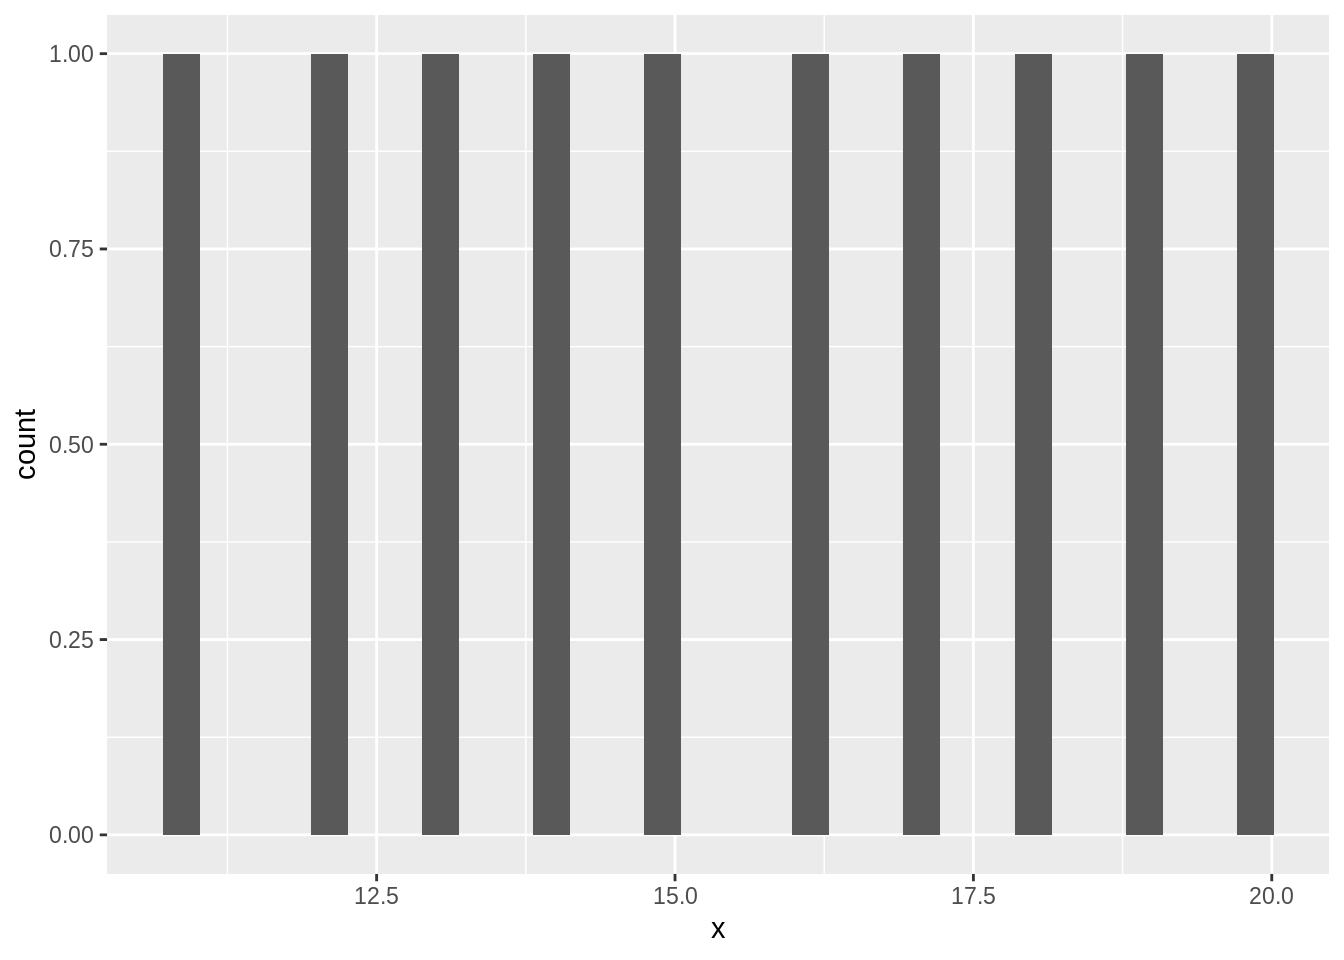
\includegraphics{tidyprog_files/figure-latex/71-no-the-function-is-looking-for-a-variable-named-x-1.pdf}

\begin{Shaded}
\begin{Highlighting}[]
\NormalTok{tidy_histogram <-}\StringTok{ }\ControlFlowTok{function}\NormalTok{(.data, x) \{}
  \CommentTok{# Treat the argument as a variable name}
\NormalTok{  expr <-}\StringTok{ }\KeywordTok{enquo}\NormalTok{(x)}

\NormalTok{  .data }\OperatorTok
\StringTok{    }\CommentTok{# Tell ggplot2 that expr *contains* the name of the variable,}
\StringTok{    }\CommentTok{# instead of expecting a variable named `expr`}
\StringTok{    }\KeywordTok{ggplot}\NormalTok{(}\KeywordTok{aes}\NormalTok{(}\DataTypeTok{x =} \OperatorTok{!!}\NormalTok{expr)) }\OperatorTok{+}
\StringTok{    }\KeywordTok{geom_histogram}\NormalTok{()}
\NormalTok{\}}

\NormalTok{data }\OperatorTok
\StringTok{  }\KeywordTok{tidy_histogram}\NormalTok{(a)}
\end{Highlighting}
\end{Shaded}

\begin{verbatim}
## `stat_bin()` using `bins = 30`. Pick better value with `binwidth`.
\end{verbatim}

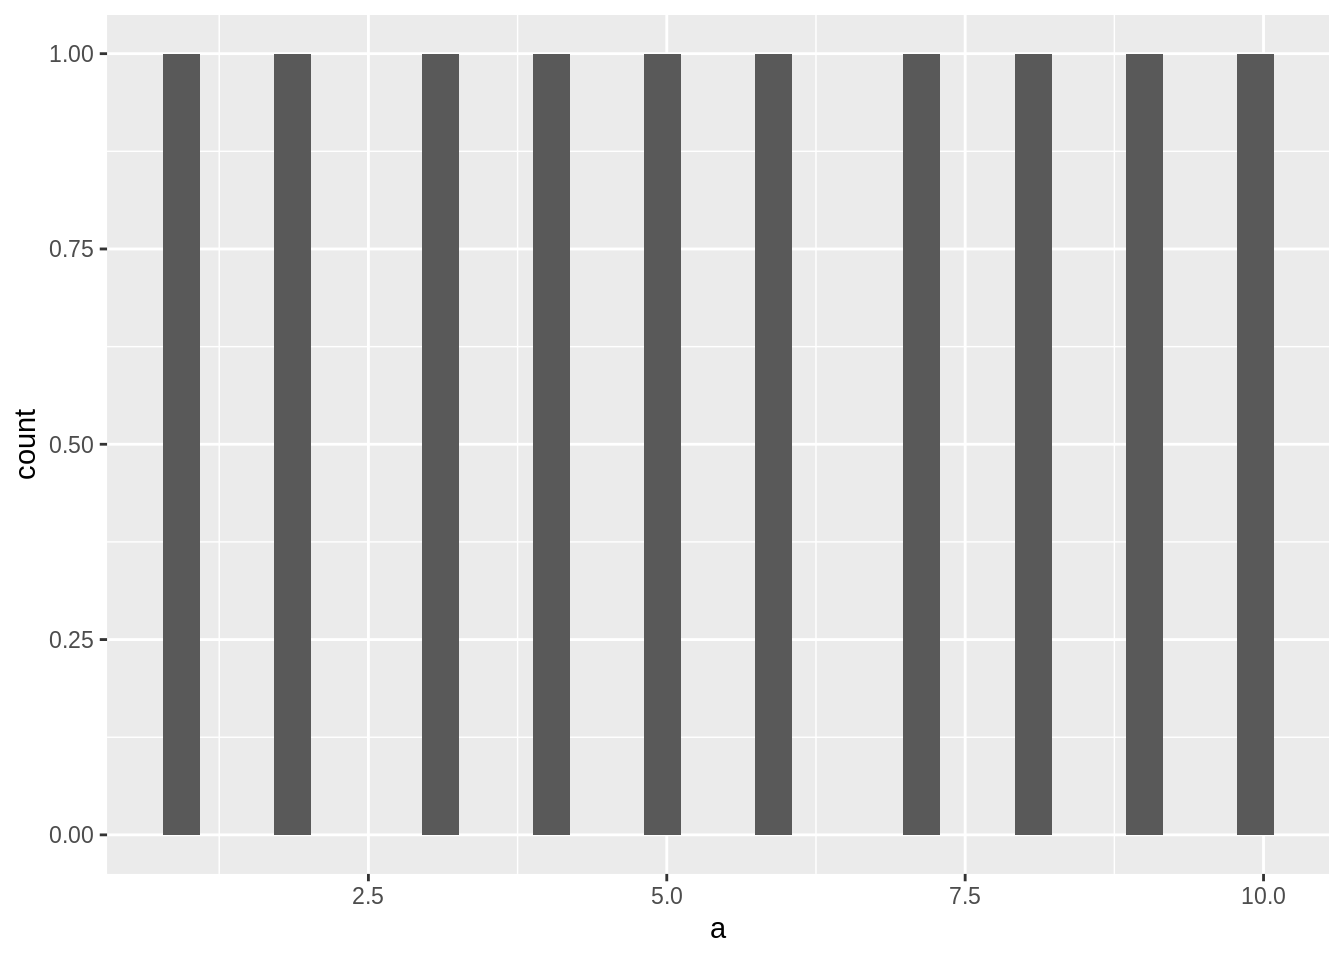
\includegraphics{tidyprog_files/figure-latex/71-solution-quote-unquote-1.pdf}

\begin{Shaded}
\begin{Highlighting}[]
\NormalTok{data }\OperatorTok
\StringTok{  }\KeywordTok{tidy_histogram}\NormalTok{(x)}
\end{Highlighting}
\end{Shaded}

\begin{verbatim}
## `stat_bin()` using `bins = 30`. Pick better value with `binwidth`.
\end{verbatim}

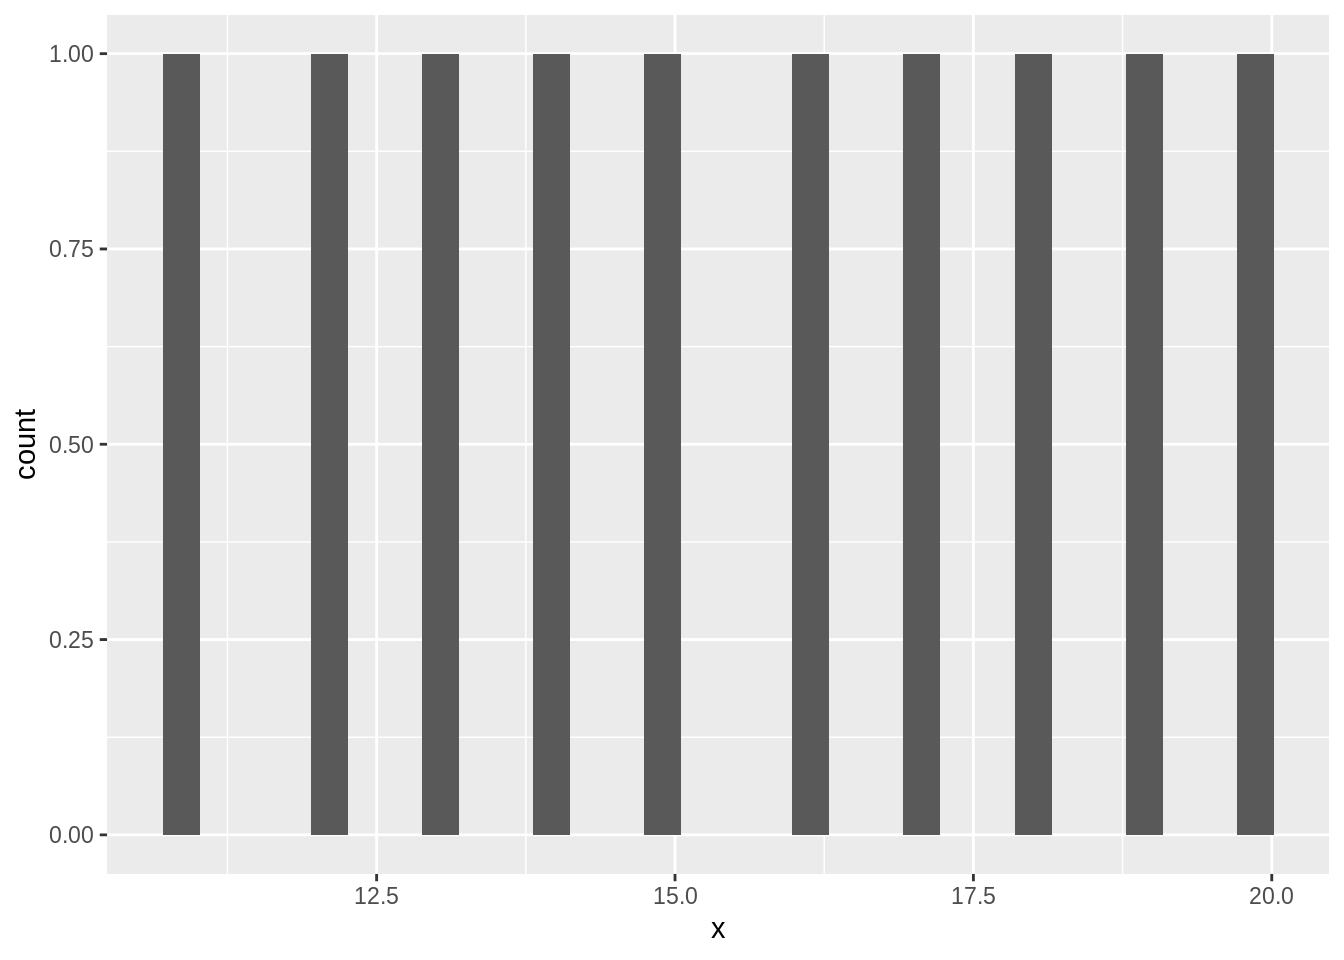
\includegraphics{tidyprog_files/figure-latex/71-solution-quote-unquote-2.pdf}

\begin{Shaded}
\begin{Highlighting}[]
\KeywordTok{try}\NormalTok{(}\KeywordTok{print}\NormalTok{(}
\NormalTok{  data }\OperatorTok
\StringTok{    }\KeywordTok{tidy_histogram}\NormalTok{(y)}
\NormalTok{))}
\end{Highlighting}
\end{Shaded}


\includegraphics{tidyprog_files/figure-latex/71-solution-quote-unquote-3.pdf}

\begin{verbatim}
## Error in FUN(X[[i]], ...) : object 'y' not found
\end{verbatim}

\begin{Shaded}
\begin{Highlighting}[]
\NormalTok{aes}
\end{Highlighting}
\end{Shaded}

\begin{verbatim}
## function (x, y, ...) 
## {
##     exprs <- rlang::enquos(x = x, y = y, ...)
##     is_missing <- vapply(exprs, rlang::quo_is_missing, logical(1))
##     aes <- new_aes(exprs[!is_missing], env = parent.frame())
##     rename_aes(aes)
## }
## <bytecode: 0x7110740>
## <environment: namespace:ggplot2>
\end{verbatim}

\begin{Shaded}
\begin{Highlighting}[]
\NormalTok{mutate_map_dbl <-}\StringTok{ }\ControlFlowTok{function}\NormalTok{(.data, col, expr) \{}
\NormalTok{  quo <-}\StringTok{ }\KeywordTok{enquo}\NormalTok{(col)}

\NormalTok{  .data }\OperatorTok
\StringTok{    }\KeywordTok{mutate}\NormalTok{(}\DataTypeTok{new_column =} \KeywordTok{map_dbl}\NormalTok{(}\OperatorTok{!!}\NormalTok{quo, expr))}
\NormalTok{\}}

\NormalTok{iris_nested <-}
\StringTok{  }\NormalTok{iris }\OperatorTok
\StringTok{  }\KeywordTok{nest}\NormalTok{(}\OperatorTok{-}\NormalTok{Species)}

\NormalTok{iris_nested }\OperatorTok
\StringTok{  }\KeywordTok{mutate_map_dbl}\NormalTok{(data, }\OperatorTok{~}\StringTok{ }\KeywordTok{mean}\NormalTok{(.}\OperatorTok{$}\NormalTok{Petal.Width))}
\end{Highlighting}
\end{Shaded}

\begin{verbatim}
## # A tibble: 3 x 3
##   Species    data              new_column
##   <fct>      <list>                 <dbl>
## 1 setosa     <tibble [50 x 4]>      0.246
## 2 versicolor <tibble [50 x 4]>      1.33 
## 3 virginica  <tibble [50 x 4]>      2.03
\end{verbatim}

\hypertarget{do-yo-need-tidy-evaluation}{%
\section{Do yo need tidy evaluation?}\label{do-yo-need-tidy-evaluation}}

\emph{Click here to show setup code.}

\begin{Shaded}
\begin{Highlighting}[]
\KeywordTok{library}\NormalTok{(tidyverse)}
\end{Highlighting}
\end{Shaded}

\begin{Shaded}
\begin{Highlighting}[]
\NormalTok{summarize_ungroup <-}\StringTok{ }\ControlFlowTok{function}\NormalTok{(.data, ...) \{}
\NormalTok{  .data }\OperatorTok
\StringTok{    }\KeywordTok{summarize}\NormalTok{(...) }\OperatorTok
\StringTok{    }\KeywordTok{ungroup}\NormalTok{()}
\NormalTok{\}}
\end{Highlighting}
\end{Shaded}

\begin{Shaded}
\begin{Highlighting}[]
\NormalTok{mean_airtime_per_day <-}
\StringTok{  }\NormalTok{nycflights13}\OperatorTok{::}\NormalTok{flights }\OperatorTok
\StringTok{  }\KeywordTok{group_by}\NormalTok{(year, month, day) }\OperatorTok
\StringTok{  }\KeywordTok{summarize_ungroup}\NormalTok{(}\KeywordTok{mean}\NormalTok{(air_time, }\DataTypeTok{na.rm =} \OtherTok{TRUE}\NormalTok{))}

\NormalTok{mean_airtime_per_day}
\end{Highlighting}
\end{Shaded}

\begin{verbatim}
## # A tibble: 365 x 4
##    year month   day `mean(air_time, na.rm = TRUE)`
##   <int> <int> <int>                          <dbl>
## 1  2013     1     1                           170.
## 2  2013     1     2                           162.
## 3  2013     1     3                           157.
## # ... with 362 more rows
\end{verbatim}

\begin{Shaded}
\begin{Highlighting}[]
\NormalTok{mean_airtime_per_day }\OperatorTok
\StringTok{  }\KeywordTok{groups}\NormalTok{()}
\end{Highlighting}
\end{Shaded}

\begin{verbatim}
## NULL
\end{verbatim}

\hypertarget{explicit-quote-unquote-of-ellipsis}{%
\section{Explicit quote-unquote of ellipsis}\label{explicit-quote-unquote-of-ellipsis}}

\emph{Click here to show setup code.}

\begin{Shaded}
\begin{Highlighting}[]
\KeywordTok{library}\NormalTok{(tidyverse)}
\KeywordTok{library}\NormalTok{(rlang)}
\end{Highlighting}
\end{Shaded}

\begin{Shaded}
\begin{Highlighting}[]
\NormalTok{summarize_ungroup <-}\StringTok{ }\ControlFlowTok{function}\NormalTok{(.data, ...) \{}
  \CommentTok{# Capture (quote) with enquos()}
\NormalTok{  quos <-}\StringTok{ }\KeywordTok{enquos}\NormalTok{(...)}

  \CommentTok{# Use (unquote-splice) with !!!}
\NormalTok{  .data }\OperatorTok
\StringTok{    }\KeywordTok{summarize}\NormalTok{(}\OperatorTok{!!!}\NormalTok{quos) }\OperatorTok
\StringTok{    }\KeywordTok{ungroup}\NormalTok{()}
\NormalTok{\}}
\end{Highlighting}
\end{Shaded}

\begin{Shaded}
\begin{Highlighting}[]
\NormalTok{mean_airtime_per_day <-}
\StringTok{  }\NormalTok{nycflights13}\OperatorTok{::}\NormalTok{flights }\OperatorTok
\StringTok{  }\KeywordTok{group_by}\NormalTok{(year, month, day) }\OperatorTok
\StringTok{  }\KeywordTok{summarize_ungroup}\NormalTok{(}\KeywordTok{mean}\NormalTok{(air_time, }\DataTypeTok{na.rm =} \OtherTok{TRUE}\NormalTok{))}

\NormalTok{mean_airtime_per_day}
\end{Highlighting}
\end{Shaded}

\begin{verbatim}
## # A tibble: 365 x 4
##    year month   day `mean(air_time, na.rm = TRUE)`
##   <int> <int> <int>                          <dbl>
## 1  2013     1     1                           170.
## 2  2013     1     2                           162.
## 3  2013     1     3                           157.
## # ... with 362 more rows
\end{verbatim}

\begin{Shaded}
\begin{Highlighting}[]
\NormalTok{mean_airtime_per_day }\OperatorTok
\StringTok{  }\KeywordTok{groups}\NormalTok{()}
\end{Highlighting}
\end{Shaded}

\begin{verbatim}
## NULL
\end{verbatim}

\begin{Shaded}
\begin{Highlighting}[]
\NormalTok{aes}
\end{Highlighting}
\end{Shaded}

\begin{verbatim}
## function (x, y, ...) 
## {
##     exprs <- rlang::enquos(x = x, y = y, ...)
##     is_missing <- vapply(exprs, rlang::quo_is_missing, logical(1))
##     aes <- new_aes(exprs[!is_missing], env = parent.frame())
##     rename_aes(aes)
## }
## <bytecode: 0x7110740>
## <environment: namespace:ggplot2>
\end{verbatim}

\hypertarget{names-1}{%
\section{Names}\label{names-1}}

\emph{Click here to show setup code.}

\begin{Shaded}
\begin{Highlighting}[]
\KeywordTok{library}\NormalTok{(tidyverse)}
\KeywordTok{library}\NormalTok{(rlang)}
\end{Highlighting}
\end{Shaded}

\begin{Shaded}
\begin{Highlighting}[]
\NormalTok{gsu <-}\StringTok{ }\ControlFlowTok{function}\NormalTok{(.data, ...) \{}
  \CommentTok{# Capture (quote) with enquos()}
\NormalTok{  quos <-}\StringTok{ }\KeywordTok{enquos}\NormalTok{(...)}

\NormalTok{  is_named <-}\StringTok{ }\NormalTok{(}\KeywordTok{names2}\NormalTok{(quos) }\OperatorTok{!=}\StringTok{ ""}\NormalTok{)}
\NormalTok{  named_quos <-}\StringTok{ }\NormalTok{quos[is_named]}
\NormalTok{  unnamed_quos <-}\StringTok{ }\NormalTok{quos[}\OperatorTok{!}\NormalTok{is_named]}

  \CommentTok{# Use (unquote-splice) with !!!}
\NormalTok{  .data }\OperatorTok
\StringTok{    }\KeywordTok{group_by}\NormalTok{(}\OperatorTok{!!!}\NormalTok{unnamed_quos) }\OperatorTok
\StringTok{    }\KeywordTok{summarize}\NormalTok{(}\OperatorTok{!!!}\NormalTok{named_quos) }\OperatorTok
\StringTok{    }\KeywordTok{ungroup}\NormalTok{()}
\NormalTok{\}}
\end{Highlighting}
\end{Shaded}

\begin{Shaded}
\begin{Highlighting}[]
\NormalTok{mean_airtime_per_day <-}
\StringTok{  }\NormalTok{nycflights13}\OperatorTok{::}\NormalTok{flights }\OperatorTok
\StringTok{  }\KeywordTok{gsu}\NormalTok{(year, month, day, }\DataTypeTok{mean_air_time =} \KeywordTok{mean}\NormalTok{(air_time, }\DataTypeTok{na.rm =} \OtherTok{TRUE}\NormalTok{))}

\NormalTok{mean_airtime_per_day}
\end{Highlighting}
\end{Shaded}

\begin{verbatim}
## # A tibble: 365 x 4
##    year month   day mean_air_time
##   <int> <int> <int>         <dbl>
## 1  2013     1     1          170.
## 2  2013     1     2          162.
## 3  2013     1     3          157.
## # ... with 362 more rows
\end{verbatim}

\hypertarget{section}{%
\section{}\label{section}}

\emph{Click here to show setup code.}

\begin{Shaded}
\begin{Highlighting}[]
\KeywordTok{library}\NormalTok{(rlang)}
\end{Highlighting}
\end{Shaded}

\begin{Shaded}
\begin{Highlighting}[]
\KeywordTok{quos}\NormalTok{(}\DataTypeTok{x =}\NormalTok{ a)}
\end{Highlighting}
\end{Shaded}

\begin{verbatim}
## $x
## <quosure>
## expr: ^a
## env:  0x3336108
\end{verbatim}

\begin{Shaded}
\begin{Highlighting}[]
\NormalTok{a <-}\StringTok{ }\KeywordTok{sym}\NormalTok{(}\StringTok{"b"}\NormalTok{)}
\NormalTok{x_quos <-}\StringTok{ }\KeywordTok{quos}\NormalTok{(}\DataTypeTok{x =} \OperatorTok{!!}\NormalTok{a)}
\NormalTok{x_quos}
\end{Highlighting}
\end{Shaded}

\begin{verbatim}
## $x
## <quosure>
## expr: ^b
## env:  0x3336108
\end{verbatim}

\begin{Shaded}
\begin{Highlighting}[]
\KeywordTok{quos}\NormalTok{(}\DataTypeTok{y =}\NormalTok{ c, }\OperatorTok{!!!}\NormalTok{x_quos)}
\end{Highlighting}
\end{Shaded}

\begin{verbatim}
## $y
## <quosure>
## expr: ^c
## env:  0x3336108
## 
## $x
## <quosure>
## expr: ^b
## env:  0x3336108
\end{verbatim}

\hypertarget{section-1}{%
\section{}\label{section-1}}

\emph{Click here to show setup code.}

\begin{Shaded}
\begin{Highlighting}[]
\KeywordTok{library}\NormalTok{(tidyverse)}
\KeywordTok{library}\NormalTok{(rlang)}
\end{Highlighting}
\end{Shaded}

\begin{Shaded}
\begin{Highlighting}[]
\NormalTok{mutate_map_dbl <-}\StringTok{ }\ControlFlowTok{function}\NormalTok{(.data, col, ...) \{}
\NormalTok{  quos <-}\StringTok{ }\KeywordTok{build_quos}\NormalTok{(}\OperatorTok{!!}\KeywordTok{enquo}\NormalTok{(col), ...)}
\NormalTok{  .data }\OperatorTok
\StringTok{    }\KeywordTok{mutate}\NormalTok{(}\OperatorTok{!!!}\NormalTok{quos)}
\NormalTok{\}}

\NormalTok{build_quos <-}\StringTok{ }\ControlFlowTok{function}\NormalTok{(col, ...) \{}
\NormalTok{  args <-}\StringTok{ }\KeywordTok{list}\NormalTok{(...)}
  \KeywordTok{stopifnot}\NormalTok{(}\KeywordTok{length}\NormalTok{(args) }\OperatorTok{==}\StringTok{ }\DecValTok{1}\NormalTok{)}

\NormalTok{  expr <-}\StringTok{ }\NormalTok{args[[}\DecValTok{1}\NormalTok{]]}

\NormalTok{  map_quo <-}\StringTok{ }\KeywordTok{build_map_quo}\NormalTok{(}\OperatorTok{!!}\KeywordTok{enquo}\NormalTok{(col), expr)}

  \KeywordTok{set_names}\NormalTok{(}\KeywordTok{list}\NormalTok{(map_quo), }\KeywordTok{names}\NormalTok{(args))}
\NormalTok{\}}

\NormalTok{build_map_quo <-}\StringTok{ }\ControlFlowTok{function}\NormalTok{(col, expr) \{}
\NormalTok{  quo <-}\StringTok{ }\KeywordTok{enquo}\NormalTok{(col)}
  \KeywordTok{quo}\NormalTok{(}\KeywordTok{map_dbl}\NormalTok{(}\OperatorTok{!!}\NormalTok{quo, expr))}
\NormalTok{\}}
\end{Highlighting}
\end{Shaded}

\begin{Shaded}
\begin{Highlighting}[]
\KeywordTok{build_quos}\NormalTok{(data, }\DataTypeTok{mean_petal_width =} \OperatorTok{~}\StringTok{ }\KeywordTok{mean}\NormalTok{(.}\OperatorTok{$}\NormalTok{Petal.Width))}
\end{Highlighting}
\end{Shaded}

\begin{verbatim}
## $mean_petal_width
## <quosure>
## expr: ^map_dbl(^data, expr)
## env:  0x9a0c148
\end{verbatim}

\begin{Shaded}
\begin{Highlighting}[]
\KeywordTok{build_map_quo}\NormalTok{(mean_petal_width, }\OperatorTok{~}\StringTok{ }\KeywordTok{mean}\NormalTok{(.}\OperatorTok{$}\NormalTok{Petal.Width))}
\end{Highlighting}
\end{Shaded}

\begin{verbatim}
## <quosure>
## expr: ^map_dbl(^mean_petal_width, expr)
## env:  0xb632bd0
\end{verbatim}

\begin{Shaded}
\begin{Highlighting}[]
\NormalTok{iris }\OperatorTok
\StringTok{  }\KeywordTok{nest}\NormalTok{(}\OperatorTok{-}\NormalTok{Species) }\OperatorTok
\StringTok{  }\KeywordTok{mutate_map_dbl}\NormalTok{(data, }\DataTypeTok{mean_petal_width =} \OperatorTok{~}\StringTok{ }\KeywordTok{mean}\NormalTok{(.}\OperatorTok{$}\NormalTok{Petal.Width))}
\end{Highlighting}
\end{Shaded}

\begin{verbatim}
## # A tibble: 3 x 3
##   Species    data              mean_petal_width
##   <fct>      <list>                       <dbl>
## 1 setosa     <tibble [50 x 4]>            0.246
## 2 versicolor <tibble [50 x 4]>            1.33 
## 3 virginica  <tibble [50 x 4]>            2.03
\end{verbatim}

\hypertarget{section-2}{%
\section{}\label{section-2}}

\emph{Click here to show setup code.}

\begin{Shaded}
\begin{Highlighting}[]
\KeywordTok{library}\NormalTok{(tidyverse)}
\KeywordTok{library}\NormalTok{(rlang)}

\NormalTok{mutate_map_dbl <-}\StringTok{ }\ControlFlowTok{function}\NormalTok{(.data, col, ...) \{}
\NormalTok{  quos <-}\StringTok{ }\KeywordTok{build_quos}\NormalTok{(}\OperatorTok{!!}\KeywordTok{enquo}\NormalTok{(col), ...)}
\NormalTok{  .data }\OperatorTok
\StringTok{    }\KeywordTok{mutate}\NormalTok{(}\OperatorTok{!!!}\NormalTok{quos)}
\NormalTok{\}}
\end{Highlighting}
\end{Shaded}

\begin{Shaded}
\begin{Highlighting}[]
\NormalTok{build_quos <-}\StringTok{ }\ControlFlowTok{function}\NormalTok{(col, ...) \{}
\NormalTok{  args <-}\StringTok{ }\KeywordTok{enquos}\NormalTok{(...)}
  \KeywordTok{stopifnot}\NormalTok{(}\KeywordTok{length}\NormalTok{(args) }\OperatorTok{==}\StringTok{ }\DecValTok{1}\NormalTok{)}

\NormalTok{  expr <-}\StringTok{ }\NormalTok{args[[}\DecValTok{1}\NormalTok{]]}

\NormalTok{  map_quo <-}\StringTok{ }\KeywordTok{build_map_quo}\NormalTok{(}\OperatorTok{!!}\KeywordTok{enquo}\NormalTok{(col), }\OperatorTok{!!}\NormalTok{expr)}

  \KeywordTok{set_names}\NormalTok{(}\KeywordTok{list}\NormalTok{(map_quo), }\KeywordTok{names}\NormalTok{(args))}
\NormalTok{\}}

\NormalTok{build_map_quo <-}\StringTok{ }\ControlFlowTok{function}\NormalTok{(col, expr) \{}
\NormalTok{  quo <-}\StringTok{ }\KeywordTok{enquo}\NormalTok{(col)}
\NormalTok{  mapper <-}\StringTok{ }\KeywordTok{as_mapper_quosure}\NormalTok{(}\OperatorTok{!!}\KeywordTok{enquo}\NormalTok{(expr))}
  \KeywordTok{quo}\NormalTok{(}\KeywordTok{map_dbl}\NormalTok{(}\OperatorTok{!!}\NormalTok{quo, }\OperatorTok{!!}\NormalTok{mapper))}
\NormalTok{\}}

\NormalTok{as_mapper_quosure <-}\StringTok{ }\ControlFlowTok{function}\NormalTok{(expr) \{}
\NormalTok{  quo <-}\StringTok{ }\KeywordTok{enquo}\NormalTok{(expr)}

\NormalTok{  rlang}\OperatorTok{::}\KeywordTok{new_function}\NormalTok{(}\KeywordTok{alist}\NormalTok{(}\DataTypeTok{... =}\NormalTok{ , }\DataTypeTok{. =}\NormalTok{ ..}\DecValTok{1}\NormalTok{, }\DataTypeTok{.x =}\NormalTok{ ..}\DecValTok{1}\NormalTok{, }\DataTypeTok{.y =}\NormalTok{ ..}\DecValTok{2}\NormalTok{), }\KeywordTok{quo_get_expr}\NormalTok{(quo))}
\NormalTok{\}}
\end{Highlighting}
\end{Shaded}

\begin{Shaded}
\begin{Highlighting}[]
\KeywordTok{as_mapper}\NormalTok{(}\OperatorTok{~}\StringTok{ }\KeywordTok{mean}\NormalTok{(.}\OperatorTok{$}\NormalTok{Petal.Width))}
\end{Highlighting}
\end{Shaded}

\begin{verbatim}
## <lambda>
## function (..., .x = ..1, .y = ..2, . = ..1) 
## mean(.$Petal.Width)
## <environment: 0x3336108>
## attr(,"class")
## [1] "rlang_lambda_function"
\end{verbatim}

\begin{Shaded}
\begin{Highlighting}[]
\KeywordTok{as_mapper_quosure}\NormalTok{(}\KeywordTok{mean}\NormalTok{(.}\OperatorTok{$}\NormalTok{Petal.Width))}
\end{Highlighting}
\end{Shaded}

\begin{verbatim}
## function (..., . = ..1, .x = ..1, .y = ..2) 
## mean(.$Petal.Width)
## <environment: 0x97ba9e0>
\end{verbatim}

\begin{Shaded}
\begin{Highlighting}[]
\KeywordTok{build_map_quo}\NormalTok{(mean_petal_width, }\KeywordTok{mean}\NormalTok{(.}\OperatorTok{$}\NormalTok{Petal.Width))}
\end{Highlighting}
\end{Shaded}

\begin{verbatim}
## <quosure>
## expr: ^map_dbl(^mean_petal_width, <function(..., . = ..1, .x = ..1,
##           .y = ..2) mean(.$Petal.Width)>)
## env:  0xc4f8ca0
\end{verbatim}

\begin{Shaded}
\begin{Highlighting}[]
\NormalTok{iris }\OperatorTok
\StringTok{  }\KeywordTok{nest}\NormalTok{(}\OperatorTok{-}\NormalTok{Species) }\OperatorTok
\StringTok{  }\KeywordTok{mutate_map_dbl}\NormalTok{(data, }\DataTypeTok{mean_petal_width =} \KeywordTok{mean}\NormalTok{(.}\OperatorTok{$}\NormalTok{Petal.Width))}
\end{Highlighting}
\end{Shaded}

\begin{verbatim}
## # A tibble: 3 x 3
##   Species    data              mean_petal_width
##   <fct>      <list>                       <dbl>
## 1 setosa     <tibble [50 x 4]>            0.246
## 2 versicolor <tibble [50 x 4]>            1.33 
## 3 virginica  <tibble [50 x 4]>            2.03
\end{verbatim}

\hypertarget{best-practices}{%
\chapter{Best practices}\label{best-practices}}

R code is often organized in packages that can be installed from centralized repositories such as CRAN or GitHub.
If you are new to writing R packages, this course cannot give a complete introduction into packages.
It is still useful to embrace some very few concepts of R packages to gain access to a vast toolbox and also organize your code in a standardized way familiar to other users.
With the first steps in place, the road to your first R package may become less steep.

\begin{itemize}
\tightlist
\item
  Create a \texttt{DESCRIPTION} file to declare dependencies and allow easy reloading of the functions you define
\item
  Store your functions in \texttt{.R} files in the \texttt{R/} directory in your project

  \begin{itemize}
  \tightlist
  \item
    Scripts that you execute live in \texttt{script/} or a similar directory
  \end{itemize}
\item
  Use \href{https://github.com/klutometis/roxygen}{roxygen2} to document your functions close to the source
\item
  Write tests for your functions, e.g.~with \href{https://testthat.r-lib.org/}{testthat}
\end{itemize}

See \href{http://r-pkgs.had.co.nz/}{R packages} for a more comprehensive treatment.

\hypertarget{description}{%
\section{DESCRIPTION}\label{description}}

Create and open a new RStudio project.
Then, create a \texttt{DESCRIPTION} file with \texttt{usethis::use\_description()}:

\begin{Shaded}
\begin{Highlighting}[]
\CommentTok{# install.packages("usethis")}
\NormalTok{usethis}\OperatorTok{::}\KeywordTok{use_description}\NormalTok{()}
\end{Highlighting}
\end{Shaded}

Double-check success:

\begin{Shaded}
\begin{Highlighting}[]
\CommentTok{# install.packages("devtools")}
\NormalTok{devtools}\OperatorTok{::}\KeywordTok{load_all}\NormalTok{()}
\end{Highlighting}
\end{Shaded}

Declare that your project requires the tidyverse and the here package:

\begin{Shaded}
\begin{Highlighting}[]
\NormalTok{usethis}\OperatorTok{::}\KeywordTok{use_package}\NormalTok{(}\StringTok{"here"}\NormalTok{)}
\CommentTok{# Currently doesn't work, add manually}
\CommentTok{# https://github.com/r-lib/usethis/issues/760}
\CommentTok{# usethis::use_package("tidyverse")}
\end{Highlighting}
\end{Shaded}

\hypertarget{r}{%
\section{R}\label{r}}

With a \texttt{DESCRIPTION} file defined, create a new \texttt{.R} file and save it in the \texttt{R/} directory.
(Create this directory if it does not exist.)
Create a function in this file, save the file:

\begin{Shaded}
\begin{Highlighting}[]
\NormalTok{hi <-}\StringTok{ }\ControlFlowTok{function}\NormalTok{(}\DataTypeTok{text =} \StringTok{"Hello, world!"}\NormalTok{) \{}
  \KeywordTok{print}\NormalTok{(text)}
  \KeywordTok{invisible}\NormalTok{(text)}
\NormalTok{\}}
\end{Highlighting}
\end{Shaded}

Do not source the file.

Restart R (with Ctrl + Shift + F10 in RStudio).

Run \texttt{devtools::load\_all()} again, you can use the shortcut Ctrl + Shift + L or Cmd + Shift + L in RStudio.

Check that you can run \texttt{hi()} in the console:

\begin{Shaded}
\begin{Highlighting}[]
\KeywordTok{hi}\NormalTok{()}
\end{Highlighting}
\end{Shaded}

\begin{verbatim}
## [1] "Hello, world!"
\end{verbatim}

\begin{Shaded}
\begin{Highlighting}[]
\KeywordTok{hi}\NormalTok{(}\StringTok{"Wow!"}\NormalTok{)}
\end{Highlighting}
\end{Shaded}

\begin{verbatim}
## [1] "Wow!"
\end{verbatim}

Edit the function:

\begin{Shaded}
\begin{Highlighting}[]
\NormalTok{hi <-}\StringTok{ }\ControlFlowTok{function}\NormalTok{(}\DataTypeTok{text =} \StringTok{"Wow!"}\NormalTok{) \{}
  \KeywordTok{print}\NormalTok{(text)}
  \KeywordTok{invisible}\NormalTok{(text)}
\NormalTok{\}}
\end{Highlighting}
\end{Shaded}

Save the file, but do not source it.

Run \texttt{devtools::load\_all()} again, you can use the shortcut Ctrl + Shift + L or Cmd + Shift + L in RStudio.

Check that the new implementation of \texttt{hi()} is active:

\begin{Shaded}
\begin{Highlighting}[]
\KeywordTok{hi}\NormalTok{()}
\end{Highlighting}
\end{Shaded}

\begin{verbatim}
## [1] "Wow!"
\end{verbatim}

All functions that are required for your project are stored in this directory.
Do not store executable scripts, use a \texttt{script/} directory.

\hypertarget{roxygen2}{%
\section{roxygen2}\label{roxygen2}}

The following intuitive annotation syntax is a standard way to create documentation for your functions:

\begin{Shaded}
\begin{Highlighting}[]
\CommentTok{#' Print a welcome message}
\CommentTok{#' }
\CommentTok{#' This function prints "Wow!", or a custom text, on the console.}
\CommentTok{#'}
\CommentTok{#' @param text The text to print, "Wow!" by default.}
\CommentTok{#' }
\CommentTok{#' @return The `text` argument, invisibly.}
\CommentTok{#' }
\CommentTok{#' @examples}
\CommentTok{#' hi()}
\CommentTok{#' hi("Hello!")}
\NormalTok{hi <-}\StringTok{ }\ControlFlowTok{function}\NormalTok{(}\DataTypeTok{text =} \StringTok{"Wow!"}\NormalTok{) \{}
  \KeywordTok{print}\NormalTok{(text)}
  \KeywordTok{invisible}\NormalTok{(text)}
\NormalTok{\}}
\end{Highlighting}
\end{Shaded}

This annotation can be rendered to a nicely looking HTML page with the roxygen2 and pkgdown packages.
All you need to do is provide (and maintain) it.

\hypertarget{testthat}{%
\section{testthat}\label{testthat}}

Automated tests make sure that the functions you write today continue working tomorrow.
Create your first test with \texttt{usethis::use\_test()}:

\begin{Shaded}
\begin{Highlighting}[]
\CommentTok{# install.packages("testthat")}
\NormalTok{usethis}\OperatorTok{::}\KeywordTok{use_test}\NormalTok{(}\StringTok{"hi"}\NormalTok{)}
\end{Highlighting}
\end{Shaded}

The file \texttt{tests/testthat/test-hi.R} is created, with the following contents:

\begin{Shaded}
\begin{Highlighting}[]
\KeywordTok{test_that}\NormalTok{(}\StringTok{"multiplication works"}\NormalTok{, \{}
  \KeywordTok{expect_equal}\NormalTok{(}\DecValTok{2} \OperatorTok{*}\StringTok{ }\DecValTok{2}\NormalTok{, }\DecValTok{4}\NormalTok{)}
\NormalTok{\})}
\end{Highlighting}
\end{Shaded}

Replace this predefined text with a test that makes more sense for us:

\begin{Shaded}
\begin{Highlighting}[]
\KeywordTok{test_that}\NormalTok{(}\StringTok{"hi() works"}\NormalTok{, \{}
  \KeywordTok{expect_output}\NormalTok{(}\KeywordTok{hi}\NormalTok{(), }\StringTok{"Wow"}\NormalTok{)}
  \KeywordTok{expect_output}\NormalTok{(}\KeywordTok{hi}\NormalTok{(}\StringTok{"Hello"}\NormalTok{), }\StringTok{"Hello"}\NormalTok{)}
\NormalTok{\})}
\end{Highlighting}
\end{Shaded}

Run the new test with \texttt{devtools::test()}, you can use the shortcut Ctrl + Shift + T or Cmd + Shift + T in RStudio.

Check that the test actually detects failures by modifying the implementation of \texttt{hi()} and rerunning the test:

\begin{Shaded}
\begin{Highlighting}[]
\NormalTok{hi <-}\StringTok{ }\ControlFlowTok{function}\NormalTok{(}\DataTypeTok{text =} \StringTok{"Oops!"}\NormalTok{) \{}
  \KeywordTok{print}\NormalTok{(text)}
  \KeywordTok{invisible}\NormalTok{(text)}
\NormalTok{\}}
\end{Highlighting}
\end{Shaded}

Run the new test with \texttt{devtools::test()}, you can use the shortcut Ctrl + Shift + T or Cmd + Shift + T in RStudio.
One test should be failing now.

\hypertarget{section-3}{%
\chapter{}\label{section-3}}

\begin{itemize}
\item
  R for data science: \url{https://r4ds.had.co.nz/}
\item
  Row oriented workflows: \url{https://github.com/jennybc/row-oriented-workflows\#readme}
\item
  Advanced R: \url{http://adv-r.had.co.nz/}
\item
  Tidy evaluation: \url{https://tidyeval.tidyverse.org/}
\item
  R packages: \url{http://r-pkgs.had.co.nz/}
\item
  roxygen2: Vignettes in \url{https://cran.r-project.org/package=roxygen2}, especially:

  \begin{itemize}
  \item
    \href{https://cran.r-project.org/web/packages/roxygen2/vignettes/roxygen2.html}{Introduction to roxygen2}
  \item
    \href{https://cran.r-project.org/web/packages/roxygen2/vignettes/rd.html}{Generating Rd files} for an overview of available tags
  \item
    \href{https://cran.r-project.org/web/packages/roxygen2/vignettes/markdown.html}{Write R documentation in Markdown}
  \end{itemize}
\item
  How R searches and finds stuff: \url{http://blog.obeautifulcode.com/R/How-R-Searches-And-Finds-Stuff/}
\item
  What they forgot to teach you: \url{https://whattheyforgot.org/}
\item
  Parallel processing with a purrr-like interface: \url{https://davisvaughan.github.io/furrr/}
\item
  Tidyverse principles: \url{https://principles.tidyverse.org/}
\end{itemize}


\end{document}
